\documentclass[11pt]{article}
\usepackage[left=20mm, right=20mm, top=20mm, bottom=20mm]{geometry} %this sets the page margins 
\usepackage{amsmath}
\usepackage{graphicx}
\usepackage{wrapfig}
\usepackage{subcaption}
\usepackage[justification=centering]{caption}
\usepackage{setspace}
\doublespacing
\setlength{\parindent}{1cm}
\usepackage[colorinlistoftodos]{todonotes}
\usepackage{color}
\usepackage{framed}
\usepackage{comment}

\usepackage{courier}
\usepackage{float}
\floatstyle{boxed}
\newfloat{code}{ht}{lop}
\floatname{code}{Extract}

%\usepackage[latin1]{inputenc}
\usepackage[T1]{fontenc}
\usepackage{tikz}
\usetikzlibrary{shapes,arrows}

\usepackage{helvet}
\renewcommand{\familydefault}{\sfdefault}

\usepackage[hyphens]{url}
\usepackage{listings,xcolor}
\definecolor{dkgreen}{rgb}{0,.6,0}
\definecolor{dkblue}{rgb}{0,0,.6}
\definecolor{dkyellow}{cmyk}{0,0,.8,.3}
\definecolor{gray}{rgb}{0.4,0.4,0.4}
\definecolor{darkblue}{rgb}{0.0,0.0,0.6}
\definecolor{cyan}{rgb}{0.0,0.6,0.6}
\definecolor{mauve}{rgb}{0.58,0,0.82}

\lstnewenvironment{php}
{\lstset{language=php,
  aboveskip=3mm,
  belowskip=3mm,
  showstringspaces=false,
  columns=flexible,
  basicstyle={\footnotesize\ttfamily},
  numbers=none,
  numberstyle=\tiny\color{gray},
  keywordstyle=\color{blue},
  commentstyle=\color{dkgreen},
  stringstyle=\color{mauve},
  breakatwhitespace=true,
  breaklines=true,
  tabsize=3,
  lineskip={-2pt}
  }
  }{}
\lstnewenvironment{html}
{\lstset{language=html,
  aboveskip=3mm,
  belowskip=3mm,
  showstringspaces=false,
  columns=flexible,
  basicstyle={\footnotesize\ttfamily},
  numbers=none,
  numberstyle=\tiny\color{gray},
  keywordstyle=\color{blue},
  commentstyle=\color{dkgreen},
  stringstyle=\color{mauve},
  breakatwhitespace=true,
  breaklines=true,
  tabsize=3,
  lineskip={-2pt}
  }
  }{}
\lstdefinelanguage{CSS}{
    sensitive=true,
    alsodigit={-},
    keywords={transform, transition-property, transition-duration, transition-timing-functio},              
    morecomment=[l]{//},
    morecomment=[s]{/*}{*/},
    morestring=[b]',
    morestring=[b]"
}
\lstnewenvironment{css}
{\lstset{language=css,
  aboveskip=3mm,
  belowskip=3mm,
  showstringspaces=false,
  columns=flexible,
  basicstyle={\footnotesize\ttfamily},
  numbers=none,
  numberstyle=\tiny\color{gray},
  keywordstyle=\color{blue},
  commentstyle=\color{dkgreen},
  stringstyle=\color{mauve},
  breakatwhitespace=true,
  breaklines=true,
  tabsize=3,
  lineskip={-2pt}
  }
  }{}


\author{Michael Fedosiuk, Henry Fletcher, Emma Saragossi & Jeffrey Yu}

\title{3yp report Cardiac Track}
\newcommand{\HRule}{\rule{\linewidth}{0.5mm}}

%%%%%%%%%%%%%%%%%%%%%%%%%%%%%%%%%%%%%%%%%%%%%%%%%%%%%%%%%%%%%%%%%%%%%%%%%%%%%%%%%%%%%%%%%%%%%%%%%%%%%%%%%%
\begin{document}


\begin{titlepage}
\begin{center}

% Upper part of the page. The '~' is needed because \\
% only works if a paragraph has started.

\includegraphics[width=0.27\textwidth]{titleimg.png}~\\[1cm]

\textsc{\Large 3rd year project report}\\[0.5cm]

% Title
\HRule \\[0.4cm]
{ \huge \bfseries Cardiac Track Application \\[0.4cm] }

\HRule \\[1.5cm]

% Author and supervisor
\begin{minipage}{0.8\textwidth}
\begin{flushleft} \large
\emph{Authors:}\\
Michael \textsc{Fedosiuk}, Henry \textsc{Fletcher}, Emma \textsc{Saragossi} \& Jeffery \textsc{Yu}
\\
%\emph{Executive Summary:}\\
%This is cardiac track the app we made for our 3yp project
\end{flushleft}
\end{minipage}

\vfill

% Bottom of the page
{\large \today}

\end{center}
\end{titlepage}

\tableofcontents

\section{Design brief and specification - \textit{Emma Saragossi}}
\subsection{Overview}

Our aim is to research, design and build an intelligent software application that will aid clinicians with the pharmacological treatment of primary hypertension\footnote{Note: patients will have already been diagnosed with the condition by a medical professional.}. The application will comprise of two separate web-based applications, one for the doctor and one for the patient, which can both read-from and write-to a shared database. Patients will be able to upload their blood pressure remotely (i.e. not within a clinical setting) to the database on a daily basis. The doctor application will read in the patients' blood pressure data and display it on a chart for the doctor to view. The doctor application will also provide a link to launch a Tallis web decision tool that will advise the doctor on the best course of treatment, based on the patient's medical history, background, and charted blood pressure history.

\subsection{Patient Application}
\begin{itemize}
\item The application must run in a desktop, tablet or mobile web browser.
\item The application must be hosted on a suitable server.
\item The application must have a secure login system, to identify the patient using the application and to prevent others from accessing sensitive patient data.
\item The application must be able to read-from and write-to the shared database.
\item The application must provide a submission form, allowing patient to enter their systolic and diastolic blood pressure values. This data must be uploaded to the database, along with time and date of upload. Note: this may be extended to include other metrics which may be of value (e.g. heart rate, weight etc.).
\item The application must have a charting tool which plots blood pressure values against date, to allow the user to track their progress.
\item The application must provide the contact details for patient's doctor.
\item The application must indicate when the patient is due for a scheduled follow up appointment with their doctor.
\item The application must advise the patient if they should contact their doctor (for example if their blood pressure has not reached the target level, or has risen unexpectedly). An alert should be sent to the doctor if this is the case so that the responsibility is not solely on the patient to make contact.
\end{itemize}

\subsection{Doctor Application}
\begin{itemize}
\item The application must run in a desktop or tablet web browser.
\item The application must be hosted on a suitable server.
\item The application must have a secure login system, which identifies the doctor and allows them access to view only their own patients' profiles.
\item The application must be able to read-from and write-to the shared database.
\item The application must allow the doctor to create a new patient profile.
	\begin{itemize}
    \item The doctor must be able to enter relevant patient data\footnote{The information required to determine the appropriate course of treatment for a patient is defined in NICE Clinical Guideline 127 \cite{CG127}.} (e.g. age, gender, medical history etc.)
    \item The patient's target blood pressure must be determined based on the patient data provided
    \item All patient data must be submitted to the database
    \item Each patient must be assigned a unique Patient ID.
    \item The doctor must be able to assign the patient unique login details for access to the patient application
    \item The patient must meet the scope of the application\footnote{As outlined in NICE Clinical Guideline 127\cite{CG127}.}. The patient profile creation process must terminate if the patient is unsuitable.
	\end{itemize}
\item The application must allow the doctor to view the progress of all their patients
	\begin{itemize}
    \item The doctor must be able to search for the profile of a specific patient using their unique Patient ID
    \item The application must have a charting tool which plots the patient's blood pressure against date, to allow the doctor to monitor their progress
    \item The application must summarize the pharmacological treatment currently being offered to the patient
    \item The application must alert the doctor if the patient has not met their target blood pressure within the expected time range, or if the patient's blood pressure has suddenly risen above the target value.
    \end{itemize}
\item The application must provide a link to launch the Tallis treatment decision tool (see below)
\end{itemize}

\subsection{Tallis Application}
\begin{itemize}
\item The application must run in a desktop or tablet web brower.
\item The application must be hosted on a suitable server.
\item The application must be able to read-from and write-to the database
\item The application must reccommend the best initial course of treatment for the patient based on the patient data submitted during the patient profile creation process.
\item The application must recommend an appropriate drug dosage.
\item The application must schedule an appropriate review date, by which time the target blood pressure should be met.
\item The application must allow the doctor to review the patient
	\begin{itemize}
    \item The application must allow the doctor to perform a titration assessment of the patient and upload the values to the database.
    \item The application must recommend a secondary drug treatment or allow the doctor to update the dosage of previously prescribed drug if the patient's target blood pressure has not been met.
    \item The review-recommendation process must cycle until the patient's target blood pressure has been met.
    \end{itemize}
\item All medical recommendations must be made in accordance with the relevant medical guideline \cite{CG127}.
\end{itemize}

\subsection{Database}
\begin{itemize}
\item The database must be hosted on a server
\item The database must be able to send and receive data from both the patient and doctor application (including the Tallis decision tool)
\item The database must be structured to store:
	\begin{itemize}
	\item A doctor access log
    \item Doctor login information
    \item Patient information (including their doctor, medical history, target blood pressure, login details, drug type etc)
    \item Patient blood pressure data and the time and date of upload
	\end{itemize}
\item The database must meet the encryption standard expected of medical software set by the NHS \cite{encryption}
\item The database must allow multiple users to read-from and write-to the database at the same time. 
\end{itemize}

\begin{figure}[ht]
\begin{center}
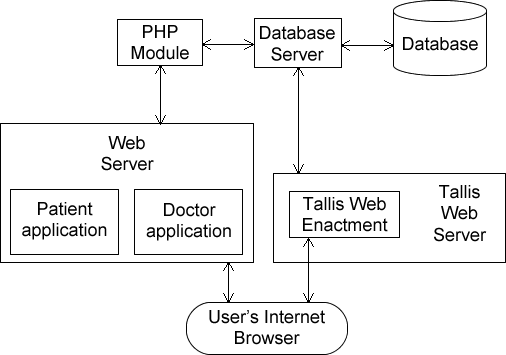
\includegraphics[scale=0.5]{network}
\caption{Overall architecture of software application}
\label{fig:network}
\end{center}
\end{figure}

%%%%%%%%%%%%%%%%%%%%%%%%%%%%%%%%%%%%%%%%%%%%%%%%%%%%%%%%%%%%%%%%%%%%%%%%%%%%%%%%%%%%%%%%%%%%%%%%%%%%%%%%%%%

\section{Clinical need - \textit{Emma Saragossi}}
Hypertension is one of the most common conditions treated by primary care in the United Kingdom, affecting more than a quarter of all adults and more than half of those aged 65 years and over \cite{surveyEngland2009}. As it is such a common condition, it places a heavy strain on NHS resources. Our aim is to reduce the amount of contact time between doctors and patients, freeing doctors to better spend their time elsewhere. Remote monitoring of patients' blood pressure ensures that the doctor only need meet the patient for a consultation or check up when necessary. One of the key functions of our application is that it will alert the doctor if a patient's blood pressure is not at the target level, meaning appointments are only scheduled when there is clinical need.

The treatment of hypertension has relied on blood pressure measurements made within a clinical setting for over 100 years \cite{SICC}, but this method of recording blood pressure has its limitations. A single blood pressure reading made at a primary care facility may not represent a patient's true blood pressure; blood pressure changes continuously over time, and is sensitive to both random and systematic errors (e.g. white coat effect). An alternative is to allow the patient to record their own blood pressure at home. A major advantage of out-of-office blood pressure monitoring is that it provides a large number of blood pressure measurements made away from a medical setting, better reflecting the patient's blood pressure during usual daytime activities \cite{ESH}. As a result of this more reliable measure of blood pressure, more suitable treatment decisions can be made.

In addition to providing more accurate and reliable data, home monitoring of hypertension empowers the patient, influencing their attitude and behaviour. The NICE clinical guideline for the management of primary hypertension in adults recognises that engaging patients in their own blood pressure monitoring process could lead to improved blood pressure control \cite{CG127}. Moreover, a meta-analysis by Bray et al., 2010 \cite{metaSelfMonitoring} showed that patients who self-monitor their own blood pressure have an increased chance of achieving their target blood pressure.

The online treatment aid implements the most up to date NICE guidelines for the management of hypertension. This can be regularly updated to implement best practice and ensure the doctor is offering consistent, high quality, safe and accountable care.

%%%%%%%%%%%%%%%%%%%%%%%%%%%%%%%%%%%%%%%%%%%%%%%%%%%%%%%%%%%%%%%%%%%%%%%%%%%%%%%%%%%%%%%%%%%%%%%%%%%%%%%%%

\section{Application User Interface - \textit{Michael Fedosiuk}}
The user interface (UI) for the Cardiac Track application is in two parts. There is a patient app, currently optimised for smartphones, where BP measurements are inputted and the patient is alerted to make an appointment with their GP when they breach their BP limit. The app also provides the patient with their GP contact details and a graphical representation of their historical BP data.
\\ \indent
The second part is a doctor app, currently optimised for desktops and tablets, which allows the doctor to check up on the details of any of their patients. It alerts them to which have breached their targets, and provides suggestions on how to best medicate their hypertension on an individual basis. 

\subsection{Why a Web based application was chosen and what languages were used}
The UI has been written in HTML5, CSS3, Javascript and JQuery. All these languages are standard in web development. An initial design decision for the project was whether to code the UI in either a web-based format using these languages or to instead create a native application. The two most common types of native application are those programmed in iOS or Android, these are download from an app store and then run on the devices own operating system. The benefit from having a native application is that they can be more complex and an Internet connection is not required for the application to run. The major limitation to native applications is that the programming syntax for iOS and Android are different, meaning that the same application must be coded twice. Therefore a decision was made to create a web-based application for the following reasons.
\begin{itemize}
\item 
A web based application means that it can run on any platform, both iOS and Android devices.
\item
This application requires only simple functionality.
\item
The application is most likely to be used by patients in home or at work when they take BP measurement and by the doctor when within their surgery. Therefore in most use cases Internet connectivity can be assumed and the app's main function updating the database requires it.
\end{itemize}

\subsubsection{HTML5}
This stands for Hyperlink Text Mark-up Language and the 5 references the version. This language is used to format all web pages. It allows different sections to be created the most common are called div's. In the code these are surrounded by the following tags $<$div id="one"$>$This is inside a div $<$/div$>$. Note the id="one" (also could be class="one") is what name's the div so it can be referenced within the CSS style sheet. In HTML it is also possible to format tables (see medication section in doctors app) and create forms for data submission (see search box in doctor app). However only simple text manipulation such as paragraphs (using $<$p$>$in a paragrap$<$/p$>$) is possible. Any further formatting must be done within the CSS. It should also be noted that html script can be written within .php file this is done when websites require the extra functionality offered within PHP such as the currentpatients/index.php page. In this case the entire html is surrounded by $<$html$>$ ... $<$/html$>$ tags. 
\subsubsection{CSS3}
This stands for Cascading Style Sheet and the 3 references the version. This language works in tandem with HTML to improve the aesthetics of websites. It is written in a separate .css file and is called within the $<$head$>$ tags of the HTML script, fig.\ref{csslink}. 
\begin{figure}[h!] 
\minipage{0.79\textwidth}
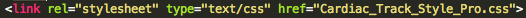
\includegraphics[width=\linewidth]{csslink.png}
\caption{Calling CSS script \label{csslink}}
\endminipage\hfill
\minipage{0.19\textwidth}
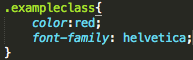
\includegraphics[width=\linewidth]{exampleclass.png}
\caption{CSS example \label{CSSex}}
\endminipage
\end{figure} 
The general format of a .css file is shown in fig.\ref{CSSex}, in this example the "exampleclass" denotes which class in the html is being formatted, "." is used to prefix a class and "\#" an id. Within the "\{\}" brackets are the commands, here the font is made red and in the Helvetica style. The style sheet is called cascading because any div's that are contained within other div's inherit the style of the parent div they are contained within. The CSS is also used for the positioning, and size of all divs. 

\subsubsection{JavaScript and JQuery}
JavaScript facilitates dynamic functions to be performed within the browser. "jQuery is a fast, small, and feature-rich JavaScript library. It makes things like HTML document traversal and manipulation, event handling, animation, and Ajax much simpler with an easy-to-use API that works across a multitude of browsers." \cite{Jquery}. Javascript is specifically used in this website to form the tutorial, graph, the uncertainty bar and the patient selector. It should be noted that because the functions are performed within the user's browser it is not trivial to pass variables between JavaScript and PHP which is conversely run on the server side of the website. 

%%%%%%%%%%%%%%%%%%%%%%%%%%%%%%%%%%%%%%%%%%%%%%%%%%%%%%%%%%%%%%%%%%%%%%%%%%%%%%%%%%%%%%%%%%%%%%%%%%%%%%%%%%

\section{Patient Application - \textit{Michael Fedosiuk}}

The key goal for the patient application was usability. Due to hypertension mainly affecting those over 50 years of age, this is the target audience of the application. Firstly simplicity is key, uncluttered pages with distinct labelled buttons where possible. Secondly both font and button size need to be large, to account for loss of vision and dexterity in some users. 

\begin{wrapfigure}{l}{.73\textwidth}
\centering
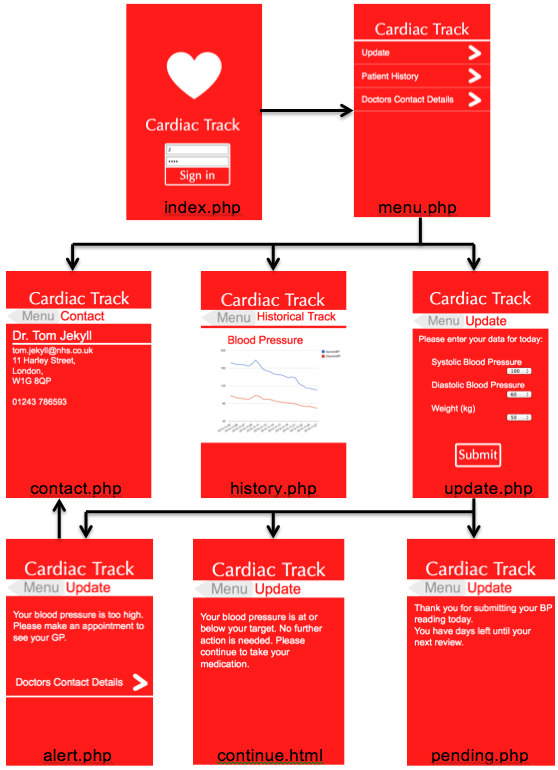
\includegraphics[width=1\linewidth]{patientUI.png}
\caption{Patient UI journey walkthrough (page names shown in black at the bottom and refer to the following sections) \label{patientUI}}
\end{wrapfigure} 
Finally consistency between pages making learning to use the application easier and faster. The app's itself is written in PHP for all but one page, however most of the content of these files consist of html. The app has been optimised for use on iPhone 5 however will also function on an iPad and android phones with minimal scaling problems. All pages bar one are styled using the same CSS file "Cardiac\_Track\_Style.css" that is 297 lines long. 

\subsection{General format}
For consistency and efficiency of programming, most pages have the same standard format. Fig.\ref{appstandard} shows the PHP, HTML and CSS that together form the standard page, also shown.
\begin{figure}[h!] 
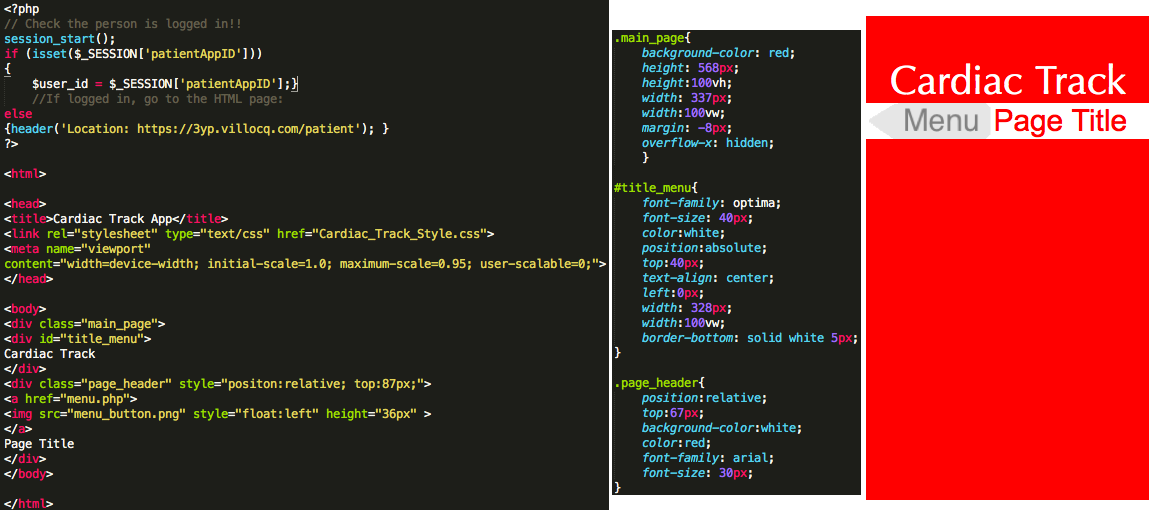
\includegraphics[width=\linewidth]{appstandard.png}
\caption{Left:php and html Middle: CSS Right: Standard app page \label{appstandard}}
\end{figure} 
The PHP script starts with a PHP function which checks if a user is logged in, if they are not it redirects them to the login page "https://3yp.villocq.com/patient". 
\\ \indent
The rest of the script is written in html between the $<$html$>$ tags. Firstly in the page header the title is set; this is displayed in the top of a web browser. The link to the CSS page is then made and finally within the head meta-properties for the viewport are set. The viewport properties affect how the site is shown on the device. The first term "width=device-width" means that the content of the page fills the device's screen, hence maximises the size of the content displayed. The "Initial-scale=1.0; maximum-scale=0.95; user-scalable=0;" means that when the page loads the page is scaled to the device width, and that the user is unable to zoom in or out of the page. Disabling the zoom function aids the application's usability as the page remains consistent when the user may accidentally tap the screen. 
\\ \indent
The first main div within the body of the page is given the class="main\_page", as seen in the CSS this sets the background of the app using the vh/vw units. Initially the app was programmed with the px unit (these has been left in for old browser compatibility), however they were updated to the new CSS 3 unit once they had been discovered for use in the currentpatients/index.php page. The benefit of their use in the patient app is that they provide greater device compatibility, as the app is now able to fill any screen. Before using the px unit meant the app specifically only fitted the screen of an iphone5. For further information on the scaling unit refer to the currentpatients/index.php, Page segments and scaling section. Finally the margin term is to remove the white edges which are automatically shown when a webpage is displayed and the "overflow-x:hidden" stops the page from moving when scroll selection in the update page is used. The "title\_menu" is what formats the white "Cardiac Track" title. The final div "page\_header" is what creates the white band at the top of the page. The "position:relative" which is seen throughout all CSS means that any positioning is done relative to the surrounding div's, the other option is to set "position:absolute" this means positioning is done relative to the edge of the page. Within the div the image "menu\_button.png", the grey button, which was drawn in Paint \cite{paint} is screened. This is linked to the "menu.php" page. The CSS for the menu button has been written with the html using style="float:left" this makes the button position itself to the far left of the div it is within. The pages based on this format are the same except the title and the additional content which is added between the final $<$/div$>$ and $<$/body$>$ tags. 

\subsection{patient/index.php}
The index.php page is the page to which all users are initially directed so they can login. It based around a JavaScript form (left fig.\ref{logincode}), of which the JavaScript function (top right fig.\ref{logincode}) is held in the page's head and the form itself is a table within the html. There is a specific JavaScript function "submitform" which extracts the data from the form specified, in this case with the id="jsform". The form seen in the html has the action="login.php" and method="post", this means that the data entered is sent to the script login.php. The $<$input$>$ tags set what the input type is (password turns the covers text after the next letter is entered), it also names the variable and states whether or not it is required for the form to be submitted. Finally to run the JavaScript and submit the form a link href="javascript: submitform()" is set for the submit button. 
\begin{figure}[h!] 
\centering
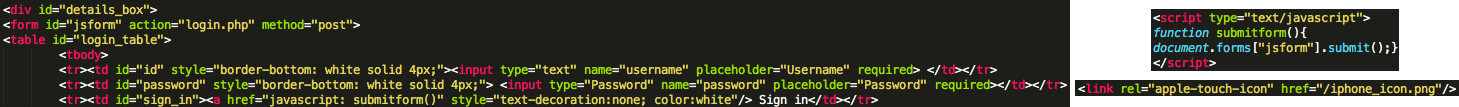
\includegraphics[width=1.0\linewidth]{logincode.png}
\caption{Left:html JS form Top Right:JavaScript function Bottom Right:Apple touch icon \label{logincode}}
\end{figure} 

\begin{wrapfigure}{l}{.14\textwidth}
\centering

\includegraphics[scale=0.07]{iphoneicon.png}
\caption{iPhone icon \label{iphoneicon}} 
\end{wrapfigure} 
Within the head of the html the code in the bottom right of fig.\ref{logincode} was added. This sets the "apple-touch-icon". If a user adds a link to the home screen of their iPhone or iPad, the link will take the form of the "iphone-icon.png". The icon has been created in Paint \cite{paint} and gives the link the look of a native application, fig.\ref{iphoneicon}. This enhances usability by making the login page easier to navigate to. 

\subsubsection{menu.php}
This is the page to which the patient is sent once they have logged into the app. It allows users access to any of the apps other pages. It is very simple in its construction simply screening the text and arrow images and sets the applicable href="..." tag to set the link it to the relevant page. 

\subsubsection{update.php}
\begin{wrapfigure}{r}{.35\textwidth}
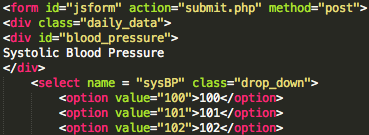
\includegraphics[width=1\linewidth]{updateform.png}
\caption{Update Systolic BP form \label{updateform}}
\end{wrapfigure} 
This is where the user comes to enter their BP measurement each day. The data is posted using the same JavaScript function, (top right of fig.\ref{logincode}) as the login page. However the location and the make up of the form are naturally different. Although as seen in the top line of fig.\ref{updateform}, the method="post" is the same as in the login page the action has change to "submit.php" which is where the update data is sent to be entered into the database. The form is a drop down menu which is created using the $<$select$>$ tags in conjunction with the $<$option$>$ tags. Within each tag the value="..." must be set as well as the option that is displayed. This is because it is the value not the option that is sent to the database. Options for systolic range from 100mmHg to 190mmHg (above 180mmHg is a hypertensive crisis) and for diastolic range from 60mmHg to 150mmHg, encompassing all possible measurements.

\subsubsection{Result pages}
On submitting the update form patients are direct to one of three pages (bottom fig.\ref{patientUI}) by the submit.php script dependant on what their current BP status is. The pages themselves are created from the general format shown at the start of this section. If the patient has had their medication reviewed within the last 28 days their BP may have not yet stabilised hence they are sent to the pending.php page. If they are below their target BP they are directed to the continue.html. If however they have breached their target BP they are sent to alert.php. This page provides a link to the contact.php page easing the process of booking an appointment. Note the link is in the same style as that on the menu page to preserve continuity. 

%\subsubsection{Contact.php}

\subsubsection{history.php}
 
\begin{wrapfigure}{r}{.5\textwidth}
\minipage{0.50\textwidth}
\centering 
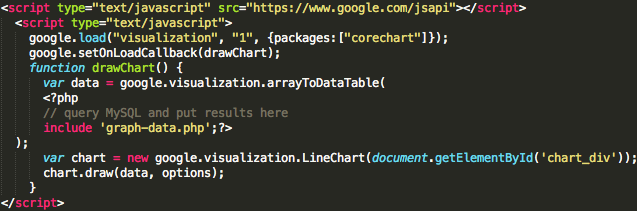
\includegraphics[width=0.95\linewidth]{historyJS.png}
\caption{JavaScript for graph creation \label{historyJS}}
\endminipage\hfill
\end{wrapfigure} 
This section can be accessed from the menu and allows the user to see how their BP has varied overtime. It has been added as an incentive to use the app. A line graph is created dynamically using Google charts \cite{chart} which is based in JavaScript. To use the Google JavaScript application-programming interface, it must first be imported which is done in the top line of fig.\ref{historyJS}. In the main script the required packages that draw the graph are loaded and then a function is created to set the details of the chart. The variable data is created and script, graph-data.php is used to query this data from the database and load it in the correct format. Finally the variable chart is used to set the type of graph and name the element in which the chart will appear on the page, "chart\_div". 

%%%%%%%%%%%%%%%%%%%%%%%%%%%%%%%%%%%%%%%%%%%%%%%%%%%%%%%%%%%%%%%%%%%%%%%%%%%%%%%%%%%%%%%%%%%%%%%%%%%%%%%%%

\section{Doctor's Application - \textit{Emma Saragossi}}

\subsection{Function}

The \textit{Cardiac Track Pro} doctor portal has three primary functions:
\begin{enumerate}
\item \textbf{Patient monitoring} - the doctor can view their existing patients' blood pressure and treatment history, and is alerted when their patient requires a check-up or treatment review.
\item \textbf{New patient creation} - the doctor can create a new patient profile, storing the patient history and target blood pressure levels.
\item \textbf{Treatment selection} - a treatment selection tool advises the doctor on the best course of treatment for the patient based on their medical history. It also determines when to schedule follow up appointments.
\end{enumerate}

\subsection{User interface}

The doctor application is to be viewed in a web browser. Web pages are built using two key technologies: HTML (the Hypertext Markup Language) and CSS (Cascading Style Sheets). The HTML provides the structure of the page while CSS provides the layout and formatting. It is important to keep the page structure and design quite separate. This is because it allows all pages to share the same style sheet. The site is then easier to maintain, as only one file need be updated to change the appearance of the site.  In addition, CSS is much more flexible for specifying the design.

\subsubsection{General page structure - HTML}


\begin{code}[ht]
\begin{html}
<link href="styles/style.css" rel="stylesheet" type="text/css">
<body>

<div class="container">
  	<header><!--include header info here (logo, search bar)-->
    </header>
    
    <div class="sidebar">
    <nav><!--include navigation links here to internal pages-->
    </nav>
    </div>

    <div class="content"><!--include page content here-->
    </div>
  	
</div>

<footer class="footer"><!--include footer links here-->
	</footer>

</body>
\end{html}
\caption{General page format (HTML)}
\label{code:htmlGeneral}
\end{code}


The general format for the structure of each page is shown in Extract~\ref{code:htmlGeneral}. At the top of all HTML files is a link to the style sheet, the source of all page formatting. All page content, such as text, hyperlinks or images, must fall within HTML body tags. HTML div tags are then used to separate the page content. Div tags define sections in an HTML document, and group block elements so that they can be formatted with CSS.

Standard to all pages is the header, sidebar, page content and footer. The header will contain the site logo, and a search bar which will allow the user to search for a patient using their patient ID. The sidebar will display the links which allow the user to navigate around the site, as well as a news feed, which will alert the user to any patients who are not at their target blood pressure. The footer contains more navigation links (e.g. Site Terms, About Us page). The page content div is standard to all pages, but what is placed within it changes depending on the purpose of the page.

The header, sidebar and page content are all held within a div called container. This is useful when it comes to formatting the page (see Section~\ref{sec:CSS}).

\subsubsection{Optimizing layout for multiple browser dimensions}
\label{sec:CSS}
It is unlikely that the doctor will view the site on a mobile device. The decision was made, therefore, to focus on optimizing the display for desktop and tablet web browsers.

A standard tablet display is 768 x 1024px, while typical desktop displays are much wider. If the site is viewed with the tablet in landscape, the page content must be limited to 1024px in width, while the height of the page can be unlimited. This ensures that the user will only have to scroll down the page, and not across, to view content, making the site more user-friendly on tablet devices. The decision was made to limit the width of all page content to 960px to fit comfortably within the 1024px limit, so that the site may be compatible with as many browser dimensions as possible.

The width of the browser should therefore be greater than the width of the page content. The CSS, shown in Extract~\ref{code:cssGeneral}, formats the page such that all content is centred in the browser, no matter what the browser width, leaving a margin either side of the page content. In the HTML, the bulk of the page content is held in the container div. In the CSS, the margins of the container are set to auto. This automatically centers the container div, and anything within it. Figure~\ref{fig:pageLayout} shows the layout set by the CSS, and where the div elements sit in relation to the browser and each other.


\begin{code}[ht]
\begin{css}
@charset "utf-8";
*{
}
html, body {
	height: 100%;
    /*body and html fill entire browser height*/
}
body {
	background-color: #F1F1EF;
	margin: 0;
	padding: 0;
    /*body colour is pale grey and has no margin (fills browser width)*/
}
.container {
	min-height:100%
	height: auto!important;
	width: 960px;/*container is white and width limited to 960px */
	background-color: #FFFFFF;
	margin: 0 auto -4em;/*no margin at top. auto margin on sides. bottom margin sits 4em from bottom.*/
	padding-bottom: 40px;
    
}
header {
	width: 960px;
}
.sidebar1 {
	float: left;/*sidebar sticks to left of page content*/
	width: 200px;
	height: auto;
}
.content {
	width: 760px;
	float: right;/*page content floats to right of sidebar*/
	height: auto;
}
.footer {
	height: 4em;
	clear: both; /*clear - no floating elements allowed either side*/
	width: 960px;
	margin-left: auto;
	margin-right: auto;
	position: relative;/*centers footer immediately below container*/
}
\end{css}
\caption{CSS for page layout}
\label{code:cssGeneral}
\end{code}


\begin{figure}[ht]
\begin{center}
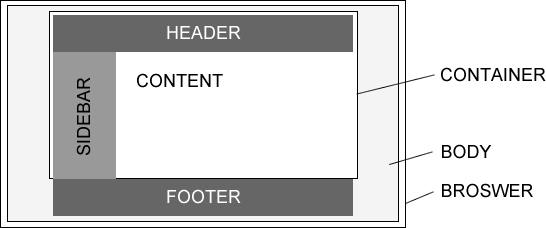
\includegraphics[scale=0.5]{pageLayout}
\caption{Layout of HTML div elements}
\label{fig:pageLayout}
\end{center}
\end{figure}

%\subsubsection{Footer??}
%em: unit equal to the computed value of the font size property of the element on which it is used.
%container ends 4em from bottom of page - allow room for footer.

\subsubsection{Text formatting}

As well as defining the layout of the HTML elements, the CSS also provides the site's text formatting and colour profiles.

The typeface used for the site is Helvetica, an easy to read sans-serif font which is commonly found installed on most devices. A font-family was defined in the CSS to include both Helvetica and Arial. If for some reason the browser used to view the site does not support Helvetica, the browser will display all text in the fallback font, which is Arial.

All text included in the page content is set to be black with a regular weight, apart from any text which serves as a hyperlink (which is defined in the HTML). To distinguish a hyperlink from plain text, a rule was created within the CSS to underline links and display them in bold. In addition, if a user scrolls over a link with their cursor, the link changes colour.

\subsubsection{Logo image}
The logo in the header (seen in Figure~\ref{fig:siteDesignGeneral}) was created as an image rather than displayed as live text on the site in order to preserve the appearance of the logo design. This is because the font chosen for the logo, Optima, does not come installed as standard on devices. If a visitor to the site does not have Optima installed, their browser would select an alternative font.

The image was saved as a Portable Network Graphic (PNG), a raster graphics file format that supports lossless data compression. Raster graphics images are dot matrix data structures representing a grid of pixels, unlike vector graphics which comprise of paths and are defined by a start and end point. Vector images are often considered the first choice for logos, as they can be scaled easily. If you try to enlarge a raster image, the image edges get jagged as you enlarge them. However, the most common vector graphic file format, SVG (Scalable Vector Graphic), is not well supported by desktop and mobile browsers \cite{SVG}. As the logo is only to be viewed digitally and does not need to be scaled, a raster image format was therefore considered acceptable.

\begin{figure}[ht]
\begin{center}
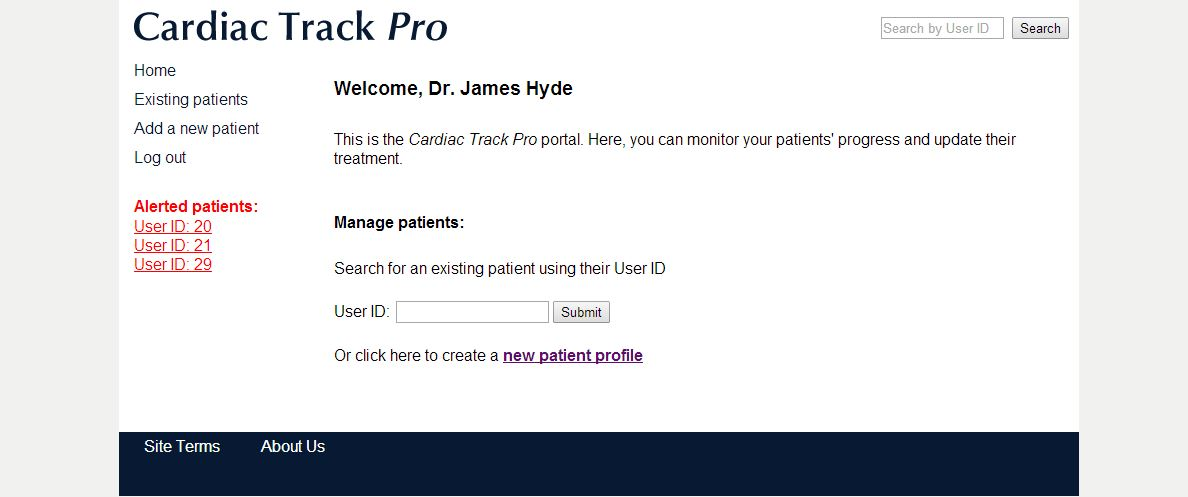
\includegraphics[scale=0.5]{siteDesignGeneral}
\caption{Example page layout - \textit{About Us} page}
\label{fig:siteDesignGeneral}
\end{center}
\end{figure}

\subsection{User access}

\subsubsection{Login page}
A login page for the doctor portal is required to grant the user access to the internal pages of the site, and to prevent others from viewing or altering sensitive data. It also ensures that only relevant data is displayed to the user. Access is controlled by identifying and authenticating the user. A PHP script is called to check the user’s credentials (username and password) and grant or deny access to the internal pages of the site.

The login page displays the Cardiac Track Pro logo and houses two text input boxes – one for the username and one for the password – and a submit button which will call the PHP script to check the login credentials when clicked.

\begin{figure}[ht]
\begin{center}
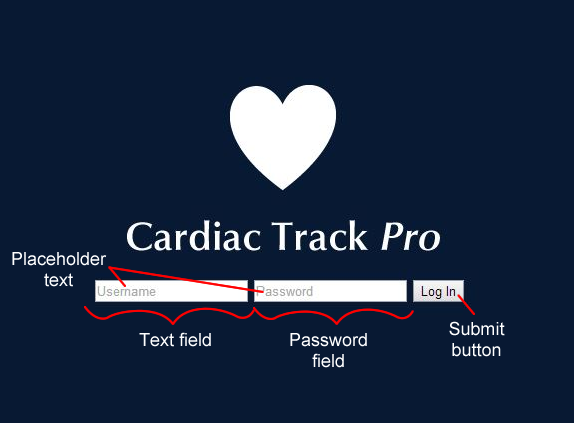
\includegraphics[scale=0.6]{login_design}
\end{center}
\caption{Login page appearance}
\label{fig:login_design}
\end{figure}

An HTML form was created to send the login data to the server (see Extract~\ref{code:loginHtml}).

\begin{code}[ht]
\begin{html}
<form action="login.php" method="post">
	<input type="text" name="username" placeholder="Username">
	<input type="password" name="password" placeholder="Password"> 
	<input type="submit" value="Log In" name="formSubmit">  
</form>
\end{html}
\caption{HTML form for login credentials}
\label{code:loginHtml}
\end{code}


The METHOD attribute of the FORM element specifies the HTTP method used to send the form to the processing agent. There are two commonly used methods for a request-response between a client and server: GET and POST. The GET method encodes the form data into the URL, while the POST method hides the data in the message body meaning it cannot be seen by the user. POST requests cannot be cached or bookmarked and do not remain in the browser history. Due to the sensitive nature of the form data, POST was chosen.

The TEXT and PASSWORD fields are standard HTML input elements for forms. The characters in a password field are automatically masked (shown as asterisks) for security. The PLACEHOLDER attribute specifies the expected value of an input element (see Figure~\ref{fig:login_design}). The SUBMIT button sends the form data to the server. The data is sent to the page specified in the form's ACTION attribute - here it calls the PHP script \textbf{login.php} (See section \ref{drloginform})


\subsubsection{Internal pages}

A user must only be granted access to the internal pages of the site if they have already logged in i.e. a user cannot gain access to the internal pages of the site by simply entering the page URL. A PHP script is included at the top of all internal pages which checks whether the user has logged in successfully and is authorised to view the page content. Otherwise, the user is redirected to the login page. The code is shown in Extract~\ref{code:intPages}

The user ID was stored as a session variable in \textbf{login.php}. Session variables (see section \ref{phpsessions}) store information about a single user and make it available to all pages of the site. These are temporary and are deleted after the user logs out or closes their browser. The isset() function checks whether the session variable \mbox{\$\_SESSION['userID']} has already been set. This will only be true if the user has logged in successfully previously. If the variable has not been set, the user has not been granted access, and is redirected to the login page.


\begin{code}[ht]
\begin{php}
<?php

// Check the person is logged in!
session_start();    
if (isset($_SESSION['userID'])) $
{
    //Continue to the page
    // This sets the current user ID as php variable!
    $doctorID = $_SESSION['userID'];
}
else
{
    //Login Failure
header('Location: https://3yp.villocq.com/doctor/loginPage.php'); 
}
?>
\end{php}
\caption{Internal pages - security}
\label{code:intPages}
\end{code}


\subsection{Creating a patient profile}

Relevant information about the patient needs to be uploaded and saved to the database. This information is required to determine the patient's target blood pressure, and is used by the Tallis treatment tool to determine the best course of drug treatment for the patient.

Initially, the data was entered, and the target blood pressure calclulated, within the Tallis application. However for design reasons this was later removed and implemented separately.

\subsubsection{Initial design}

The initial design used Tallis to implement the enquiry and decision process. Tallis "is a suite of software tools to support authoring, publishing and enacting of clinical knowledge applications over the web" \cite{tallisDescription}. The software is built around PRO\textit{forma}, a language designed to model clinical processes. PRO\textit{forma} supports top down design. A defined set of tasks is mapped out into a network of plans and procedures. This represents the high-level structure of a guideline. 

\begin{figure}[ht]
\begin{center}

\includegraphics[scale=0.8]{tallis_keystone_top}
\caption{Top level design - keystones}
\label{fig:tallis_keystone_top}
\end{center}
\end{figure}

Tasks are initially represented as keystones. Keystones represent a generic task. These are later converted into a specific task - either a plan, decision, enquiry or action. Plans can contain a series of tasks within them. The initial keystone layout for the hypertension treatment tool is shown in Figure~\ref{fig:tallis_keystone_top}, and is based on NICE Clinical Guideline 127 \cite{CG127}. The set of tasks is as follows:
\begin{enumerate}
\item \textbf{Disclaimer} - NICE Clinical Guideline 127 offers guidance on the treatment of primary hypertension in adults. The \textit{disclaimer} task makes the doctor aware of the scope of the application. The application is not suitable for:
\begin{itemize}
	\item hypertension in children
	\item hypertension in pregnancy
	\item hypertension in patients with diabetes
	\item specialist management of secondary hypertension
	\item specialist management of hypertensive crises
\end{itemize}
The keystone becomes an \textit{enquiry}. A series of questions are posed to the user to determine whether the patient is suitable. The questions are posed such that if the answer is "Yes" the patient is unsuitable. For example, "Is the patient pregnant?". If the answer to any of the questions is "Yes", the next task implemented is an \textit{action} informing the doctor that the patient does not meet the scope of the application, and the process is then terminated. If the answer to all of the questions is "No", the process continues to the \textit{Patient data} task.

\item \textbf{Patient data} - here, the doctor enters all relevant information about the patient's background and medical history. This keystone becomes a plan, containing a series of enquiries about the patient (see Figure~\ref{fig:tallis_plan_patientdata}). This was represented as series of enquiries rather than one single enquiry for two reasons. The first is that it splits up the patient data entered by type. The second is that it allows an additional line of questioning to be offered to a subset of patients. Within the \textit{Patient details} enquiry, the doctor is required to enter the gender of the patient. A secondary enquiry is then only offered if the patient is female.

\begin{figure}[ht]
\begin{center}
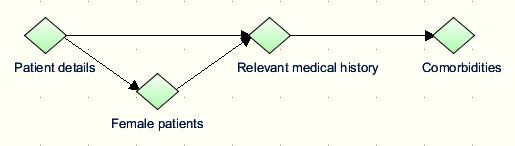
\includegraphics[scale=0.8]{tallis_plan_patientdata}
\caption{Patient data enquiry}
\label{fig:tallis_plan_patientdata}
\end{center}
\end{figure}

\item \textbf{Target blood pressure} - this determines the patient's target blood pressure. Target blood pressure is based on the patient's age and whether or not they have been diagnosed with 'white coat' hypertension\footnote{Patient exhibits elevated blood pressure in a clinical setting but not in other settings, often due to anxiety}. These are known from the \textit{patient data enquiry}. The keystone becomes a \textit{decision} task. A \textit{decision task} "defines the decision options, relevant information and a set of argument rules which determine which of the options should be chosen according to current data values" \cite{tallisDecision}. There are four candidates for the target blood pressure, each with two arguments (see Table~\ref{table:targetBP}). In the argument column, (--) means exclude this candidate if the source meets a particular argument. For example, if the candidate has 'white coat' hypertension, their target blood pressure cannot be 140/90mmHh or 150/90mmHg.
\begin{table}[ht]
\begin{center}
\begin{tabular}{|p{1.8cm}|p{1.5cm}| l | l |p{3.5cm}|}
\hline
\textbf{Candidate name} & \textbf{Target BP (mmHg)} & \textbf{Argument 1} & \textbf{Argument 2} & \textbf{Description} \\
\hline
Systolic140 & 140/90 & Whitecoat="Yes" (--) & Age\_group="80+" (--) & Patient must not have white coat hypertension AND be younger than 80 years of age \\
\hline
Systolic150 & 150/90 & Whitecoat="Yes" (--) & Age\_group!="80+" (--) & Patient must not have white coat hypertension AND be younger than 80 years of age \\
\hline
Systolic135 & 135/85 & Whitecoat="No" (--) & Age\_group="80+" (--) & Patient must not have white coat hypertension AND be younger than 80 years of age \\
\hline
Systolic145 & 145/85 & Whitecoat="No" (--) & Age\_group!="80+" (--) & Patient must not have white coat hypertension AND be younger than 80 years of age \\
\hline
\end{tabular}
\caption{Decision logic for determining target blood pressure in Tallis}
\label{table:targetBP}
\end{center}
\end{table}

\item \textbf{Treatment selection} - this chooses the drug treatment for the patient (see Section~\ref{sec:Treatment} for more detail).
\end{enumerate}

The network of specific tasks, shown in Figure~\ref{fig:tallis_task_top}.

\begin{figure}[ht]
\begin{center}
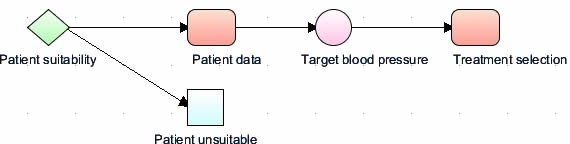
\includegraphics[scale=0.8]{tallis_task_top}
\caption{Top level design with specific tasks populated}
\label{fig:tallis_task_top}
\end{center}
\end{figure}


\begin{comment}
Patient suitability enquiry
Aim – terminates process early if patient is unsuitable  doctor avoids entering all patient info before finding out patient is unsuitable
Scope as defined by NICE guidelines

\begin{center}
\begin{tabular}{| l | l | l | l |}
\hline
Name & Data Definition & Status	& Caption \\
\hline
Age\_young & booleanType & Mandatory & Is the patient under 18 years of age? \\
\hline
Crisis & booleanType & Mandatory & Is the patient in a state of hypertensive crisis? \\
\hline
Diab & booleanType & Mandatory & Has the patient been diagnosed with Type I or Type II diabetes? \\
\hline
Preg & booleanType & Mandatory & Is the patient pregnant? \\
\hline
Second & booleanType & Mandatory & Has the patient been diagnosed with secondary hypertension? \\
\hline

    \end{tabular}
\end{center}

Mandatory status – question must be answered for process to continue
No need to follow this with a decision task to determine whether patient is suitable
Patient unsuitable precondition – if answer to any of the above is "Yes"
	Displays text alerting doctor that patient is unsuitable
	Process is then terminated
Patient data precondition – if answer to all of above is "No"

Patient data plan enacted only if patient is eligible
Series of enquiries – patient details (age, gender, ethnicity etc)
If female, further line of questioning regarding pregnancy and breastfeeding
	Precondition set that Gender = 
	"Female"
Otherwise, process continues to comorbidities - the presence of one or more additional disorders (or diseases) co-occurring with a primary disease or disorder; or the effect of such additional disorders or diseases. This will heavily influence the appropriate choice of treatment (contraindications)
\end{comment}


Figure~\ref{fig:Tallis_UI_unsuitable} shows the Tallis User Interface (UI) for an \textit{enquiry} task. Radio buttons are used to enter patient data. They are presented in two columns, meaning the information is not easy to digest. We decided to update the UI to make data entry as efficient and easy for the user as possible. It was at this point that the decision to split the application was made: the treatment selection would still take place in Tallis, but the patient data would be entered into a separate web form and then submitted to the database. This is because creating an HTML form is quite straightforward. Moreover, we would have more control over the UI if we built our own site.

As the target blood pressure decision task had relatively few candidates and arguments, it was also decided that this would be removed from the Tallis application, and instead the target blood pressure would be determined in a PHP script.

\begin{figure}[ht]
\begin{center}
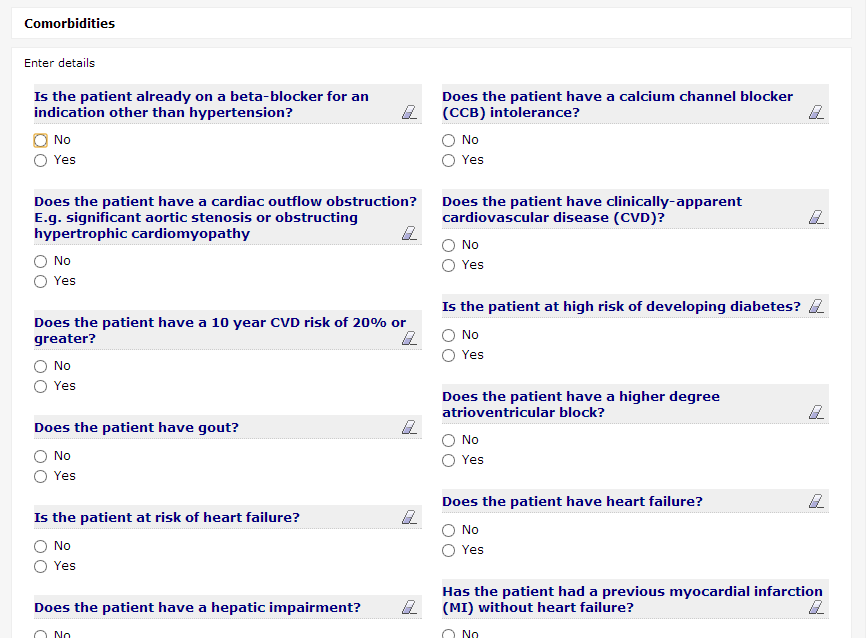
\includegraphics[scale=0.7]{Tallis_UI_unsuitable}
\caption{Current UI for Tallis enquiry task}
\label{fig:Tallis_UI_unsuitable}
\end{center}
\end{figure}

\subsubsection{Separate patient creation form}

An online tool was created to allow the doctor to add a new patient to the database. A series of HTML forms allows the doctor to enter relevant information about their patient. Each form requires the doctor to enter a different class of information (for example one form for medical history, a second form for comorbidities etc.). Each form appears on a different web page. The first form must be completed to be able to continue to the next.

The data is not saved to the database with each separate page. This would be more difficult than executing just one SQL command to submit ALL the data to the database in one go. For example, if the doctor clicks submit on the first page, but then doesn’t continue, half of the data will exist in the database but some of it will be missing. Rather than each page submitting to the database, each form variable is stored as a SESSION variable. Session variables are saved locally between pages but are not yet stored in the database. Once the doctor has completed all the forms, the final form submit button will call a PHP script which will assign all the session variables as PHP variables and save them to the database.
\begin{enumerate}
\item \textbf{Disclaimer}

The first form is similar to the \textit{Disclaimer} enquiry from the initial Tallis application. It terminates the patient creation process if the patient does not meet the scope of the clinical guideline. The form can be seen in Figure~\ref{fig:formCheckBox}, and constists of a series of checkboxes. The HTML for creating a checkbox element in a form is shown in Extract~\ref{code:checkBox}.

\begin{figure}[ht]
\begin{center}
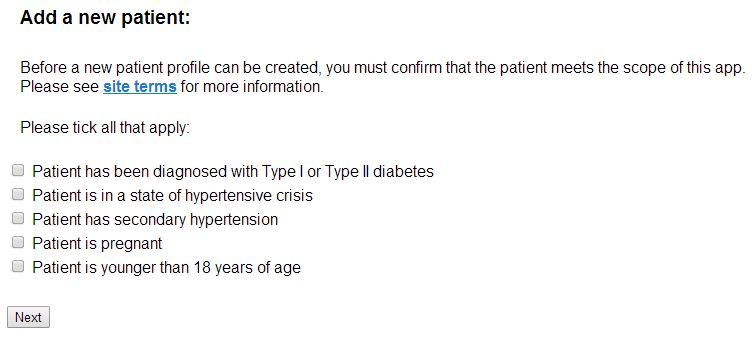
\includegraphics[scale=0.5]{formCheckBox}
\caption{Current UI for check box form}
\label{fig:formCheckBox}
\end{center}
\end{figure}


\begin{code}[ht]
\begin{html}
<form id="suitability" action="suitable.php" name="suitability" method="post">
  <table width="540">
     <tr>
     <td><label><input type="checkbox" name="A" value="A" id="diabetes">
     Patient has been diagnosed with Type I or Type II diabetes</label></td>
     </tr>
     <!--repeat format (other questions)-->
  </table>

  <section id="submit">
  <input type="submit" name="next" id="next" value="Next">
  </section>
</form>
\end{html}
\caption{HTML - checkbox form}
\label{code:checkBox}
\end{code}


The checkbox inputs and their labels were entered into an HTML table to keep them aligned and make the form as efficient and easy to use as possible. The ACTION of the form calls the PHP script \textbf{suitable.php}, shown in Extract~\ref{code:phpTerminate}. This determines whether the patient meets the scope of the clinical guideline. If any of the checkboxes are selected, the patient is not suitable, and the doctor is redirected to a page indicating as such. This is done using the PHP function empty(), which determines whether a variable is considered to be empty i.e. it does not exist or if its value equals FALSE. If a checkbox is not selected, its value reads as FALSE. If none of the checkboxes are selected, the patient must be suitable, and is redirected to the next page in the patient creation process. 


\begin{code}[ht]
\begin{php}
<?php

$selectedA = $_POST['A'];
$selectedB = $_POST['B'];
$selectedC = $_POST['C'];
$selectedD = $_POST['D'];
$selectedE = $_POST['E'];

if(!empty($selectedA) or !empty($selectedB) or !empty($selectedC) or !empty($selectedD) or !empty($selectedE))
{
header('Location: https://3yp.villocq.com/doctor/newPatientUnsuitable.php'); 
}
else
{
header('Location: https://3yp.villocq.com/doctor/newPatientDetails.php'); 
}

?>
\end{php}
\caption{PHP for terminating process}
\label{code:phpTerminate}
\end{code}


\item \textbf{Entering patient data}

As an example, the form requiring the doctor to enter the patient's comorbidities is shown in Figure~\ref{fig:comor}. Patient details are entered into forms with radio box elements. Again, these are stored in an HTML table to align all radio boxes and text for comfortable viewing. The default value of all radio boxes is set to "No", so that the doctor is only required to if the patient has a condition.

\begin{figure}[ht]
\begin{center}
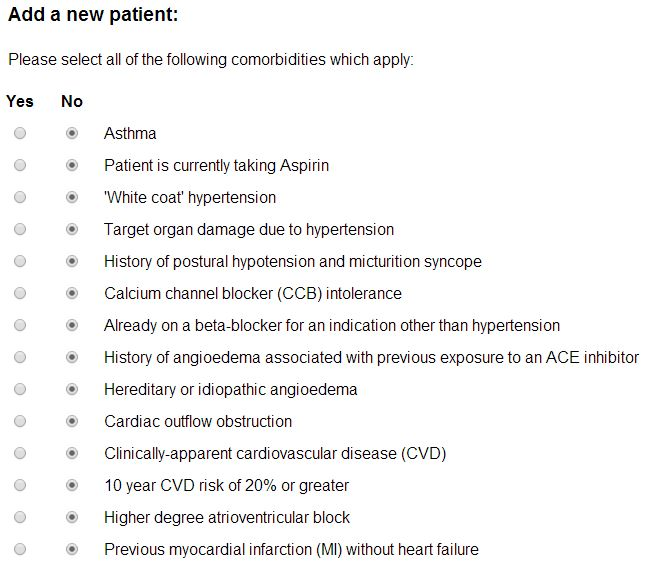
\includegraphics[scale=0.8]{comorbidity}
\caption{UI for radio box form}
\label{fig:comor}
\end{center}
\end{figure}

The HTML for creating a radio box form is shown in Extract~\ref{code:radioBox}. The ACTION for this form calls the PHP script \textbf{comorbidity.php} (Extract ~\ref{code:phpSession}). This assigns all the form variables to SESSION variables, as described earlier. It then redirects the user to the next page.


\begin{code}[ht]
\begin{html}

<form method="post" action="comorbidity.php">
      <table width="718" border="0" cellpadding="5">
        <tr>
          <td width="40" align="center"><strong>Yes</strong></td>
          <td width="40" align="center"><strong>No</strong></td>
          <td width="600"></td>
        </tr>
        
        <tr>
          <td align="center"><input name="Asthma" type="radio" value="Yes"></td>
          <td align="center"><input name="Asthma" type="radio" value="No" checked></td>
          <td>Asthma</td>
         </tr>
         <!--repeat: other comorbidities-->
         </table>
      
  <br>
  <input type="submit" name="formSubmit" value="Submit">
</form>
\end{html}
\caption{HTML for radio box enquiry}
\label{code:radioBox}
\end{code}

\begin{code}[ht]
\begin{php}
<?php

session_start();

if($_POST['formSubmit'] == "Submit")

{
	$_SESSION['asthma'] = $_POST['Asthma'];

}

header("Location: newPatientTargetBP.php");

?>
\end{php}
\caption{PHP - storing form data as session variables}
\label{code:phpSession}
\end{code}


\item \textbf{Determining target blood pressure}

In the initial Tallis design, a \textit{decision} task implemented the decision logic for determining the patient's target blood pressure. This is now implemented in the PHP script \textbf{target.php} instead, (see Extract~\ref{code:phpTargetBP}). There are two separate blood pressure values which need to be determined: the systolic and diastolc blood pressures. These are assigned empty PHP variables at the start of the script for efficiency. These are then determined as before; for example, if a patient is over 80 years of age AND has 'white coat' hypertension, their target blood pressure is 145/85mmHg. The target values are then stored as SESSION variables for later submission to the database. 


\begin{code}[ht]
\begin{php}
<?php

session_start();

$targetSystolic = "";
$targetDiastolic = "";

if ($_SESSION['ageGroup'] == "80+" AND $_SESSION['Whitecoat'] == "Yes")
{
$targetSystolic = "145";
$targetDiastolic = "85";
}

elseif ($_SESSION['ageGroup'] == "80+" AND $_SESSION['Whitecoat'] == "No")
{
$targetSystolic = "150";
$targetDiastolic = "90";
}


elseif ($_SESSION['ageGroup'] != "80+" AND $_SESSION['Whitecoat'] == "Yes")
{
$targetSystolic = "135";
$targetDiastolic = "85";
}

else
{
$targetSystolic = "140";
$targetDiastolic = "90";
}

$_SESSION['targetSystolic'] = $targetSystolic;
$_SESSION['targetDiastolic'] = $targetDiastolic;

?>
\end{php}
\caption{PHP for determining target blood pressure}
\label{code:phpTargetBP}
\end{code}


The target blood pressure needs to be displayed to the doctor for their own records. This is achieved by including the PHP echo() function within the page HTML (see Extract ~\ref{code:dispBP}). The PHP script \textbf{target.php} which determined the target value is included within PHP tags, and the SESSION variables assigned to the two target blood pressure values are echoed within the page content.


\begin{code}[ht]
\begin{html}
<?php include 'target.php' ?>
<h3>Add a new patient:</h3>
<p>We have calculated an appropriate target blood pressure for your patient, based on the patient information provided.</p>
<p>
Target systolic blood pressure:<strong><?php echo $_SESSION['targetSystolic'] ?>mmHg</strong>
<br>
Target diastolic blood pressure:<strong><?php echo $_SESSION['targetDiastolic'] ?>mmHg</strong>
</p>

\end{html}
\caption{Displaying target blood pressure to user}
\label{code:dispBP}
\end{code}

  
\item \textbf{Saving form data to database}

Once all forms have been completed and all form variables assigned to SESSION variables, the data can all be uploaded to the database. When the SUBMIT button of the final form is pressed, it calls the PHP script \textbf{submitAll.php}. An excerpt from this script is shown in Extract~\ref{code:submitAll}. First, all SESSION variables are assigned to PHP variables. The MySQL connection parameters are then configured and a new MySQL instance is created. The values are then bound and executed to the appropriate table within the database. 


\begin{code}[ht]
\begin{php}
<?php

session_start();

if($_POST['formSubmit'] == "Submit")

//Assign the creation form SESSION output to PHP variables
//Patient Details
$patientID = $_SESSION['patientID'];

//Repeat for others

// Configure the MySQL connection
$server="remote.villocq.com";
$username="3yp";
$DBpassword="project";
$database="tallis";

// New MySQLi Instance
$db = new mysqli($server,$username,$DBpassword,$database);

//Prepared statement:
$newPatient = $db->prepare("INSERT INTO patientInfo VALUES('')";

//Bind & Execute to submit to database. 
$newPatient->bind_param('s',$patientID);
$newPatient->execute();
$newPatient->close();
//Data has now been submitted to the database
//All records have now been created
?>
\end{php}
\caption{Submitting all data to database}
\label{code:submitAll}
\end{code}


\end{enumerate}

\subsection{News feed}
A news feed is displayed in the sidebar to flag for the doctor any alerted patients; that is, any patient who is not at their target blood pressure. The feed lists all alerted patients by their patient ID. The patient ID serves as a link which the doctor can click to take them straight to that patient's summary page, where they can then view the patient's blood pressure and medication history. 

The PHP function \textbf{patientsidebar} which generates the news feed is shown in Extract~\ref{code:PHPsidebar}. The function first connects to the database. Once the MySQL connection parameters have been configured and a new MySQL instance has been established, the alerted patients are identified by their patient ID (PHP variable: \textbf{id}). Alerted patients are all those in the table \textbf{patientInfo} whose blood pressure is not controlled and whose doctor is identified by the function parameter \textbf{\$doctorID} (the doctor currently logged in to the site).

The patient ID is then displayed to the user using the PHP echo() function. The HTML tag <a> indicates that the text is a hyperlink, while the href attribute specifies the link's destination. The URL to access the patient summary page is formulated such that the patient ID is embedded within the URL.


\begin{code}[ht]
\begin{php}
function patientsidebar($doctorID){
    
    // Configure the MySQL connection
    $server="remote.villocq.com";
    $username="3yp";
    $DBpassword="project";
    $database="tallis";
    
    // New MySQLi Instance
    $db = new mysqli($server,$username,$DBpassword,$database);
    
    $alerted = $db->prepare("SELECT id FROM patientInfo WHERE BPcontrolled='No' AND doctorID=?");
    $alerted->bind_param('s',$doctorID);
    $alerted->execute();
    $alerted->bind_result($id);
        
    while($alerted->fetch())
    {
        echo "<a href='https://3yp.villocq.com/doctor/currentpatients/index.php?w1=$id'>User ID: $id</a>";
        echo "<br>";
    }

    $alerted->close();
    $db->close();
}
\end{php}
\caption{patientsidebar PHP}
\label{code:PHPsidebar}
\end{code}


%%%%%%%%%%%%%%%%%%%%%%%%%%%!!!!!!!!!!!!!!!!!!!!!!!!!!!!!!!!!!!!!!!!!!!!!!!!!!!!!!!!!!!!!!!!!!!%%%%%%%%%%%%%%%%%%%%%%%%%%%%%%%%%%%%%%%%%%%%%%%
\subsection{Patient search bar}

Embedded in the header on all pages is the patient search bar, which allows the doctor to search by patient ID for immediate access to a patient's blood pressure and treatment history. As programmed within the currentpatients/index.php section, see for more detail on implementation. 

%An HTML form was created (Extract~\ref{code:searchBar}) which contains a standard TEXT input element and SUBMIT button. The form uses the GET method, which encodes the form data as a variable into the URL. When the SUBMIT button is pressed, the text entered into the TEXT element is appended to the link specified in the form's ACTION attribute and the page is redirected.


\begin{code}[ht]
\begin{html}
<form name="search" action="currentpatients/index.php" method="get">
<input type="text" name="w1" placeholder="Search by User ID" size="15">
<input type="submit" value="Search">
</form>
<!-- page will redirect to currentpatients/index.php?w1=id -->
\end{html}
\caption{HTML form for patient ID search bar}
\label{code:searchBar}
\end{code}

%%%%%%%%%%%%%%%%%%%%%%%%%%%!!!!!!!!!!!!!!!!!!!!!!!!!!!!!!!!!!!!!!!!!!!!!!!!!!!!!!!!!!!!!!!!!!!%%%%%%%%%%%%%%%%%%%%%%%%%%%%%%%%%%%%%%%%%%%%%%%

\subsection{Extension ideas for the Doctor Application}
At present, the prototype application only makes it possible for the doctor to create a new patient profile. It is perhaps desirable that the doctor should be able to edit this information if necessary. For example, a patient may develop new conditions which will need to be included as a patient comorbidity. Further work needs to be done, therefore, to allow the doctor to update and edit patient data.

\clearpage

%%%%%%%%%%%%%%%%%%%%%%%%%%%%%%%%%%%%%%%%%%%%%%%%%%%%%%%%%%%%%%%%%%%%%%%%%%%%%%%%%%%%%%%%%%%%%%%%%%%%%%%%%
\section{Doctor's Application - \textit{Michael Fedosiuk}}
\subsection{currentpatients/index.php}
\begin{figure}[h!] 
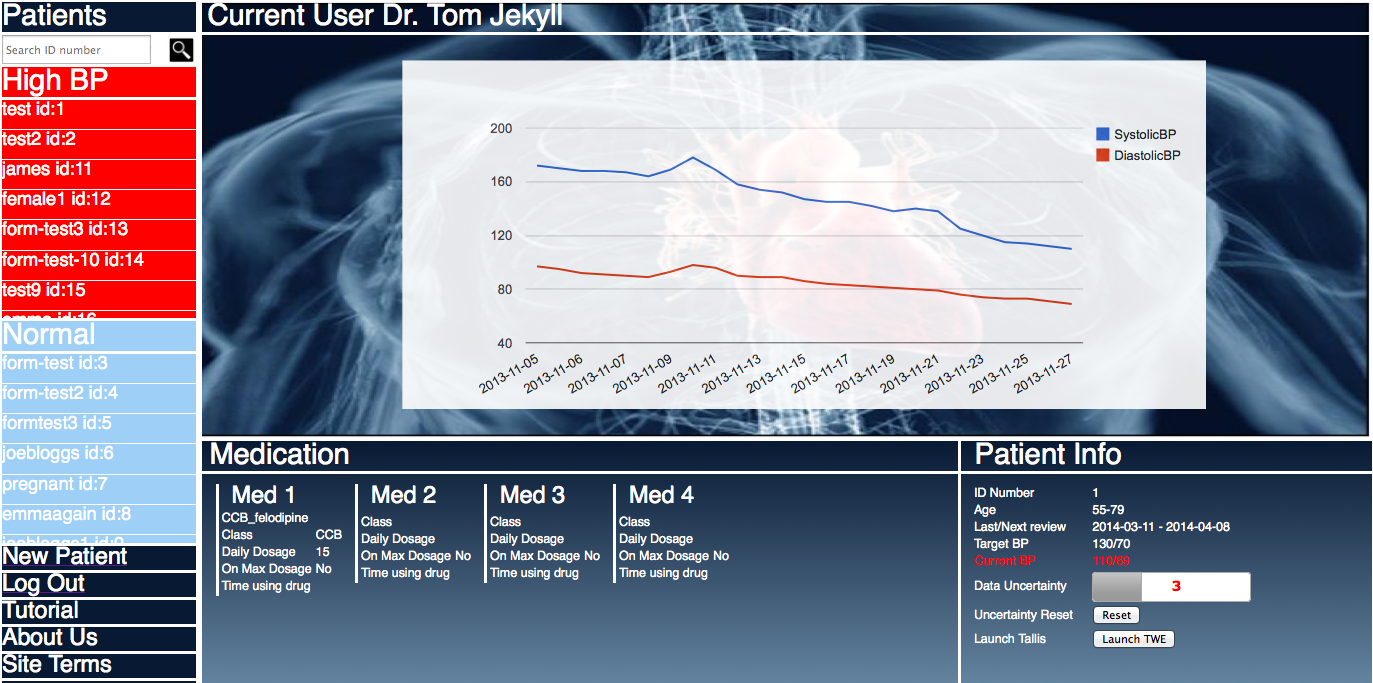
\includegraphics[width=\linewidth]{indexover.png}
\caption{The currentpatients/index.php page \label{indexover}}
\end{figure} 
\noindent 
Overview of index.php: It is a PHP file containing html, JavaScript, jQuery and SQL, it is 791 lines long. It is styled by the CSS file "Cardiac\_Track\_Style\_Pro.css", which is 835 lines long. 
\subsubsection{Page Segments and Scaling}
The page is created in 3 main div's, on the left, the patient selector, the top right the graph and the bottom is the patient information that is split between medication and personal information. The div's were created in the html and given different class names so they could be manipulated in CSS. 
\\ \indent
Originally the page scaling in the CSS was set using the \% unit, which sets the div to the stated \% of the viewport. The text within the div's was then set using the standard "font-size:20px", the px unit sets the size of the font by pixel number. 

\begin{wrapfigure}{l}{.34\textwidth}
\centering
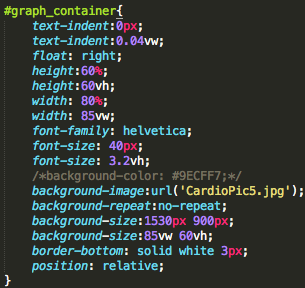
\includegraphics[scale=0.4]{CSSscaling.png}
\caption{Use of vh/vw scaling \label{CSSscaling}} 
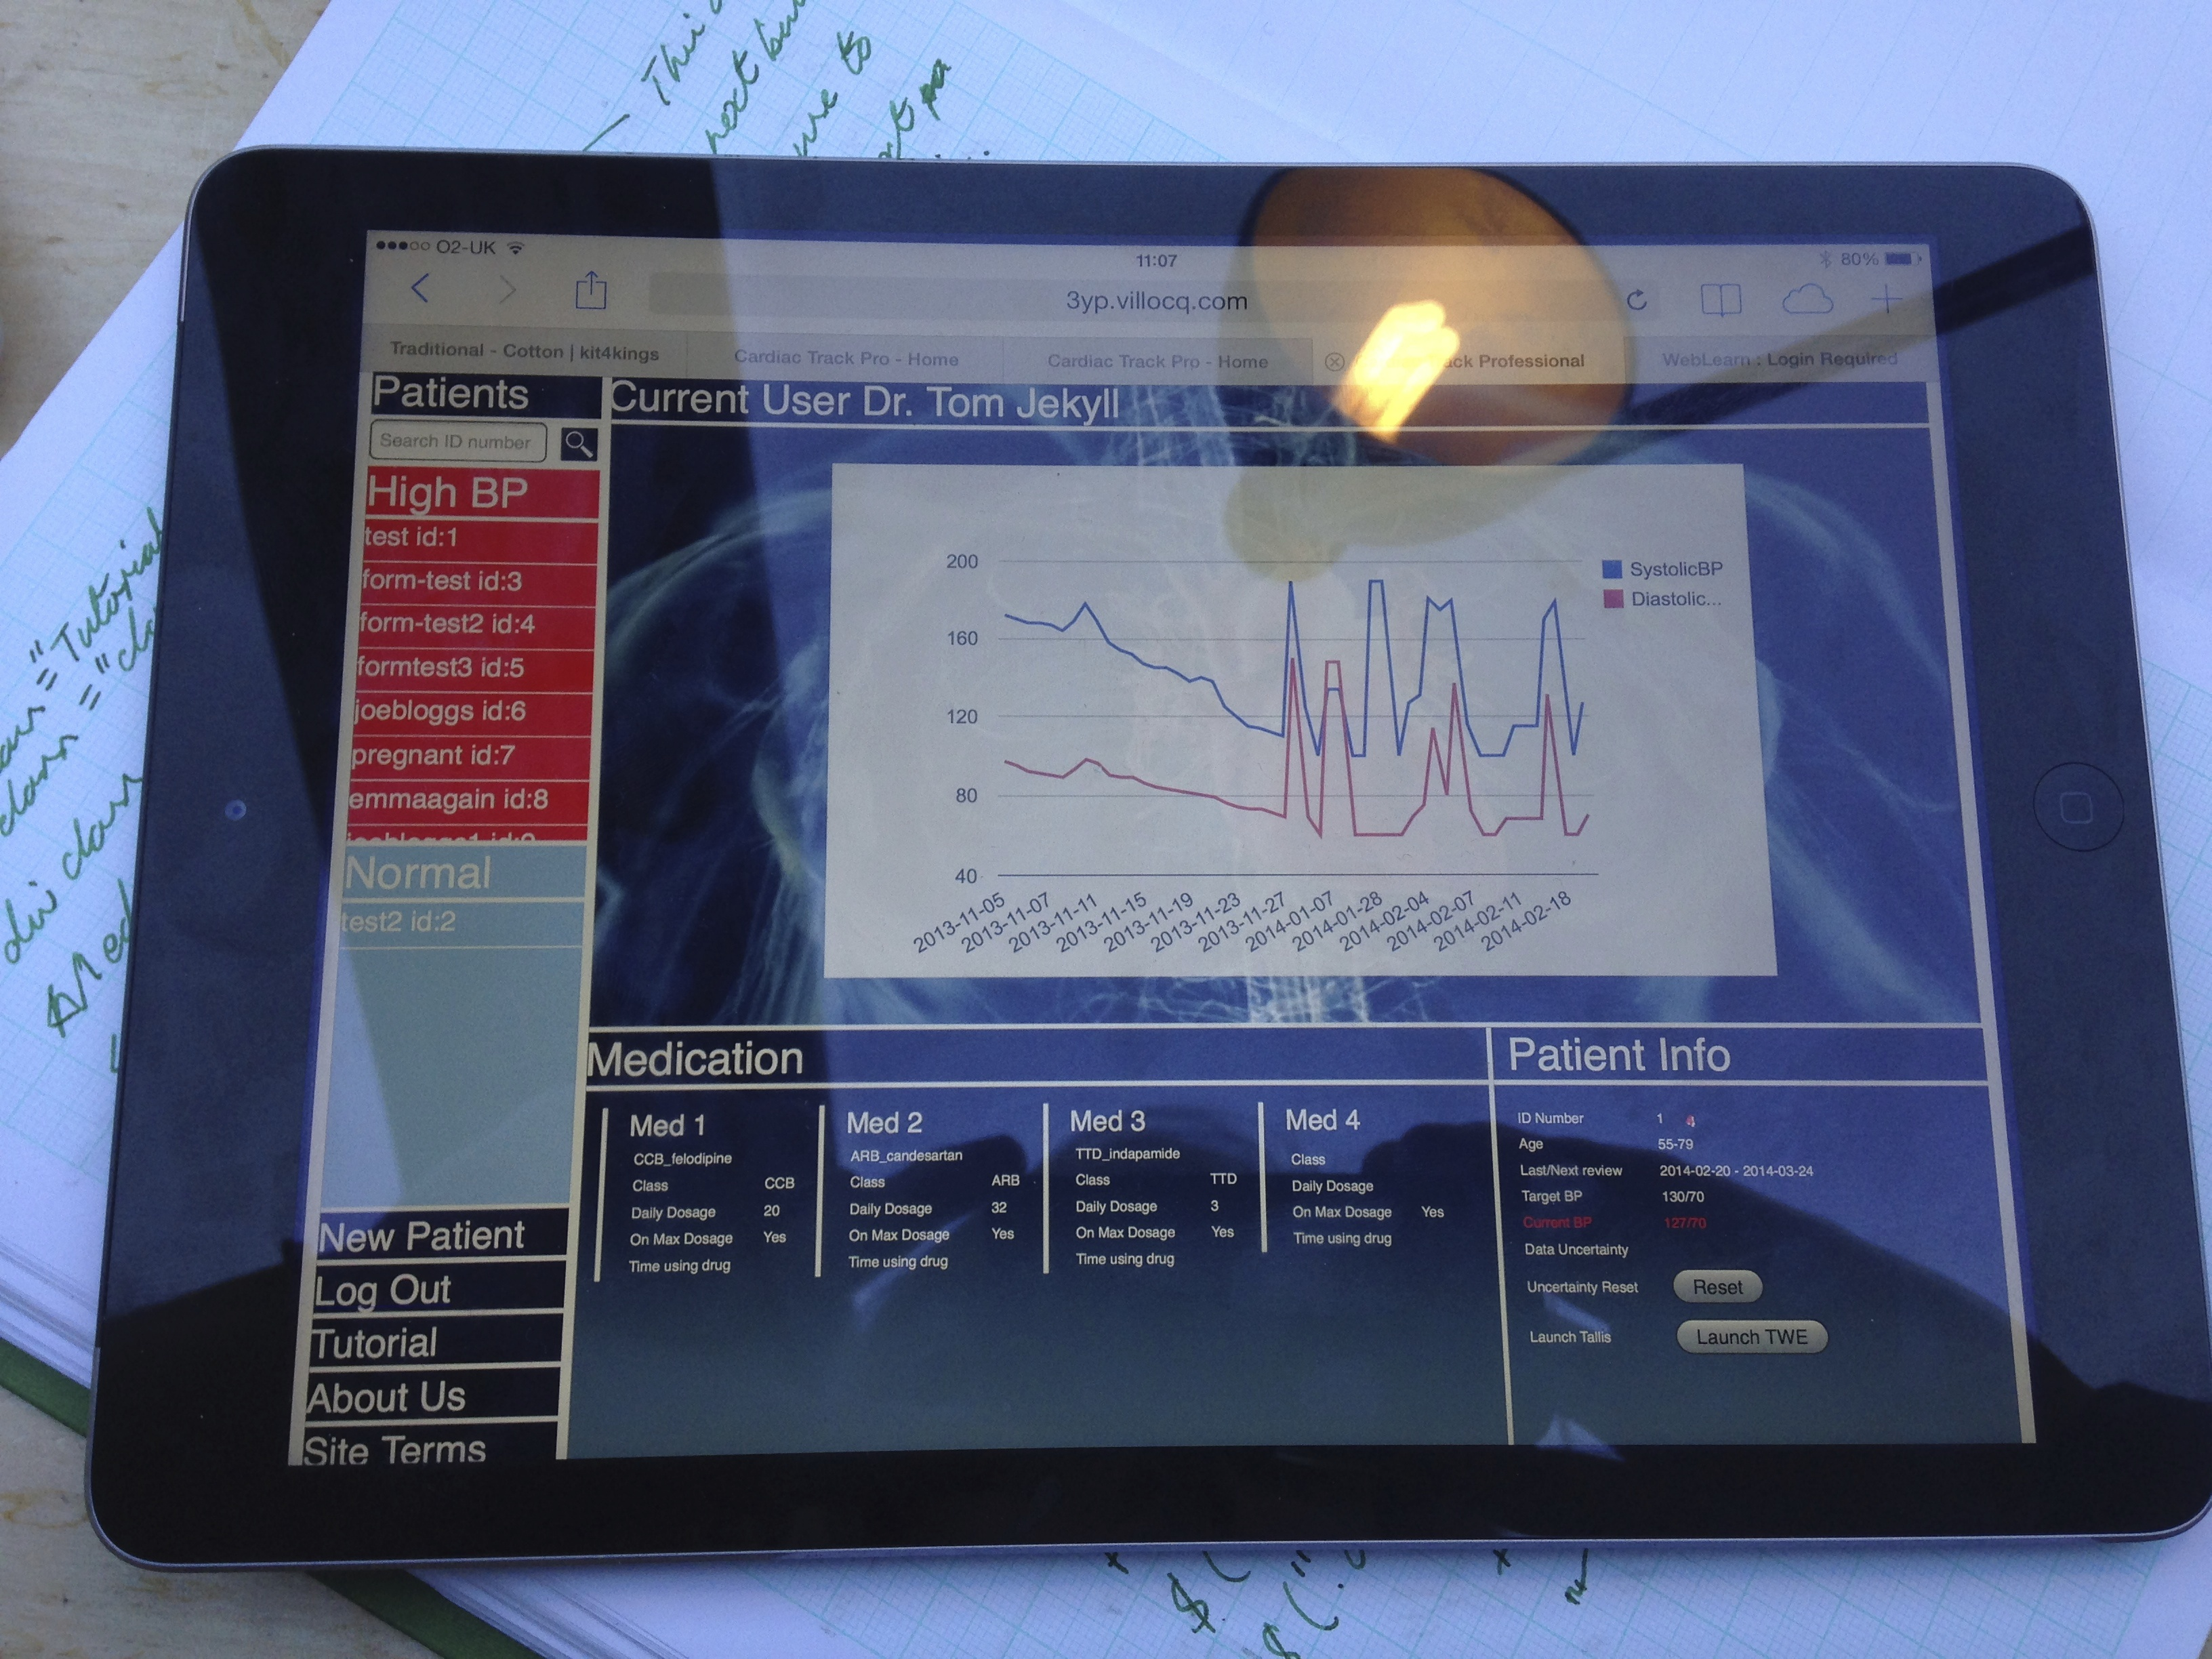
\includegraphics[scale=0.04]{ipad.png}
\caption{index.php tablet comaptibility \label{ipad}} 
\end{wrapfigure} 
This led to problems due to the page being programmed on a large high resolution screen when it was opened on a smaller device or in a smaller window the size of the div's change dramatically in terms of pixel width however the text remained constant. This caused the page to become a jumbled with text overflowing off the page. This problem was solved with the use of a new tag introduced in the 3rd version of CSS. The new units are denoted vh (for height) and vw (for width), 1 unit corresponds to $1/100$th of the viewport's height or width respectively. What makes this so useful is that it can also be used for scaling text. Therefore when the page is loaded both the font and dimensions are set in proportion to the viewport. The graph container CSS in fig.\ref{CSSscaling} to shows this, note that the original percentage settings are still kept. This is so that if someone is using an old browser that is not updated for CSS3 the divs will still be created in the old style. Using this new scaling technique means that the site is also compatible with tablet's, fig.\ref{ipad}. Also note in fig.\ref{CSSscaling}, the "background-image:url('cardioPic5.jpg')" command means that the jpg image which is saved within the currentpatients folder on the website is shown. Its repetition is set to "no-repeat" as without this the image is shown in its original pixel size but is repeated in a grid format. 

\subsubsection{Patient Selector} 
This is what the doctor uses to select the patient who he whishes' to review. Firstly the list of "High BP" and "Normal" patients seen on the left of fig.\ref{indexover} had to be dynamically created using details called from the database. This was done using PHP within the index.php page. The SQL statement in the first line of fig.\ref{selectorphp}, "SELECTS" all the patient id's "FROM" the patientInfo table whose BP is stated as being uncontrolled and who are patients of the doctor currently logged into the application. The "mysql\_num\_rows" sets the varaible\$num with the number of patients that have been selected in the SQL query and hence the number of iterations the following "while" loop needs to perform. 
\begin{figure}[h!] 
\minipage{0.59\textwidth}
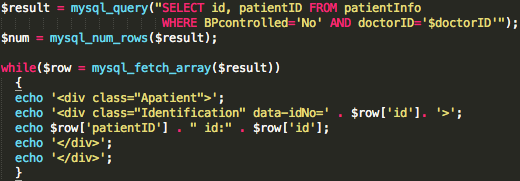
\includegraphics[width=\linewidth]{selectorphp.png}
\caption{Calling patient data from DB and dynamic div creation \label{selectorphp}}
\endminipage\hfill
\minipage{0.39\textwidth}
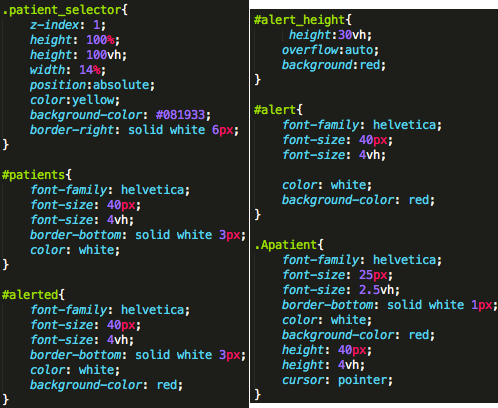
\includegraphics[width=\linewidth]{selectorCSS.png}
\caption{Patient selector CSS}
\endminipage
\end{figure} 
The "while" loop is used to write the html code which forms the div's for each individual patient. The "echo" function in PHP allows items to be written in the html script of a page, this extends to div's as well as plain text. Therefore the first line of the while function opens the div "Apatient",fig.\ref{selectorphp}. It's CSS styling sets the size, font-colour, background and border for the div. It also contains the "cursor: pointer" command this enhances usability by changing the cursor style when it is hovering over the div showing the user it is clickable. The next line of the while function creates the Identification div, this has no styling related to it but instead a data tag label idNo, "data-idNo='.\$row['id'].'$>$". This means that each div has a unique data tag which corresponds to the id number of the patient, which is called from the SQL \$row result array in PHP. This is required for selecting the patient using JavaScript. The central echo row simply writes the patient data from the same array into the div so it is displayed on the page. Note this code only forms the alerted section the normal section's code is very similar. 

\begin{wrapfigure}{l}{.34\textwidth}
\centering
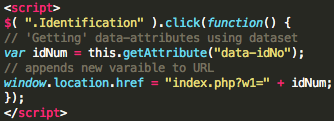
\includegraphics[scale=0.5]{selectfunc.png}
\caption{JavaScript selection function \label{selectfunc}} 
\end{wrapfigure}
The second step of implementation was the ability to bring up a patients data by clicking on their name in the list. This was done by using the JavaScript function, fig.\ref{selectfunc}. The first line within the $<$script$<$ tags (which switches the language in between them to be in JavaScript) sets the condition for initialising the function, which is on clicking an ".Identification" div. Once a function has been enacted it creates a variable "idNum" and sets this equal to the data-idNo attribute linked to that div. Finally the "window.location.href = "index.php?w1=" + idNum" function appends the newly created variable to the URL of the page creating a global variable "w1". The page reloads with this global variable in the URL, which can be accessed in PHP scripts within the page using the command "\$ \_GET["w1"]". This is the only way (bar a very similar jQuery AJAX method) in which a variable can be passed from JavaScript to PHP due to the fact the PHP runs on the server side it has no link to what happens within the JavaScript which is performed on the client side in the browser. 
\\ \indent
Patient selection was also implemented in a search bar, to enhance the usability for the doctor when dealing with large numbers of patients and the common scenario of needing to quickly find a particular patient when they come to be checked in the clinic. The search bar is found above the patient selector container on the top left of the page shown in fig.\ref{indexover}. The search bar is a html form, fig.\ref{searchbarhtml}. 

\begin{wrapfigure}{l}{0.70\textwidth}
\centering
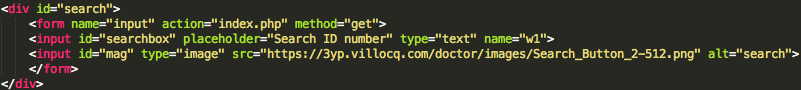
\includegraphics[scale=0.4]{searchbarhtml.png}
\caption{Html for the search bar \label{searchbarhtml}} 
\end{wrapfigure}
The form is initialised in the first line, action specifies the URL to which the forms data is directed, which in this case will be the same page. The "method="get"" command is what tells the form to append the data inputted to the URL, for this application it is the specific patient id variable. The next line sets the attributes of the search bar. The placeholder value is set so the doctor knows what they must enter and "name="w1"" is what is used to name the variable inputted. Note w1 again is used so the appended variable in the URL can be called by the PHP script in the same way. Finally the second input line screens the image of the magnifying glass which is used instead of the standard text search button to improve aesthetics. Once a patient id is entered into the bar and the magnifying glass is clicked the page is reloaded with the inputted id number appended to the URL as the global w1 variable, thus producing the patients data within the page. 

\subsubsection{Graph}
As an aid to diagnosis the variation of the patients BP over time is presented graphically to the doctor. This is done using the same Google JavaScript package as was used within the patient app, for further details on its implementation refer to the patient application UI section. The one difference from the patient app was that it was not possible to call the graph-data.php script to import the relevant data array. This is due to the fact that global page variable "w1" which denotes the user selected is required in the SQL data query. As the graph-data.php is a small script the simple solution of copying its contents into the body of JavaScript was acceptable. The SQL query was also updated to include the w1 variable so that it was updated upon a new patient being selected. 

\subsubsection{Patient information}
This section is found at the bottom of fig.\ref{indexover}. Firstly the data had to be called from the database and be formed into a series of arrays. The SQL queries for the data are shown in fig.\ref{infoSQL}, note that the "*" refers to all data being called for the relevant patient. The relevant data was then displayed in a html table by creating a short PHP section within the relevant cells which selects data from the array and displays it using echo command. Fig.\ref{medtable} shows the table for the first piece of medication, the $<$tr$>$ tags surround rows and the $<$td$>$ create cells within these rows. 

\begin{wrapfigure}{l}{0.35\textwidth}
\centering
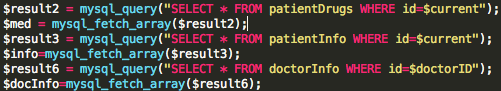
\includegraphics[width=\linewidth]{infoSQL.png}
\caption{Calling patient information from DB \label{infoSQL}}
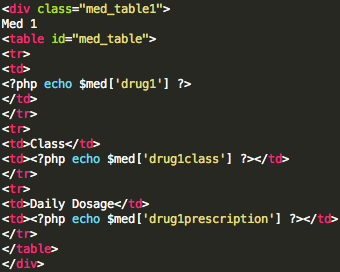
\includegraphics[width=\linewidth]{medtable.png}
\caption{Formatting patient medication data \label{medtable}}
\end{wrapfigure} 
The patient info section is similar in creation however it does include the uncertainty bar and two buttons. The uncertainty bar is formed using jQuery, therefore scripts and links had to be imported within the page header, fig.\ref{buttonscripts}. The linked scripts contain the JavaScript functions that constructs the bar. All that is required is to specify a div in which it should appear in this case "\#progressbar" and then set the value which here is the "\$flagno" (the patients data uncertainty) multiplied by 10 as the bar has 100 increments, fig.\ref{progressbar}. Outside the script in the html the div is created and given the required id="progressbar". The metric value is displayed on top of of the bar in the class="progress-label". 

\begin{figure}[h!] 
\minipage{0.49\textwidth}
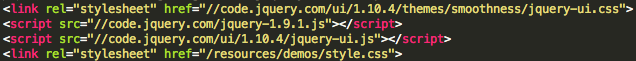
\includegraphics[width=\linewidth]{buttonscripts.png}
\caption{Calling in jQuery scripts \label{buttonscripts}}
\endminipage\hfill
\minipage{0.49\textwidth}
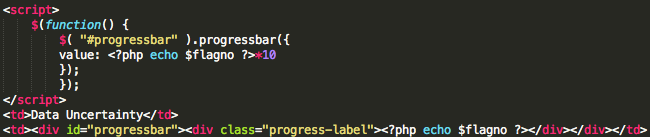
\includegraphics[width=\linewidth]{progressbar.png}
\caption{Creating the uncertainity bar \label{progressbar}}
\endminipage
\end{figure} 
The first button seen below is the uncertainty metric reset button, this calls a PHP script which enacts a single SQL query, "UPDATE patientInfo SET fraudFlag='0' WHERE patientID = '\$patientUsername'" this resets the patients uncertainty metric to 0. The second button opens the Tallis enactment script within a new window allowing the patient to be reviewed.

\subsubsection{Tutorial, About Us and Site Terms}
All of these are initiated within the bottom left hand of the index.php file. They each display their data in a similar format, with the tutorial being slightly more complex. The tutorial was included to aid usability for the doctor. Due to the time pressures GP's are under they will not have time to figure out how an application works and so may not use it unless they are succinctly taught how to operate it. The tutorial as shown from fig.\ref{tut}, highlights segments of the page individually and displays text on how to use them. The "About Us" and "Site Terms" are in the exact same format as the first tutorial section and just display the relevant data. 
\begin{figure}[h!] 
\minipage{0.49\textwidth}
\centering
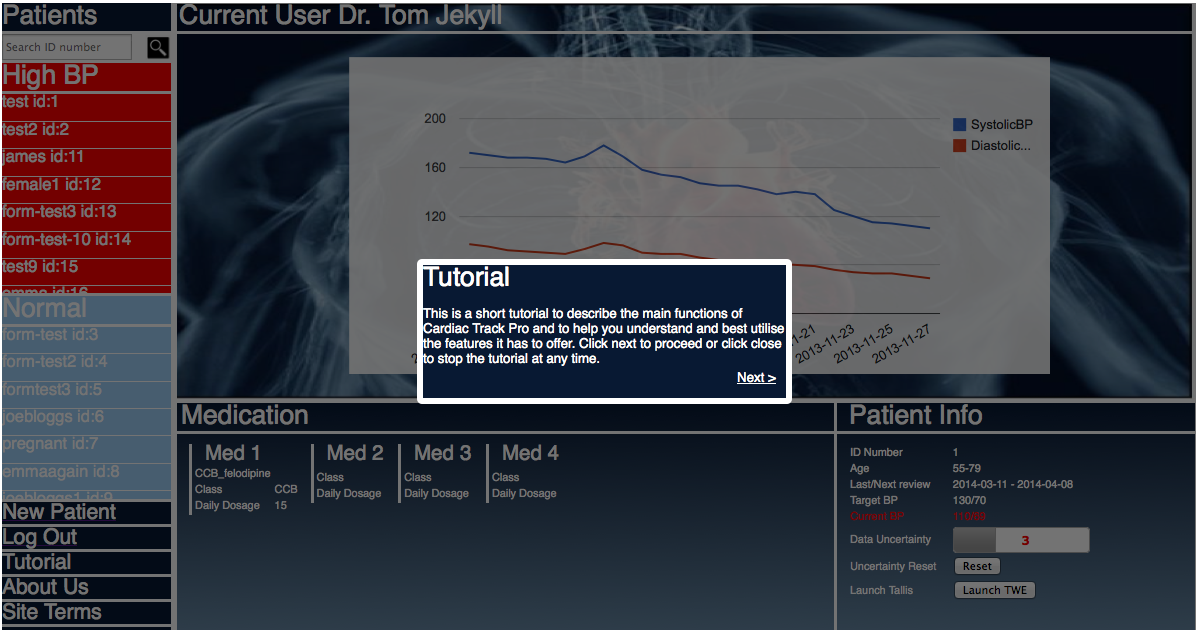
\includegraphics[width=0.8\linewidth]{tutorial1.png}
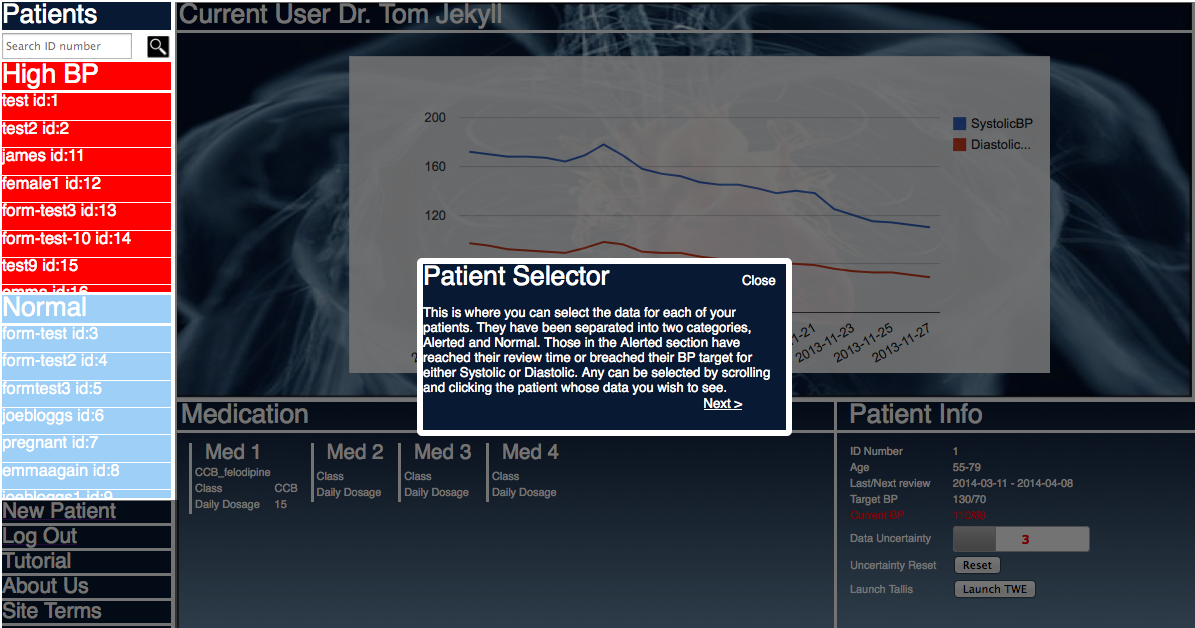
\includegraphics[width=0.8\linewidth]{tutorial2.png}
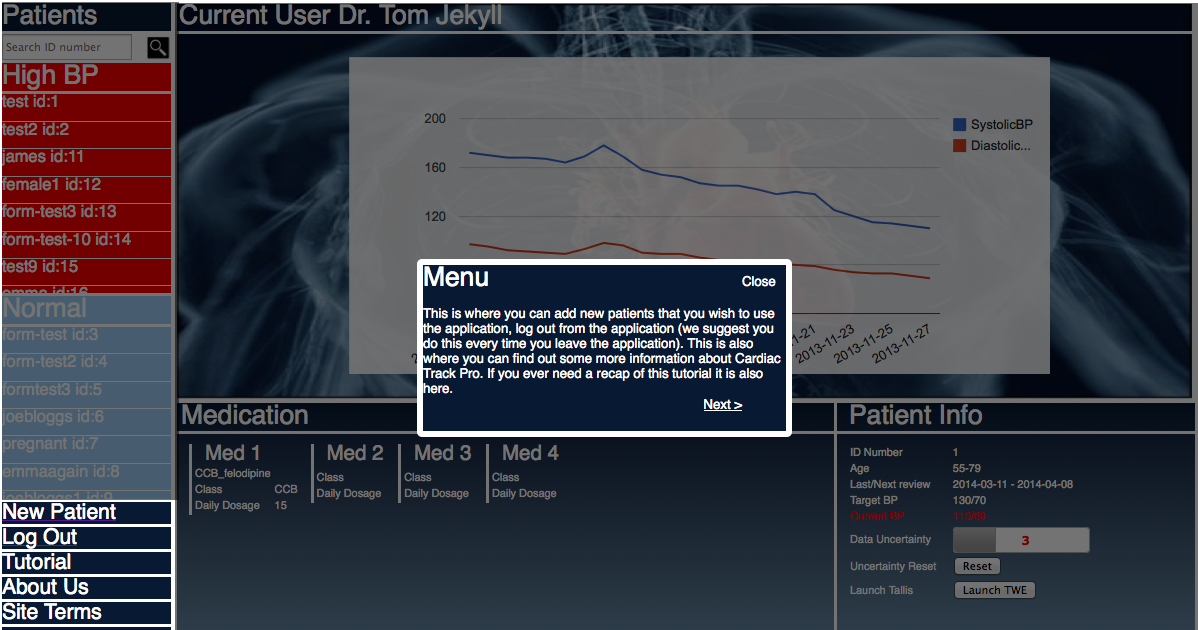
\includegraphics[width=0.8\linewidth]{tutorial3.png}
\endminipage\hfill
\minipage{0.49\textwidth}
\centering 
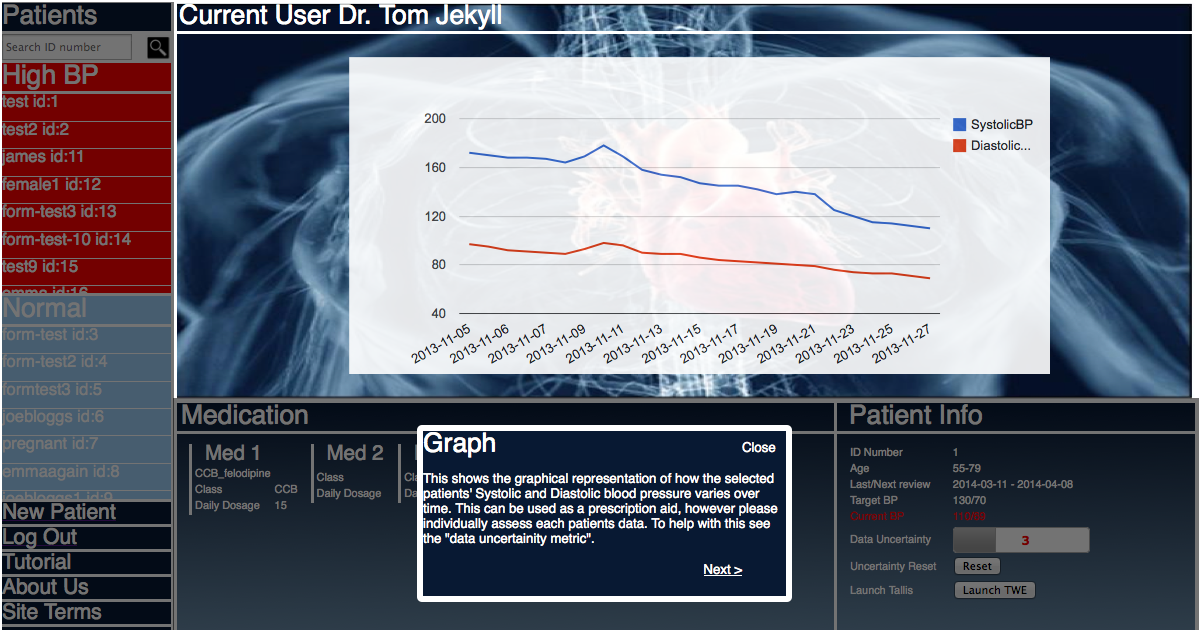
\includegraphics[width=0.8\linewidth]{tutorial4.png}
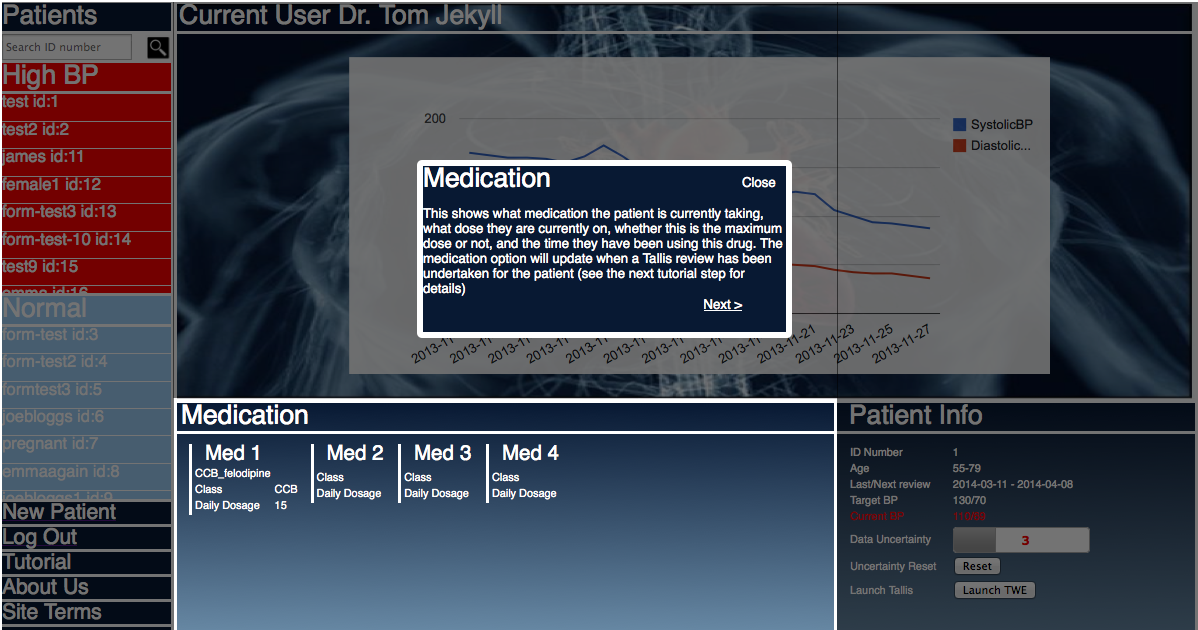
\includegraphics[width=0.8\linewidth]{tutorial5.png}
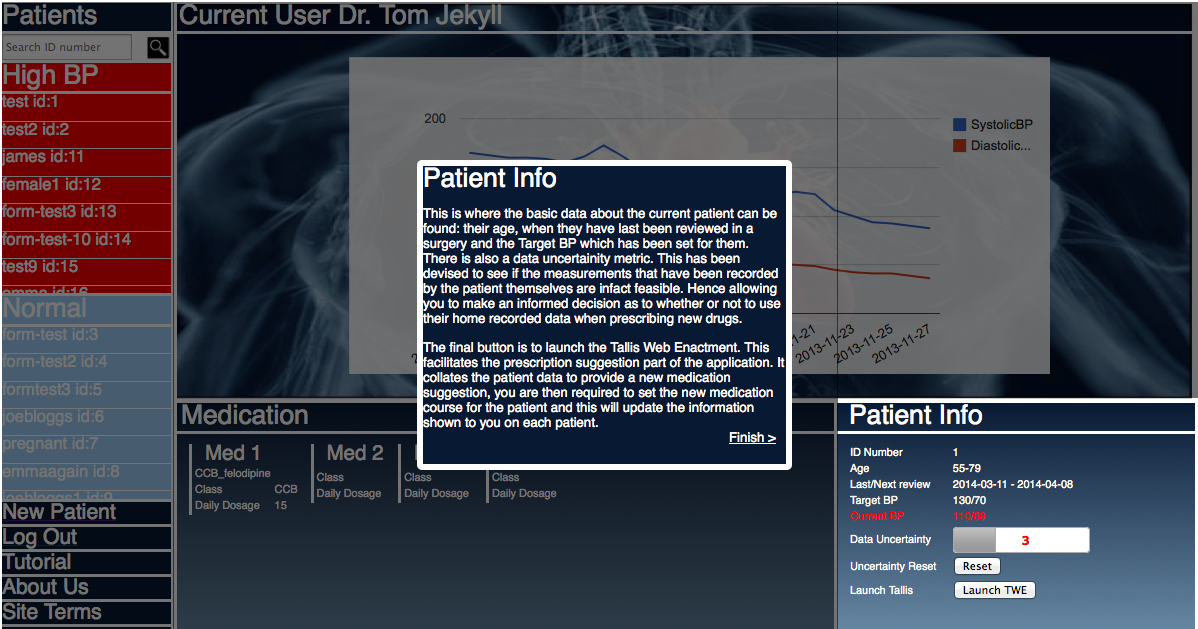
\includegraphics[width=0.8\linewidth]{tutorial6.png}
\endminipage
\caption{Tutorial \label{tut}}
\end{figure} 
The first stage of the implementation was creating the multitude of different divs that form the tutorial. The background shading is a div that covers a section of the viewport, has a black background colour and its opacity set to 55\%. In the first section of the tutorial the background can be set with a single div however the subsequent sections require multiple background divs to leave the highlighted section uncovered. The CSS command "z-index" is used to set the layering of different divs, the higher the "z-index" the further to the front the div is placed. The "z-index" of the background is set to 90 and then the text box is set to 92 so that is placed on top. The text box also has its opacity set to 1, as seen in fig.\ref{tutcss}, the "!important" is used so that this command is not overwritten.
\begin{wrapfigure}{r}{0.35\textwidth}
\centering
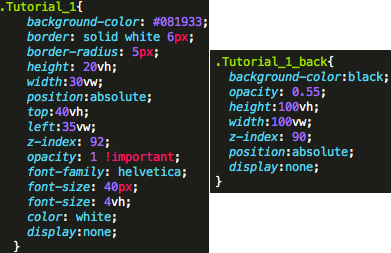
\includegraphics[scale=0.4]{tutorialCSS.png}
\caption{Tutorial section 1 CSS \label{tutcss}} 
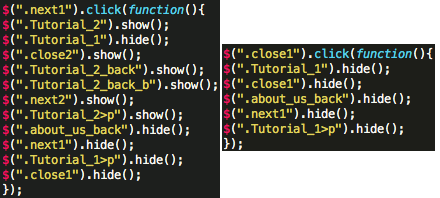
\includegraphics[scale=0.4]{tutorial1jQuery.png}
\caption{Tutorial section 1 jQuery \label{tutjq}} 
\end{wrapfigure}
All of the divs that are made to use up the tutorial have the CSS command "display:none;" meaning that when the page loads they are unseen until the jQuery function is enacted. As seen in fig.\ref{tut} all the tutorial sections bar the first and last contain a "next" and "close" button, these are the action buttons that enact the jQuery functions seen in fig.\ref{tutjq}. The top line of the function selects the relevant div which when clicked causes the commands within the \{\} brackets to take place. The jQuery functions affect the display command within the CSS, fig.\ref{tutcss}. The previous tutorial div's are hidden by the ".hide();" command which sets the CSS of the div back to "display:none;". Simultaneously the next tutorial's divs are shown with the ".show();" command. This was a very time intensive aspect of the page to implement as unique individual divs had to be made for each section of the tutorial because the jQuery function would not be able to distinguish between two divs with the same name. 

%%%%%%%%%%%%%%%%%%%%%%%%%%%%%%%%%%%%%%%%%%%%%%%%%%%%%%%%%%%%%%%%%%%%%%%%%%%%%%%%%%%%%%%%%%%%%%%%%%%%%%%%%

\section{Uncertainty Metric - \textit{Michael Fedosiuk}}

There are many reasons why testing the validity of patient inputted data is important. Patients are required to make their own blood pressure readings their accuracy will depend on the quality of the monitor used. This will depend very much on its price and is considered within the economic viability proposal. The training offered to patients using the app may not be extensive. Due to the increased prevalence of hypertension in older patients, there is a risk that many patients within this demographic may especially struggle to use the monitor to obtain accurate results. 
\\ \indent
A second type of erroneous data input may come from patients who don't take their BP readings each day. Then to fill the gaps make up readings they believe to represent accurate values.
\\ \indent
Finally patients who use the blood pressure correctly and to gain accurate readings may purposefully input fraudulent data. This is most likely to stem from a desire to limit the hypertension medication they are currently taking. Diuretics that cause less water and salt to be retained by the kidneys can cause extra urination, erection problems, weakness, fatigue and leg cramps. Beta-Blockers that cause the heart rhythm to slow and reduce ventricular force can lead to asthma symptoms, depression and insomnia \cite{webmd1}. Patients wanting to avoid drugs, which they feel may evoke such reactions, or to be removed from a drug they feel has caused such a side affect, may input lower values than they record to impact their medication.
\\ \indent
Therefore if the doctor is going to use the data as an aid to diagnosis and a possible solution for the white coat syndrome problem (see next section), it is important they are aware of the data's uncertainty. So decisions are not based on false information that may endanger the patient. Statistical methods were therefore sought to highlight data that is not deemed to be realistic. 

\subsection{Data Sourcing}

To create a statistical model a set of data is required. Due to the time and funding for this project it was not possible to test for this. It was therefore necessary to source medical journals for trials which utilised daily blood pressure (BP) measuring. In the Journal of Human Hypertension an article was found, "Detecting white coat and reverse white coat effects in clinical settings using measures of blood pressure habituation in the clinic and patient self-monitoring of blood pressure" \cite{study} .This study was conducted by the Department of Psychology at the University of West Virginia to determine how home blood pressure monitoring could be used to detect white coat syndrome. White coat syndrome is when the blood pressure of a patient when measured in a clinical setting gives a larger value than an ambulatory reading (taken at multiple points at home over 24 hours) due to the patient feeling increased stress. Similarly a patient may experience reverse white coat syndrome, which is when their blood pressure drops in a clinical setting. 
\\ \indent
The West Viginian study involved the evaluation of 54 patients for which 52 gave complete data sets. The trial took place over one week. There were 4 blood pressure measurements taken in the clinic, a single 24-hour period of ambulatory monitoring and most importantly for this project daily measurements by the patients themselves at home. The home measurements allow us to assess the normal levels of blood pressure variation. On contacting the correspondence for the paper Dr K T Larkin, the full set of data for the 54 patients was sent. 

\subsection{Metric Overview}

% Define block styles
\tikzstyle{decision} = [diamond, draw, fill=blue!20, 
text width=4.5em, text badly centered, node distance=3cm, inner sep=0pt]
\tikzstyle{block} = [rectangle, draw, fill=blue!20, 
text width=5em, text centered, rounded corners, minimum height=4em]
\tikzstyle{line} = [draw, -latex']
\tikzstyle{cloud} = [draw, ellipse,fill=red!20, node distance=3cm,
minimum height=2em]

\begin{center}
\begin{tikzpicture}[node distance = 6cm, auto]
% Place nodes
\node [cloud] (init) {Data called in from SQL DB};
\node [block, left of=init] (expert) {Linear regression test};
\node [block, right of=init] (system) {Correlation coefficient test};
\node [decision, below of=expert] (identify) {Is \% error greater than 10\%};
\node [decision, below of=system] (evaluate) {Coeff $0.98<r<-0.98$};
\node [block, right of =identify] (plus) {Uncertainty metric +1};
\node [block, below of =init] (normal) {Uncertainty metric unchanged}; 

% Draw edges
\path [line] (init) -- (expert);
\path [line] (init) -- (system); 
\path [line] (expert) -- (identify);
\path [line] (system) -- (evaluate);
\path [line] (identify) -- node [near start] {yes} (plus);
\path [line] (evaluate) -| node [near start] {yes} (plus); 
\path [line] (identify) |- node [near start] {no} (normal);
\path [line] (evaluate) |- node [near start] {no} (normal); 
%\path [line] (update) |- (identify);
%\path [line] (decide) -- node {no}(stop);
%\path [line,dashed] (expert) -- (init);
%\path [line,dashed] (system) -- (init);
%\path [line,dashed] (system) |- (evaluate);
\end{tikzpicture}
\end{center}

\subsection{Metric make up} 
 A number of assumptions about the nature of the data were required so this data set could be used: 
\begin{enumerate}
\item 
The data was collected from patients that were not taking any anti-hypertension medication, which could affect their blood pressure or heart rate. The assumption is made that over the course of one week the patients heart rate should be constant to the extent that it can be modelled linearly, with a realistic level of variance. We then must assume it is comparable to the patients who are using our app after the month period when any affect from new medication has stabilised. 
\item 
The patients in the test have not lied. It is a medical trial and hence will not impact the medication of the patients removing any reason to lie.
\item 
The training and the blood pressure monitors received by the patients in the trial would be comparable to that given to people who will use the app. If either quality is reduced it will mean that the data collected by patients using the app may have an increased variance compared to the trial data.
\item
The variance of blood pressure over time for patients taking anti-hypertension medication is the same as those who are not taking anti-hypertension medication. Which is required if we are to use this data set as a representation of medicated patient data.
\end{enumerate}

Although there are risks which come with these assumptions, accepting them meant that we were able to implement a linear model for the set of seven daily blood pressure measurements of each patient. The analysis was initially performed in Excel, this was chosen because it was readily available, the data was already in this format and it allowed for simple data manipulation and graphical representation.

\subsubsection{Linear Regression}
Linear regression is a set of mathematical operations that creates a line of best fit for a set of scattered data points. Linear regression can either be multivariate linear regression or simple linear regression. Multivariate analysis allows you to considered multiple variables whereas simple regression analysis just relates a single driven variable. 

\begin{wrapfigure}{r}{.40\textwidth}
\centering
\fbox{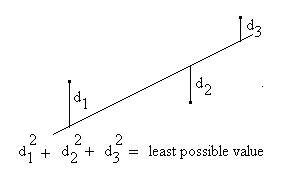
\includegraphics[scale=0.4]{linexmp.png}}
\caption{Least Squares Linear Regression Overview \cite{linregdia} \label{linregfig}}
\end{wrapfigure} 
For this application simple regression analysis was sufficient, to asses the single variable of BP over time. The use of linear regression usually falls within two main segments, prediction and correlation. This use of the model falls within the correlation category. For correlation testing a given variable $Y$ , in this model BP measurements relates a number of driving variables $X_1, X_2,...,X_i$ , in this model time progression. These are analysed with a linear regression to find out how strongly they are related and to highlight which values of $X_1, X_2,...,X_i$ contain data which does not conform.
\\ \indent 
In this model, linear least squares regression is "The straight line $y=a + bx$ should be fitted through the given points $(x_1,y_1)...(x_i,y_i)$ so that the sum of the squares of the distances of those points from the straight line is minimum, where the distance is measured on the vertical direction (the y-direction)" \cite{Kryzig}. Each data point is of the form shown below:
\begin{figure}[h]
\minipage{0.50\textwidth} 
\begin{equation}
Y_i=m_0 +m_1X_i +r_i
\end{equation} 
\endminipage\hfill
\minipage{0.40\textwidth}%
$Y_i=$BP data value
\\$X_i=$Day's corresponding number
\\$m_0=$regression const. sets $Y$ intercept
\\$m_1=$regression coeff. sets effect of $X$
\\$r_i=$residual; error between line and data
\endminipage
\end{figure}

\begin{wrapfigure}{r}{.28\textwidth}
\begin{equation}
S=\sum\limits_{i=1}^N r_i^2
\end{equation}
\begin{equation}
S=\sum\limits_{i=1}^N (Y_i-m_0 -m_1X_i)^2
\end{equation}
\end{wrapfigure} 
\noindent The derivation, based on \cite{linregdev}, starts with the sum of the squared residual values mathematically represented as shown in eq.2. This is the value that must be minimised with respect to the values of $m_0$ and $m_1$ therefore we need to express the value of $S$ in terms of $m_0$ and $m_1$, eq.1, eq.2 and eq.3. This now means that partial derivatives can be used to minimise the equation in terms of both $m$ values, these derivatives are shown below with $m_0$ on the left and $m_0$ on the right.

\begin{figure}[h]
\minipage{0.50\textwidth} 
\begin{equation}
\frac{\partial S}{\partial m_0} = \sum\limits_{i=1}^N \Big[ \frac{\partial }{\partial m_0} (Y_i-m_0 -m_1X_i)^2 \Big]
\end{equation} 
\begin{equation}
\frac{\partial S}{\partial m_0} = -2\sum\limits_{i=1}^N (Y_i-m_0 -m_1X_i)^2 
\end{equation} 
\endminipage\hfill
\minipage{0.50\textwidth}%
\begin{equation}
\frac{\partial S}{\partial m_1} = \sum\limits_{i=1}^N \Big[ \frac{\partial }{\partial m_1} (Y_i-m_0 -m_1X_i)^2 \Big]
\end{equation}
\begin{equation}
\frac{\partial S}{\partial m_1} = -2\sum\limits_{i=1}^N X_i(Y_i-m_0 -m_1X_i)^2 
\end{equation}
\endminipage
\end{figure}
The minimum is required so both derivatives need to be set equal to 0, let us first consider the $m_0$ derivative. Algebraic manipulation is used to separate the $m$ coefficients and then it is divided by $-2$ see eq.5 and eq.7, so $m_0$ can be found. Eq.10 firstly shows that $m_0$ and $m_1$ have been brought outside the summation term since it is the same for all values. Finally diving through by $N$ provides the value for $m_0$ in terms of $m_1$ as a function of the mean of $X$ and $Y$.

\begin{figure}[h]
\minipage{0.35\textwidth} 
\begin{equation}
\sum\limits_{i=1}^N m_0 = \sum\limits_{i=1}^N Y_i - \sum\limits_{i=1}^N m_1X_i
\end{equation}
\begin{equation}
N m_0 = \sum\limits_{i=1}^N Y_i - m_1\sum\limits_{i=1}^N X_i
\end{equation}
\begin{equation}
m_0 = \Bigg(\frac{\sum\limits_{i=1}^N Y_i}{N}\Bigg) - m_1\Bigg(\frac{\sum\limits_{i=1}^N X_i}{N}\Bigg)
\end{equation}
\endminipage\hfill
\minipage{0.65\textwidth}%
\begin{equation}
0 = \sum\limits_{i=1}^N Y_iX_i - \sum\limits_{i=1}^N m_0X_i - \sum\limits_{i=1}^N m_1X_i^2
\end{equation}
\begin{equation}
m_1\sum\limits_{i=1}^N X_i^2 = \sum\limits_{i=1}^N Y_iX_i - m_0\sum\limits_{i=1}^N X_i 
\end{equation}
\begin{equation}
m_1\sum\limits_{i=1}^N X_i^2 = \sum\limits_{i=1}^N Y_iX_i - \Bigg[\Bigg(\frac{\sum\limits_{i=1}^N Y_i}{N}\Bigg) - m_1\Bigg(\frac{\sum\limits_{i=1}^N X_i}{N}\Bigg)\Bigg] \sum\limits_{i=1}^N X_i 
\end{equation}
\endminipage
\end{figure} 

The next step is to find $m_1$, this is done using the partial derivative with respect to $m_1$, eq.6 and is similarly set equal to 0 so the minimum point can be found. Rearranging and removing the $-2$ transforms eq.7 into eq.11. 


\begin{wrapfigure}{r}{.60\textwidth}
\begin{equation}
m_1\sum\limits_{i=1}^N X_i^2 = \sum\limits_{i=1}^N Y_iX_i - \frac{\sum\limits_{i=1}^N Y_i \sum\limits_{i=1}^NX_i}{N} - m_1\Bigg[\frac{\bigg(\sum\limits_{i=1}^NX_i\bigg)^2}{N}\Bigg]
\end{equation}
\begin{equation}
m_1 = \frac{\sum\limits_{i=1}^N Y_iX_i - \frac{\sum\limits_{i=1}^N Y_i \sum\limits_{i=1}^NX_i}{N}} {\sum\limits_{i=1}^NX_i^2-\frac{\bigg(\sum\limits_{i=1}^NX_i\bigg)^2}{N}}
\end{equation}
\end{wrapfigure} 
Once again the next step is to move the $m$ constants outside of the summation. Then to solve for $m_1$ we need to eliminate $m_0$ which is done through the substitution of eq.10, giving eq.13. Subsequently $m_1$ can be found in terms of $X_i$, $Y_i$ and $N$, eq.14 to eq.15. Once eq.15 and 10 have been implemented to find the $m_0$ and $m_1$ coefficients it is then possible to combine them in eq.1 to find the least squares linear regression. 
\\ \indent 
To reliably use the least square's regression line created, there a number of provisos which both the driving and driven variable's as well as their interaction's must satisfy. 
\begin{itemize}
\item 
\textbf{Homoscedasticity:} This requires the variance to be constant both over time and variation in the predictor values (the BP values). In our application we would expect the variance over time to remain the same for a healthy patient who has a stable BP. This is obviously dependant on the monitor they are using and that their ability to take accurate readings remains the same, and they are not imputing false data. A breach in homoscedasticity is what alerts the doctor in the form of the uncertainty metric. A potential common limitation is that variance usually increases proportionally to the size of measurement that is being taken, however this is assumed to be negligable in this application. The monitor will have a set percentage error, for example +/- 2\%, when recording a BP of 160mmHg there is +/-3.2mmHg variance however when recording a BP of 100mmHg the variance will drop to +/-2mmHg. 
\item 
\textbf{Independence:} This requires that there are no systematic errors. In this case we are using the linear regression to detect errors, which means this creates a limitation in our model. It means that if a person is systematically measuring false readings from their BP monitor the error will be missed, as the whole regression line will be shifted in the direction of the false data inputted. These systematic errors can be minimised through the quality of the BP monitor used and the training given to the patient, however both of these raise the cost of the treatment method. It does however mean that it will not be possible to catch people who cheat "realistically", i.e. slowly reducing their BP within the accepted bounds using a system based solely upon Linear Regression. 
\item 
\textbf{Normality:} This requires that the errors be normally distributed, for a normal patient who is accurately recording their BP on a fully functioning monitor this should hold true. (calculate the standard deviation) 
\end{itemize}

It was then necessary to assess the variance in the data provided by Dr Larkin to set bounds for the percentage error limitations. As previously stated eq.10 and 15 were implemented in Excel. This meant that the values of $m_0$ and $m_1$ could be found for each of the patients 7 data points. 

\begin{wrapfigure}{r}{.60\textwidth}
\centering
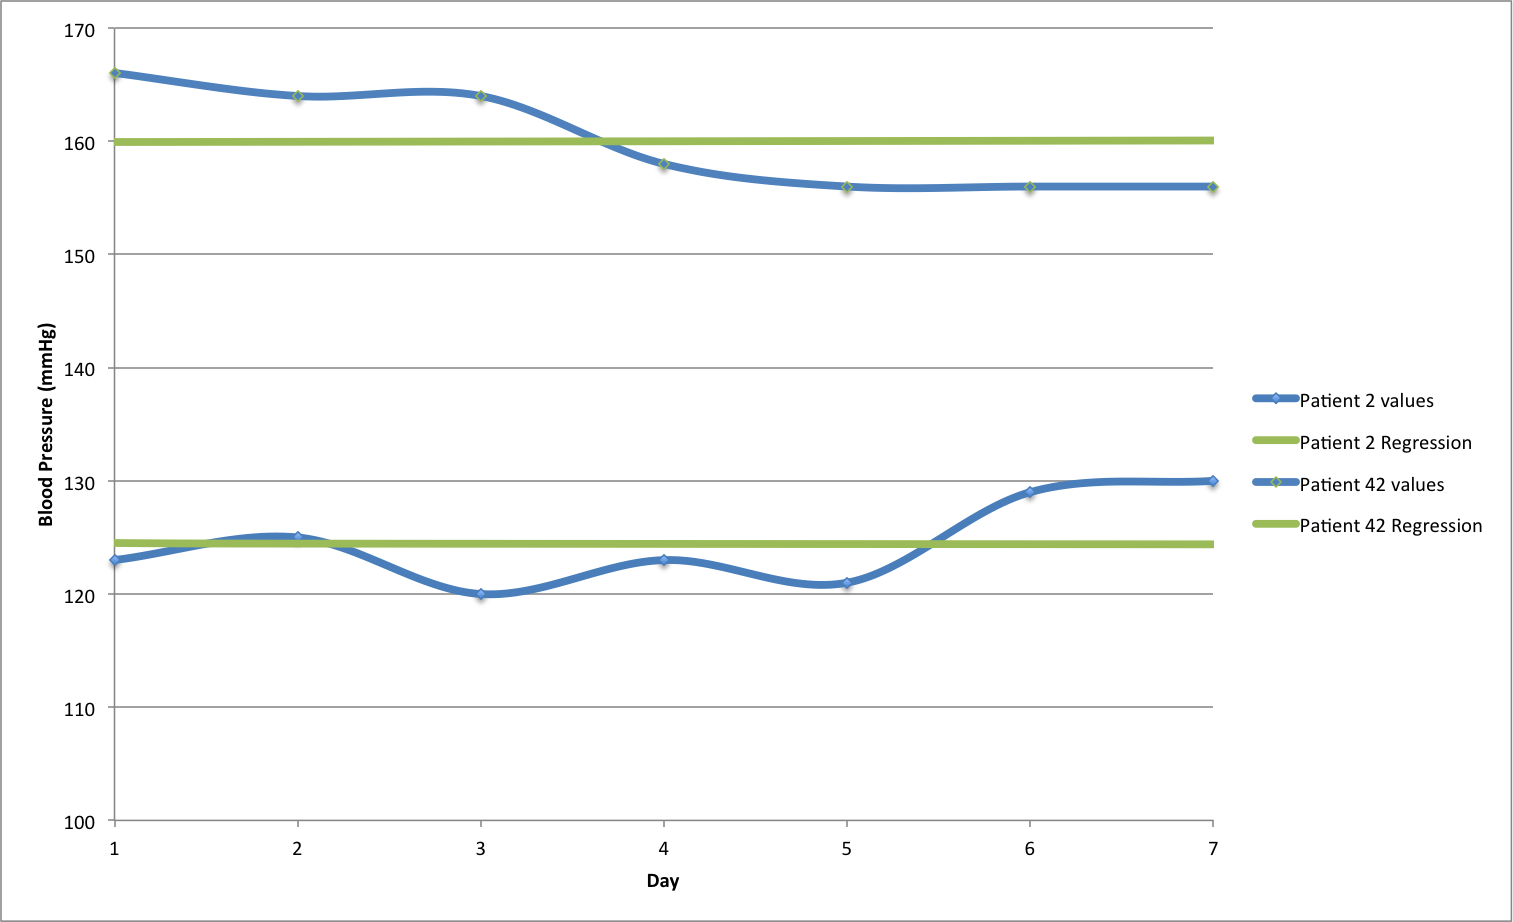
\includegraphics[scale=0.4]{replinreg.png}
\caption{Graph showing variation of BP over 7 days and corresponding linear least squares regression \label{replinreg}} 
\end{wrapfigure} 

Inputting these values into eq.1 meant that the point predicted by the Linear Regression was calculated for each of the 7 days. It was then possible to plot both the recorded data and the corresponding regression line on the same graph, fig.\ref{replinreg}. This allowed an expectable limitation on the percentage error to be found. In excel the function, =ABS(([@Day1]-[@reg1])/[@Day1]), (note that Day1 is the data the patient inputted and reg1 was the corresponding linear regression prediction) was implemented for each of the 7 days and gave the absolute value of the percentage error. Then utilising the max function in Excel, =MAX(Table1[@[Error 1 from lin]:[Error 7 from lin7]]), it was possible to find the maximum percentage error for each patient. Throughout all the 52 patients only one had a point with a percentage error greater than 10\%, at 10.10592\%. It was deemed the cut-off point for data reliability should be 10\% regarding the 10.1\% result to be an outlier (look to add in wrong outlier). Hence the uncertainty metric is increased by a single increment for each point inputted that has a greater than 10\% errors compared to the regression line in the last 7 data entries. An example is shown below, the data on the left is seen as reliable as it does not breach either the upper or lower bounds and hence has an uncertainty metric of 0. Conversely the data on the right breaches both so has an uncertainty metric of 2. 
\begin{figure}[h!] 
\minipage{0.49\textwidth}
\fbox{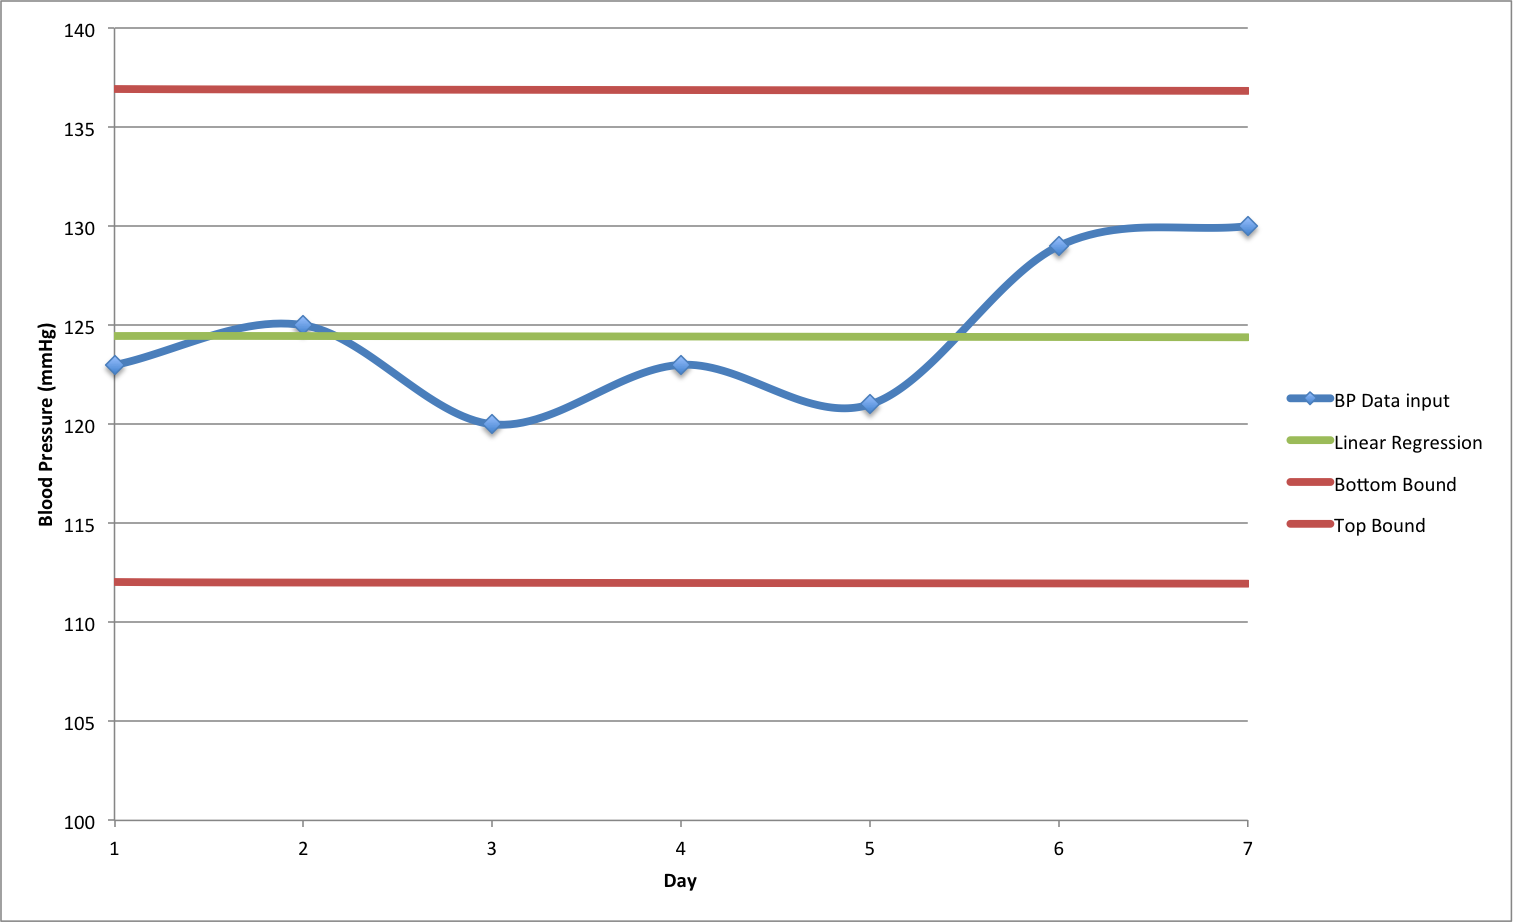
\includegraphics[width=\linewidth]{linreggood.png}}
\caption{Data with an uncertainity metric value of 0}
\endminipage\hfill
\minipage{0.49\textwidth}
\fbox{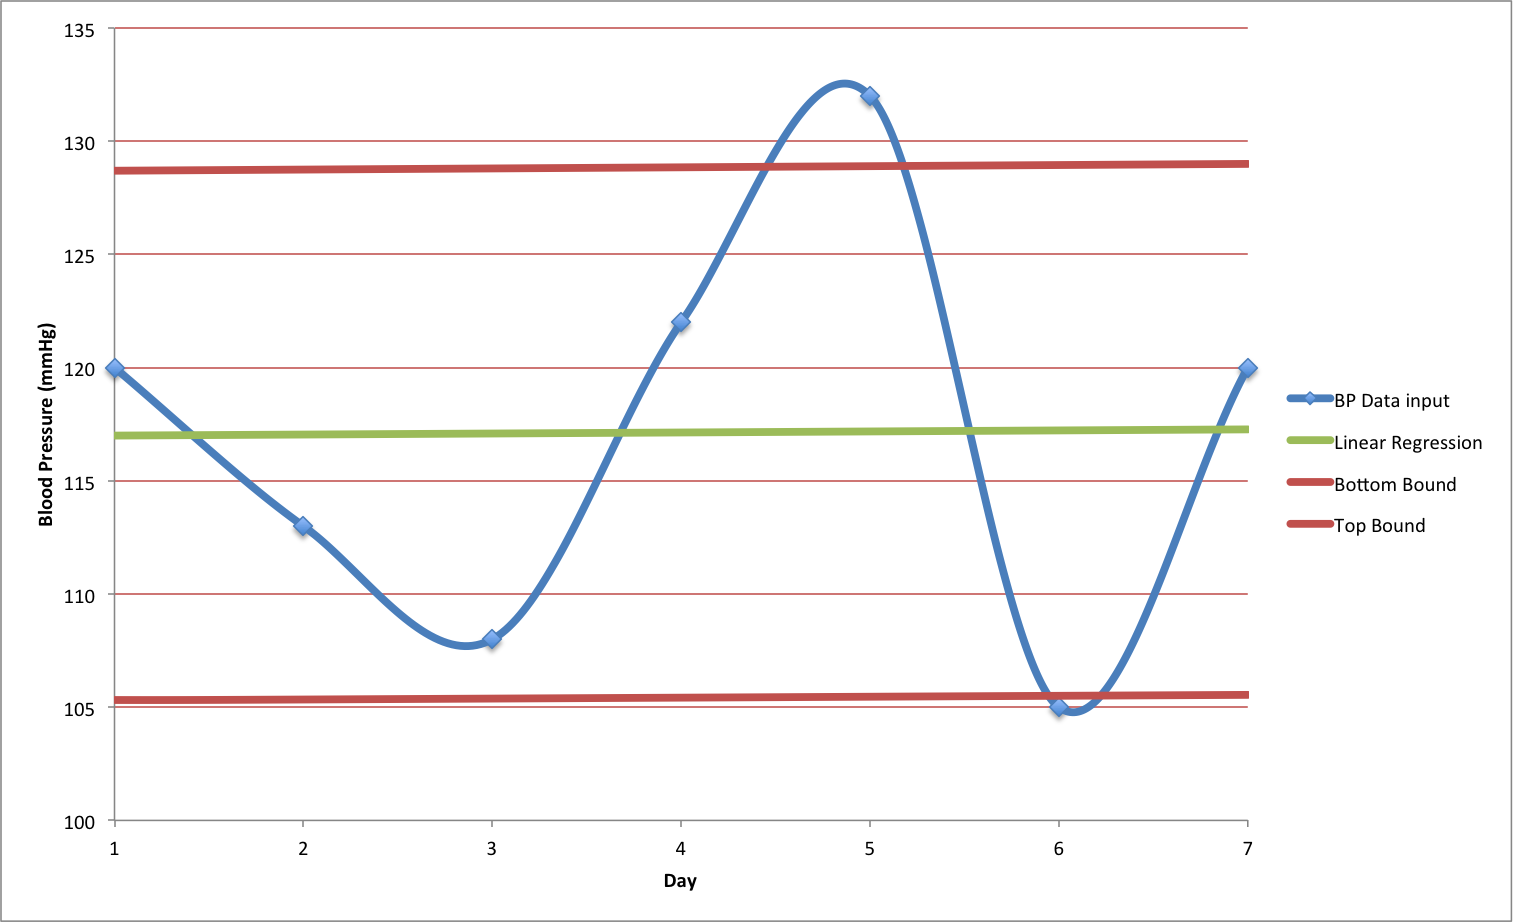
\includegraphics[width=\linewidth]{linregbad.png}}
\caption{Data with an uncertainity metric value of 2}
\endminipage
\end{figure} 

\subsubsection{Pearson product-moment correlation coefficient}
One of the limitations that was present in using the linear regression on its own was its susceptibility to systematic cheating. Due to the natural fluctuation of data each day a perfectly linear set of results would be considered false. Hence it is a sign of greater uncertainty because it is likely that the patient is falsifying measurements if this happens recurrently. This is tested for using the correlation coefficient, which finds the linear dependency between two variables. 
\\ \indent
This means that straight positive correlations yield a value of 1 and straight negative correlations yield a value of -1. If there is no correlation, i.e. a random scatter of points, a correlation of approximately 0 will be found, fig.\ref{correx}. Precise horizontal lines will also yield a correlation 0, because although it is linear the driven component is not affected by the driving component. 

\begin{figure}
\centering 
\fbox{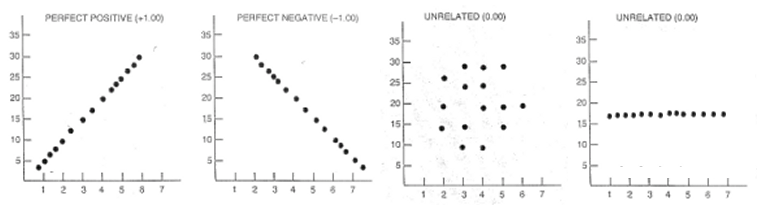
\includegraphics[width=0.7\linewidth]{correx.png}}
\caption{The coefficients given to various data sets \cite{linregex} \label{correx}}
\end{figure}

The Pearson product-moment correlation coefficient, as shown in eq.16, is the ratio of covariance of the two variables and the product of their respective standard deviations. This however must be adapted for use with a sample to use estimates of the covariance and standard deviations, giving the Pearson sample correlation coefficient, eq.17, denoted r. It can be manipulated into eq.18, which can be easily calculated using values found in the least square's regression calculations.

\begin{figure}[h!] 
\minipage{0.49\textwidth}
\begin{equation}
\rho_{X,Y} = \frac{cov(X,Y)}{\sigma_X\sigma_Y}
\end{equation}
\endminipage\hfill
\minipage{0.49\textwidth}
\begin{equation}
r = \frac{\sum\limits_{i=1}^N (X_i - \overline{X})(Y_i - \overline{Y})}{\sqrt{(X_i - \overline{X})^2}\sqrt{(Y_i - \overline{Y})^2}}
\end{equation}
\begin{equation}
r = \frac{\big(\Sigma xy - N\overline{x}\overline{y}\big)^2}{\big(\Sigma xx - N\overline{x}\overline{y}\big)\big(\Sigma yy - N\overline{x} \overline{y}\big)}
%http://en.wikipedia.org/wiki/Pearson_product-moment_correlation_coefficient
\end{equation}
\endminipage
\end{figure} x

As with the linear regression the correlation coefficient was first calculated using the test data within Excel, using the following formula $=(((7)*([@Column7]))-(([@Day8])*([@Day9])))/((((7)*([@Column15])-([@Day9]^2))^(0.5))*(((7)*([@Column158])-(([@Day8])^2))^(0.5)))$ for eq.18. Then in juxtaposition to the linear regression analysis the lowest level of variance and hence highest absolute value of the correlation coefficient was found, so that people trying to cheat methodically would be caught. The limit was set $0.98<r<-0.98$ this was significantly higher than the greatest correlation of the data. An example is shown below, the graph on the left has a correlation coefficient of -0.653 and hence the uncertainty metric remains unchanged. The graph on the right however has a correlation coefficient of -0.985 and hence breaches the limit and raises the uncertainty metric by 1. 

\begin{figure}[h!] 
\minipage{0.49\textwidth}
\fbox{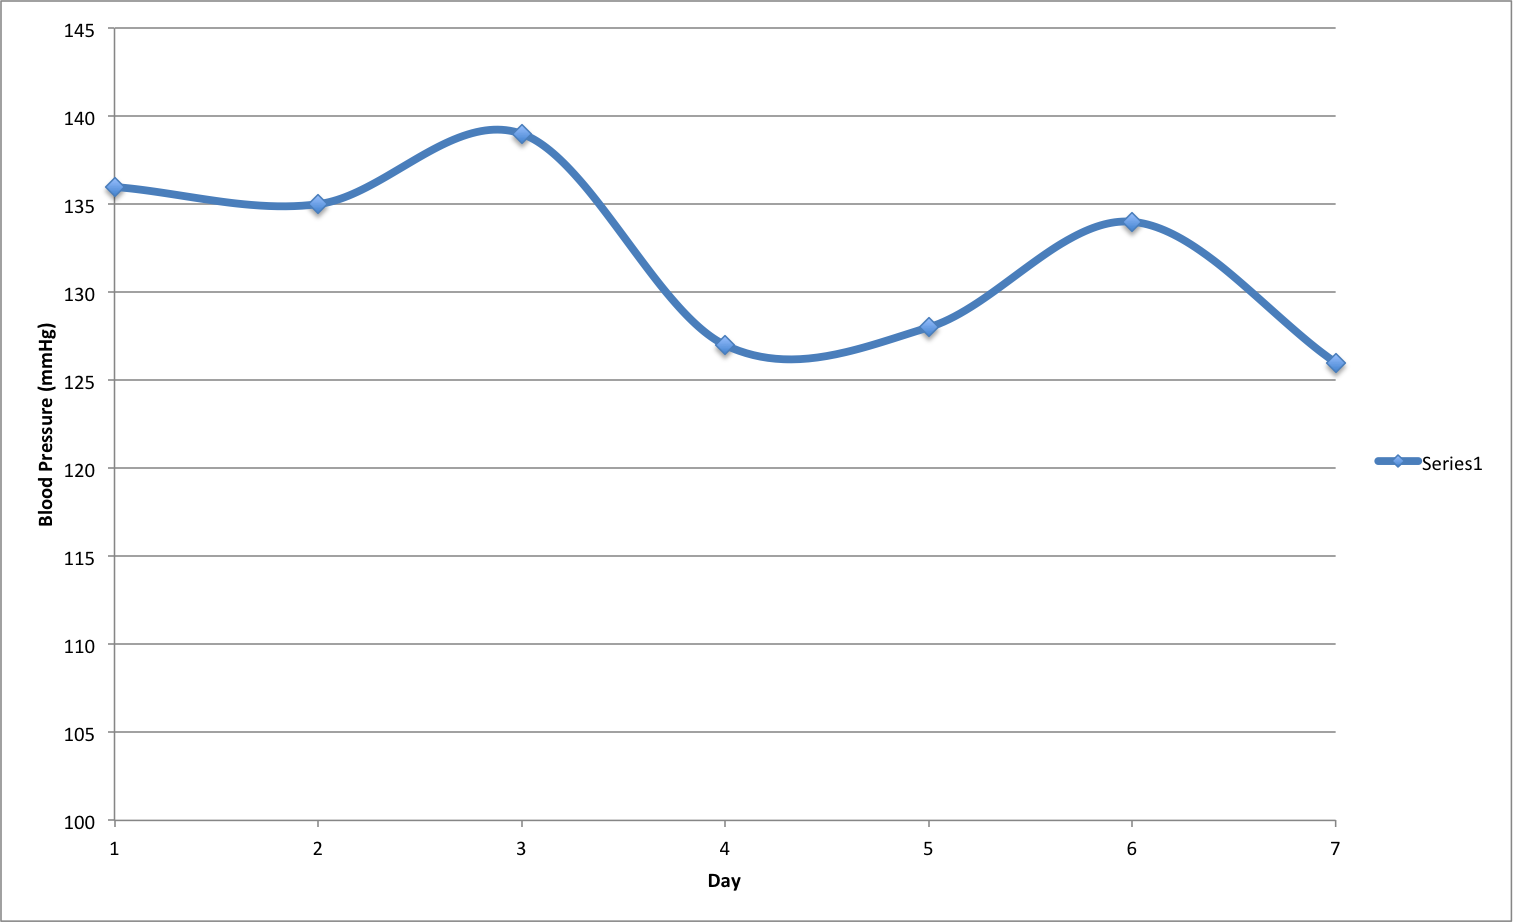
\includegraphics[width=\linewidth]{corrgood.png}}
\caption{Data with an uncertainity metric value of 0}
\endminipage\hfill
\minipage{0.49\textwidth}
\fbox{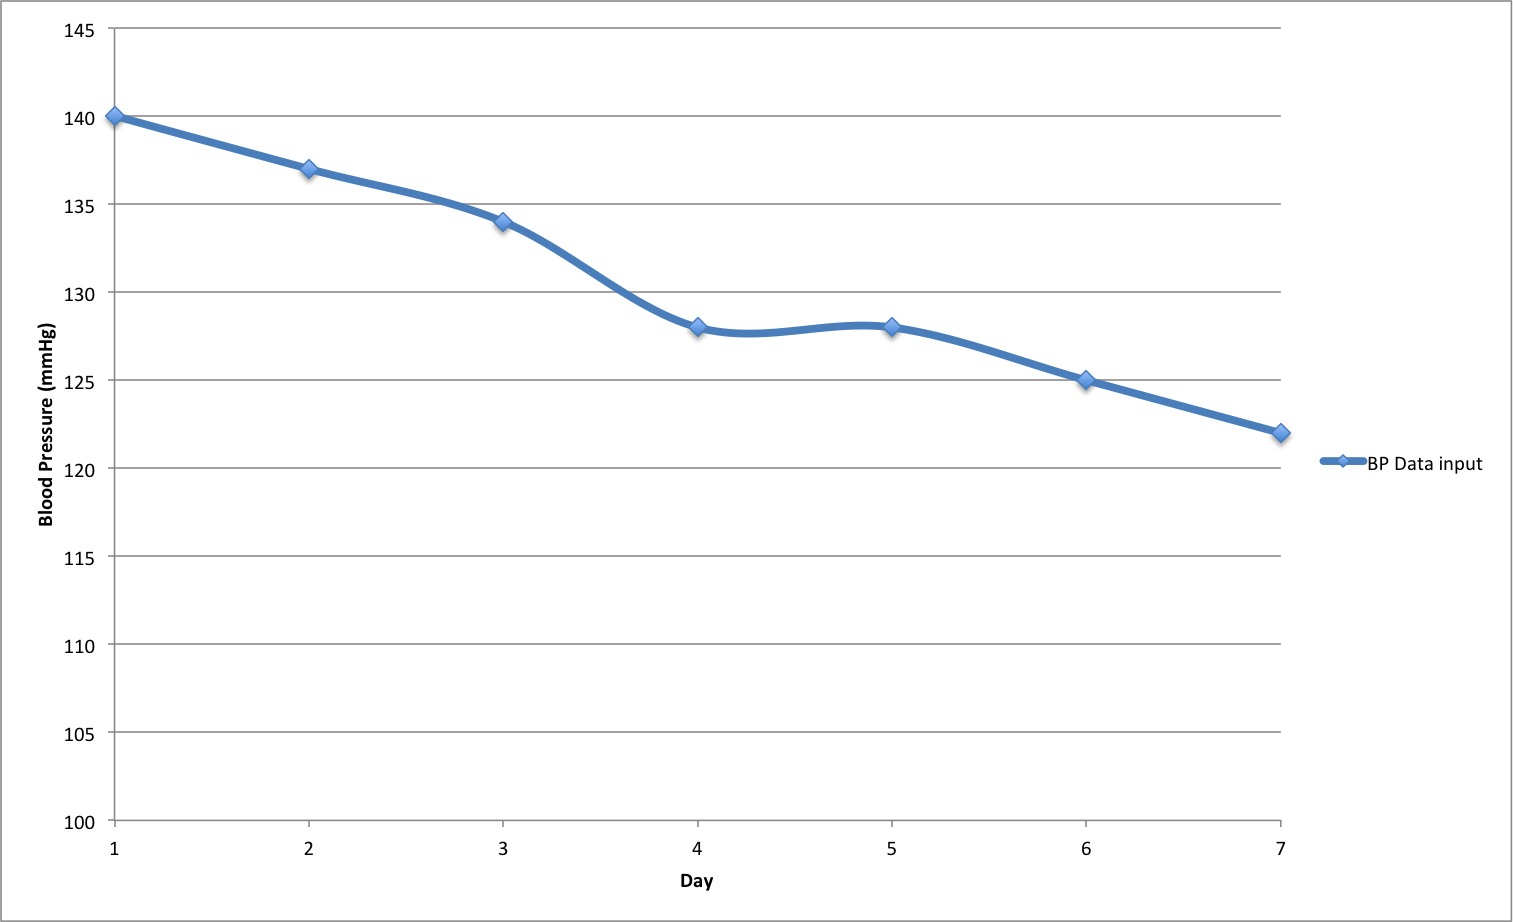
\includegraphics[width=\linewidth]{corrbad.png}}
\caption{Data with an uncertainity metric value of 1}
\endminipage
\end{figure} 

The reason that a large range of limits was chosen is based on two of the limitations that are present in using this method. The prior assumption that data will vary linearly over the 7 day period seems to be contravened, because a perfect set of linearly aligned data (that with a correlation magnitude greater than 0.98) will increase the uncertainty metric. This is why the assumption includes the proviso "with a realistic level of variance" which accounts for the fact that a perfectly correlated data set is statistically significant and suggests that a person may be entering falsified data. The second limitation is that the correlation of a horizontal line is 0, this means that were a patient to enter the same data point each day although there would be minimal variance around the line of best fit the uncertainty metric would not increase as the correlation coefficient would be 0. 

\subsection{Metric Implementation}
To implement the metric within the doctor"s web based application it was necessary to transfer the calculations from Excel file to a script that could be hosted on the application's server. 
\\ \indent There were several ways to do this, initially it was thought that a statistics package such as IBM SPSS 7.0 \cite{SPSS} could be used. The major benefit of such a method is the ease of use; all can be done through the programs graphical user interface (GUI) including linking to the database. The first limitation was that it is not possible to host the program on the server. Data would have to be sent to an external computer and then the results updated into the database. The second limitation is that the cost of purchasing such a package for commercial use is extremely expensive running into tens of thousands of pounds. Hence it is not economically viable for an application such as Cardiac Track that would only use a tiny portion of the program.
\\ \indent 
The solution that was implemented took the form of hard coding the calculations within a PHP script. The main calculation was carried out using a many times nested SQL query and the boundarys checked using "if" statements. 

\subsubsection{Data Input and calculation}
Firstly before any calculations could be performed the patient's last seven data entries, which had not previously been analysed for uncertainty, had to be called from the database. The specific last 7 days were required rather than all data as this was the period of time for which the analysis had been calibrated using the trial patients data.
\\ \indent 
Within the database the patients BP measurements are stored in a database called patientCurrentBP, fig.\ref{DB1}, later the patientFlag column was added to show which data entries have already been analysed.

\begin{wrapfigure}{r}{.60\textwidth}
\centering
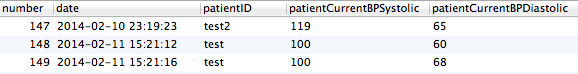
\includegraphics[scale=0.4]{DB1.png}
\caption{Initial patientCurrentBP table \label{DB1}} 
\end{wrapfigure} 

It was initially thought that the best way to call only the 7 previous data variables for a single patient in chronological order was to set up a routine in which an SQL statement would be automatically run on the server periodically. This would input the data from patientCurrentBP to another table, fraudTest where the data could be accessed. It was subsequently found that this was cumbersome and that it was possible to extract the data directly from the currentPatientBP table using an iterative query. The query below must be initialised using a pre query seen on the right that sets the initial value for the iteration.

\begin{figure}[h!] 
\minipage{0.79\textwidth}
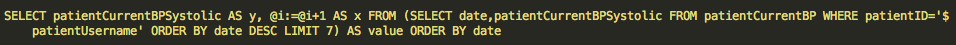
\includegraphics[width=\linewidth]{SQLBPquery.png}
\caption{SQL BP query \label{SQLBPquery}}
\endminipage\hfill
\minipage{0.19\textwidth}
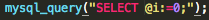
\includegraphics[width=\linewidth]{SQLBPprequery.png}
\caption{SQL BP pre-query}
\endminipage
\end{figure} 

To dissect an SQL statement firstly the innermost query should be considered. The "SELECT" command is retrieving both the date and patientCurrentBPSystolic "FROM" the patientCurrentBP table. 
\begin{wrapfigure}{r}{.25\textwidth}
\centering
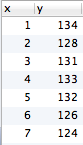
\includegraphics[scale=0.4]{DB2.png}
\caption{Input for SQL calculation \label{DB2}} 
\end{wrapfigure} 
The "WHERE" clause sets the proviso that data only pertaining to the patients own unique username a variable passed at the top of the script should be selected. Finally the "ORDER BY date" puts the data into chronological order and the "DESC LIMT 7" means that only the last seven days are selected as required. The outermost "SELECT" statement now can only select from this set of data, it takes patientCurrentBPsystolic table and the "AS" command calls the data y. The pre-query is then used to cycle through creating the number which corresponds to each day and names it x. This query has thus provided a 2 columned 7rowed table of data, which in y column has the BP measurement, and in the x column the number of the day corresponding to it. This SQL statement can be seen to be imbedded in the bottom of the much larger statement shown in fig.\ref{DB2}. This statement (which has been modified from one developed by Mike Burr \cite{Mike}) calculates both the linear regression and the correlation coefficient. 
\\ \indent
The statement has 4 main sections nested within each other, as with all SQL statements it starts in the middle and works out. The first query section, fig.\ref{SQLBPquery} calls in the raw BP data. Then the next section which is found directly above in the code and finds the values of the components which make up the linear regression and correlation coefficient calculations. 

\begin{wrapfigure}{l}{.50\textwidth}
\centering
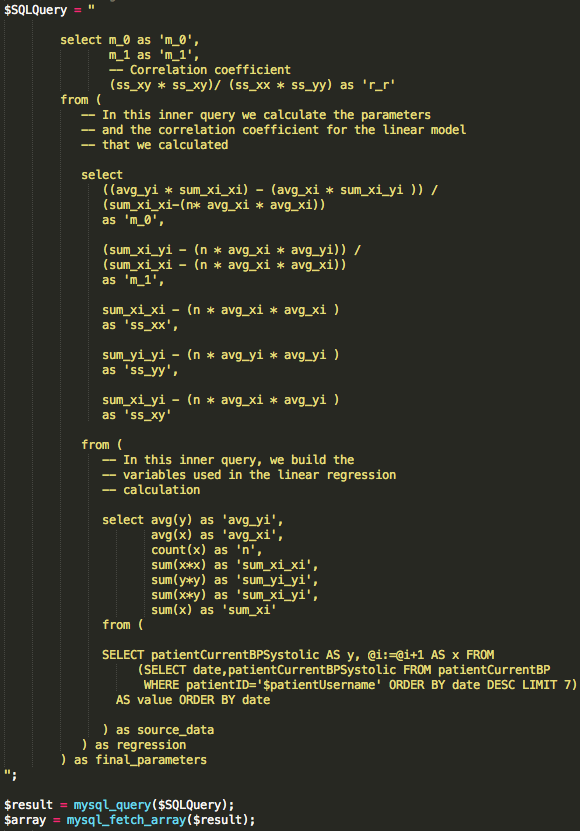
\includegraphics[scale=0.4]{mainSQL.png}
\caption{SQL linear regression and correlation coefficient equation \cite{Mike}} 
\end{wrapfigure} 
The $\overline{x}$ and $\overline{y}$ are simply found using the "avg()" function which finds the mean value of a column. The number of data points is found using the "count()" function. Finally $\Sigma x^2, \Sigma y^2, \Sigma xy, \Sigma x$ can all be calculated by sum(x*x), sum(y*y), sum(x*y) and sum(x) respectively. The sum function adds all values within a column (* denotes multplication of data points). 
\\ \indent
A further step up the page into the next nest segment is where the calculation of both linear regression coefficients, $m_0$ and $m_1$, takes place. This is the implementation of eq.10 and 15, pg.4!!!. The values of the variances$\Sigma x^2 -N\overline{y}\overline{y}, \Sigma y^2 - N\overline{y}\overline{y}, \Sigma xy - N\overline{x}\overline{y}$ are also calculated within and named with the prefixes ss\_xx, ss\_yy and ss\_xy. These are then called in the final nest segment to find the correlation coefficient and so complete the implementation of equation 18, pg 7!!!.
\\ \indent
Finally as shown in the last two lines the query is run in the database using the "mysql\_query" PHP function. The result is formed into an array using the "mysql\_fetch\_array" function. 

\subsubsection{Call the current uncertainty metric value from the data base}

To set the new uncertainty metric the current value of uncertainty attributed to the patient must be called from the database, using the following SQL query: \$patient\_flag\_query = mysql\_query("SELECT fraudFlag FROM patientInfo WHERE patientID='\$patientUsername'"); this gives the variable \$patientFlag. This is the uncertainty metric value for patient currently selected. 

\subsubsection{Calculating limits and test points for patient inputted data}

\begin{wrapfigure}{l}{.25\textwidth}
\centering
\includegraphics[scale=0.6]{corrcheck}
\caption{Correlation coefficient inequalities \label{corrcheck}} 
\end{wrapfigure} 
The simplest limit to test is the correlation coefficient, which is done using two "if" statements, as shown in fig.\ref{corrcheck}. The correlation coefficient variable is called from within the array, it is then placed in an inequality with the boundary value of either +/- 0.98. If the inequality is correct the \$patient\_flag variable is increased by 1 using the PHP ++ incrementation function.
\\ \indent
For the linear regression percentage error limit's test the values of the regression for each day must be calculated. This was initially performed for each of the values individually; top line of fig.\ref{inbound}. Both regression coefficients are called from the array and the $m_1$ value is multiplied by 1 so that the first days value can be found. Once the value has been found in this case labelled \$dayone the +/- 10\% boundaries for this day are calculated using multiplication. 
\begin{wrapfigure}{r}{.42\textwidth}
\centering
\includegraphics[scale=0.6]{linbound}
\caption{Correlation coefficient inequalities \label{inbound}} 
\includegraphics[scale=0.6]{boundtest1}
\caption{Correlation coefficient inequalities} 
\includegraphics[scale=0.6]{dowhile}
\caption{The "do while" loop \label{dowhile}} 
\end{wrapfigure} 

This was coded for all 7 days; the first two are shown in the fig.\ref{inbound}. Following this, a slightly modified version of the SQL statement shown in fig.\ref{SQLBPquery} was used to call the BP data inputted by the patient and format it into an array. This meant that inequalities similar to that used for the correlation coefficient could be used to test whether any points laid outside the linear regression error bounds and modify the \$patient\_flag variable accordingly. The "if" statement inequality on the first line relates the top bound \$dayonetop and the day one patient measured value \$dayin[0] which is selected from the \$dayin array. The bottom bound is checked in the second "if" statement.
\\ \indent 
This section of code was modified firstly into the form of an "if" loop and then once more into a "do while" loop, fig.\ref{dowhile}. The loop, which is initialised with the command "do", contains exactly the same code segments as before however all sections are completed for each day in turn. Once all the values have been calculated and the boundaries checked for one day, an increment is added (\$i++) and the script is run for the next day. The "while (\$i $<$ 7)" in the final line stops the iterations when the increment reaches 6 as the script has been run for all seven days. Although the loop does not improve the codes efficiency, it does mean that it could be more easily modified to accommodate a longer analysis period. It was not possible to investigate the analysis of uncertainty over a longer time period in the scope of this project as the trial data sourced only spanned 7 days. 
\subsubsection{Interaction with currentpatients.php page}
Once the new uncertainty value of the data has been calculated it must be updated in the database. This is done using the following simple update query:
\begin{figure}[h!] 
\includegraphics[width=\linewidth]{finalupdate.png}
\caption{Updating the new uncertainty value to the database}
\end{figure} 

\begin{wrapfigure}{r}{.28\textwidth}
\centering
\includegraphics[scale=0.35]{unbar.png}
\caption{Uncertainty bar} 
\end{wrapfigure} 
This means that it can be called from the database by the currentpatients.php page and be displayed to the doctor. This is done in the form of a bar that fills up, the greater the uncertainty in the data the more of the bar is filled. The bar creation as well as the calling of the linreg.php script is covered within the UI section of the report. A reset button was also implemented within the currentpatents/index.php page so that the doctor can reset the metric to 0 once they have investigated the concern with the patient in question. 

\subsection{Extensions}
There are a couple of ways the current system may be improved upon if more data were present to analyse. Firstly it may be possible to devise whether there are long term trends in patients reactions to hypertension drugs, ie does their effectiveness drop over time. It may also be possible to collaborate with work such as the BioSign monitoring system being developed at OBS Medical Ltd.\cite{OBS} by Prof Lionel Tarassenko. This system tracks the vital signs of a patient in hospital and alerts nurses when the combination of measurements breach calculated bounds. WIth a large amount of data which is hoped to be amassed in the Cardiac Track app it may be possible to implement the uncertainity metrics in a simliar way to BioSign by setting error bounds on a histogram of large previous data sets rather than a linear regression. 

%%%%%%%%%%%%%%%%%%%%%%%%%%%%%%%%%%%%%%%%%%%%%%%%%%%%%%%%%%%%%%%%%%%%%%%%%%%%%%%%%%%%%%%%%%%%%%%%%%%%%%%%%%%

\section{Tallis application}

\subsection{Initial treatment selection - \textit{Emma Saragossi}}
\label{sec:Treatment}

The first course of pharmacological therapy for each patient is determined in the Tallis application. There are 24 possible drug candidates. There are upto 28 arguments for and against each drug. For example the patient's age or ethnicity can determine whether drug can be selected or not.

A \textit{decision} task is populated with the arguments for and against each drug type. There are four types of argument: For (+), Against (-), Confirm (++) and Exclude (--). To demonstrate how they are used, the arguments for and against choosing the ACE Inhibitor \textit{Ramipril} are shown in Table~\ref{table:ramipril}. If a patient has a history of angioedema, hereditary or idiopathic angioedema, renovascular disease, stenosis or is breastfeeding, the drug is excluded from the list of possible candidates. If the patient is of black African or Black Caribbean descent or is over the age of 55, the drug is not excluded from the list but is not recommended. The drug is recommended for patients with heart failure of Myocardial Infarction. If a patient were to have both stenosis and heart failure, for example, while the drug is recommended for those with heart failure, it is contraindicated in patients with stenosis and the drug would not be recommended. The PRO\textit{forma} script for the arguments for and against selecting \textit{Ramipril} is shown in Extract~\ref{code:ramipril}.

\begin{table}[ht]
\begin{center}
\begin{tabular}{| l | l | l | l |}
\hline
\textbf{Comorbidity} & \textbf{Source name} & \textbf{Response} & \textbf{Argument} \\
\hline
History of angioedema & Angio\_expose & Yes & (--) \\
\hline
Renovascular disease & Renovascular & Yes & (--) \\
\hline
Heart failure & Heart\_failure & Yes & (+) \\
\hline
Myocardial Infarction & MI & Yes & (+) \\
\hline
Hereditary or idiopathic angioedema	& Angio\_hered & Yes & (--) \\
\hline
Stenosis & Stenosis & Yes & (--) \\
\hline
Black African or Caribbean & Ethnicity & No & (-) \\
\hline
Over 55 years of age & Age\_group & 55-79 & (-) \\
\hline
Breastfeeding & Breastfeed & Yes & (--) \\
\hline

\end{tabular}
\end{center}
\caption{Arguments for and against selecting ACE Inhibitor \textit{Ramipril}}
\label{table:ramipril}
\end{table}


\begin{code}[ht]
\begin{html}
candidate :: 'ACE__ramipril' ;
          caption :: 'ACE Inhibitor - Ramipril' ;
          argument :: for,Age_group="18-54"            attributes
               argument_name :: 'ACE__ramipril_Arg_01' ;
               caption :: 'Patient is under 55 years of age' ;
          end attributes
          ;
          argument :: for,Ethnicity="No"            attributes
               argument_name :: 'ACE__ramipril_Arg_02' ;
               caption :: 'Patient is not of Black African or Black Caribbean descent' ;
          end attributes
          ;
          argument :: for,Heart_failure="Yes"            attributes
               argument_name :: 'ACE__ramipril_Arg_03' ;
               caption :: 'Patient has heart failure' ;
          end attributes
          ;
          argument :: for,MI="Yes"            attributes
               argument_name :: 'ACE__ramipril_Arg_04' ;
               caption :: 'Patient had a previous MI without heart failure' ;
          end attributes
          ;
          argument :: excluding,angio_expose="Yes"            attributes
               argument_name :: 'ACE__ramipril_Arg_05' ;
               caption :: 'Patient has a history of angioedema associated with previous exposure to an ACE inhibitor' ;
          end attributes
          ;
          argument :: excluding,angio_hered="Yes"            attributes
               argument_name :: 'ACE__ramipril_Arg_06' ;
               caption :: 'Patient has hereditary or idiopathic angioedema' ;
          end attributes
          ;
          argument :: excluding,stenosis="Yes"            attributes
               argument_name :: 'ACE__ramipril_Arg_07' ;
               caption :: 'Patient has bilateral renal artery stenosis' ;
          end attributes
          ;
          argument :: excluding,renovascular="Yes"            attributes
               argument_name :: 'ACE__ramipril_Arg_08' ;
               caption :: 'Patient has known or suspected renovascular disease' ;
          end attributes
          ;
          argument :: excluding,Breastfeed="Yes"            attributes
               argument_name :: 'ACE__ramipril_Arg_09' ;
               caption :: 'Patient is breastfeeding' ;
          end attributes
          ;
          argument :: against,Age_group!="18-54"    attributes
               argument_name :: 'ACE__ramipril_Arg_10' ;
               caption :: 'Patient is older than 55 years of age' ;
          end attributes
          ;
          argument :: against,Ethnicity="Yes"    attributes
               argument_name :: 'ACE__ramipril_Arg_11' ;
               caption :: 'Patient is of Black African or Black Caribbean descent' ;
          end attributes
          ;
\end{html}
\caption{PRO\textit{forma} defining arguments for ACE Inhibitor \textit{Ramipril}}
\label{code:ramipril}
\end{code}

\clearpage

%%%%%%%%%%%%%%%%%%%%%%%%%%%%%%%%%%%%%%%%%%%%%%%%%%%%%%%%%%%%%%%%%%%%%%%%%%%%%%%%%%%%%%%%%%%%%%%%%%%%%%%%%%%
\section{Server Environment - \textit{Henry Fletcher}}
\subsection{Key Project Software}

\subsubsection{PHP: a server-side scripting language}

\textit{PHP: Hypertext Preprocessor} is a general purpose programming language, where its primary use is for creating dynamic website content. PHP is similar in syntax to other languages such as C and Java, and can be used both as a procedural and object-oriented language. It is estimated as of January 2013, PHP was running on nearly 40\% of the world's websites \cite{netcraft:PHP}.
\\ \indent
PHP code is executed entirely on a webserver. The end user effectively receives the output from the PHP processor module, which in the case of a website will usually be formatted HTML. Since PHP is executed on the server, the user does not have access to any of the underlying PHP code, which significantly enhances security. For example, this allows user access control to website pages, which we use extensively in this project.
\\ \indent
Another important use of PHP in creating a website is the ability to create dynamic pages, where the content changes dependent on external inputs. In this project, one of the primary external data inputs was from a MySQL database. Because the data that we were displaying had to change, the use of PHP enables the website content to update from the database every time the page is loaded.

\subsubsection{MySQL: a relational database management system} \label{mysql}

MySQL is widely used, open-source database software, primarily for storing dynamic data that is used on a website. Some of the world's most well known websites use MySQL as their database backend. One of the key parts of this project is the ability to store and share patient data between a patient and a doctor over the Internet and as such the MySQL database that we use is an integral part of the entire project. 
\\ \indent
One of the major reasons for choosing MySQL is its ability to interface with PHP, in the sense that reading and writing data to and from a MySQL database into PHP is relatively easy and very well documented. To interact with the database, a standard language known as SQL (Structured Query Language) is used to send commands to the database server.
\\ \indent
Since this project is handling sensitive patient data and the MySQL database is hosted on a server that is Internet accessible, considerations for data security have to be made. MySQL includes encryption functions as well as user access control to limit who has access to any data stored on it. See section \ref{security} for further security details.

\subsubsection{Apache Web Server}
Apache is the primary HTTP server software that is used in the project. All of the HTML and PHP files are served to the end-user by the Apache software. Apache is one of the most common HTTP servers in existence, serving over half of the world's websites \cite{netcraft:apache}. Apache is fairly modular, in that additional components can be made to work with it, i.e. a PHP module.

\subsubsection{Tallis: clinical decision making software}

Tallis "is a suite of software tools to support authoring, publishing and enacting of clinical knowledge applications over the web" \cite{tallisDescription}. We use Tallis in this project as our medical decision making engine. Tallis Web Enactment (TWE) is the part of the software that runs on the server, and by taking data from both the user and also the MySQL database, it generates intelligent decisions for patient treatment. Tallis Web Enactment runs on top of software known as "Apache Tomcat", which is a Java-based HTTP server.

\subsection{Server Environment Overview} \label{vps}
The test server that was used for the purpose of the project was a Virtual Private Server. This is essentially a 'cloud computer' that runs a full operating system but on shared hardware. Many VPS units will share a single physical server in the data center. The VPS that we used had very limited resources (mainly that it only had 512MB RAM) and as such would not be suitable for running the real 'Cardiac Track' system. The VPS had to run Apache Webserver, Tomcat Webserver, Tallis Web Enactment, and the MySQL database server. In doing so, the test system regularly reached its maximum RAM allocation, which would cause serious performance degradation if real users were using it.

\begin{figure}[ht]
\centering
\includegraphics[scale=0.85]{server-environment-pdf-2}
\caption{Server overview diagram}
\label{server-environment}
\end{figure}


\subsection{Integrating Tallis \& the MySQL database}
One of the important features of our application is the ability for the medical decision making software to access patient data from the database, in order to make tailored decisions for their treatment. The Tallis software can interact with a MySQL database by providing the software with a path to an XML (Extensible Markup Language) file. This XML defines the relationship between a Tallis data variable, via a SQL statement, to an object in the database. One such relationship is called an 'enquiryReader', which reads data from the database and inserts it into Tallis when an enquiry task is called (Code box \ref{xmlenquiryreader}). An enquiry task is a block in Tallis that requires user input, however with database access this data can now be read in from the database automatically. 


%%XML Listing settings!
\lstdefinelanguage{XML}
{
  morestring=[b]",
  morestring=[s]{>}{<},
  morecomment=[s]{<?}{?>},
  stringstyle=\color{black},
  identifierstyle=\color{darkblue},
  keywordstyle=\color{cyan},
  morekeywords={xmlns,version,type,taskName,dataItem,dbName,params}
}

\lstset{
  language        = xml,
  basicstyle      = \small\ttfamily
}  
%%

\renewcommand{\lstlistingname}{Code box}
\begin{lstlisting}[float=ht,numbers=left,frame=lines,caption="Example enquiryReader element",label=xmlenquiryreader,showstringspaces=false]
<enquiryReader taskName="Current_treatment_READ" dataItem="Number_of_drugs">
<preparedSQLStatement dbName="tallis" params="patientID">
SELECT numberDrugs FROM patientDrugs WHERE patientID=(?)
</preparedSQLStatement>
</enquiryReader>
\end{lstlisting}


The 'taskName' attribute defines the name of the Tallis enquiry task that this SQL statement is associated with. The 'dataItem' attribute is the name of the Tallis data variable that will be updated using the output value of the SQL statement. Finally, the 'params' attribute is used to pass any inputs into the SQL statement, in this case the patient's ID number. We use over 500 lines of XML in order to map all of the required data between Tallis and the database.

\subsection{Data storage \& redundancy}
\subsubsection{Database normalisation}
The purpose of a database is to store data in an organised and easily accessible manner.  Additionally, the data should not repeat itself or be redundant in order to be as efficient as possible. To that end, certain rules exist as to how a database such as the one used in this project should be structured. This is known as database normalisation.
\\ \indent
The idea of database normalisation is to correctly organise the data in a database, providing greater flexibility and protection to the data \cite{microsoft:dbnorm}. The rules of normalisation can be applied in rule sets, known as 'normal forms', e.g. "1st Normal Form" and "2nd Normal Form". Higher normal forms by their definition comply with all of the rules given by the lower normal forms, but will include additional requirements. A database's tables must all comply with the nth normal form in order to be considered as an nth order normalised database.
\\
\textbf{1st Normal Form}
\begin{itemize}
\item{"Eliminate repeating groups in individual tables"}
\item{"Create a separate table for each set of related data"}
\item{"Identify each set of data with a primary key" \cite{microsoft:dbnorm}}
\end{itemize}
All of our tables (with one exception) comply with the 1st normal form. The 'patientDrugs' table does not comply, since drugs '1,2,3 and 4' each have a separate column in the database, which violates the first rule of eliminating repeating groups. The 'patientDrugs' table is required to be like this in order to be compatible with the Tallis system.
\\
\textbf{2nd Normal Form}
\begin{itemize}
\item{"Create separate tables for sets of values that apply to multiple records"}
\item{"Relate these tables with a foreign key" \cite{microsoft:dbnorm}}
\end{itemize}
A good example of how we have applied the 2nd normal form is the way that doctors and patients are related. The 'doctorInfo' table contains all of the doctors on our system, each one with their own primary key (identifying number). Subsequently, all of our patient records are linked to a single doctor by including the doctor's ID number in their records. This means if a doctor's address changes, for example, it only needs to be updated in a single record rather than in all of the patient's records. 
\\
\textbf{3rd Normal Form}
\begin{itemize}
\item{"Eliminate fields that do not depend on the key" \cite{microsoft:dbnorm}}
\end{itemize}
The 3rd normal form essentially means that data not directly linked to the first column (e.g. a patient ID number) should be included in a separate table, and then linked to the record if necessary. We believe that the 'doctorInfo' and 'patientInfo' tables comply with the 3rd normal form, since all of the data contained in them relates specifically to that individual.   

\subsubsection{Database scalability}
The Cardiac Track application relies heavily on the MySQL database for it to work. If the application were deployed to a real system, considerations would have to be made about the scalability and redundancy of the database. 
\\
\textbf{Availability:} "The ability to cope with, and .. recover from .. failures" \cite{mysql:chapter15}.
\\
\textbf{Scalability:} "The ability to spread the load of any queries across multiple MySQL servers" \cite{mysql:chapter15}.
\\
There are a number of solutions to ensure that the database system can have high availability and scalability: i) Database replication, ii) Database clustering, iii) Shared-Nothing systems.
\\ \indent
MySQL database \textbf{replication} \cite{mysql:chapter16} is a relatively simple asynchronous master-slave arrangement. The slave servers pull the data off the master server at intervals. This means that additional copies of the data exist on different servers, thus increasing the availability of the data. Additionally, replication can improve read performance to the database, however write performance is often slower, since all writes have to be made to the single master server.
\\ \indent
MySQL \textbf{clustering} \cite{mysql:chapter17} is a more advanced method that involves many interconnected server nodes that operate synchronously with each other. Such systems have no single point of failure, since each node can run on a physically separate machine. Accessing the database can be done by connecting to any one of the nodes, and any changes are propagated to the other nodes instantly. 


\section{Security - \textit{Henry Fletcher}} \label{security}

Since one of the main features of the project is the ability to save and share patient data between patients and clinicians, the project inherently requires the data to be stored somewhere. Since the data is being held on an electronic database, and that data may also contain confidential patient information, the aspect of application security is an important one.
\\ \indent
The primary legislation governing the use and protection of data stored electronically is given by the Data Protection Act \cite{ukDPA}. Additionally, the NHS sets various standards for how patient data should be handled and stored. In order to try and avoid holding personally identifiable information on patients, the 'Cardiac Track App' has been designed to anonymise the data as far as practically possible. To that end, the database does \textit{not} store any of the following: 
\begin{itemize}
  \item Patients real name
  \item Patients data of birth
  \item Patients address or postcode
  \item Medical history not relevant to the application
\end{itemize}
Only a unique identifying name or number is used to link a patient to their record on the application. This name or number could easily be randomly generated. In the event of any data theft or loss from the database, it would be hard for the perpetrator to link the database records to real individuals without first having access to the individuals medical records, which are already stored on the seperate NHS system.

\subsection{NHS Guidelines for data transmission and storage} \label{security:nhsguidelines}
The NHS  has its own recommendations for how data should be handled with regard to encryption. The Government Health \& Social Care Information Centre (HSCIC) publishes guidance on best practice use of encryption when dealing with sensitive data \cite{NHS:hsic:acs}. The guidelines recommend using "greater than or equal to 128 bit" AES encryption for existing systems or, for new deployments, a minimum key size of 256 bits. 
\\ \indent
The guideline also suggests the types of hashing algorithms that are suitable to be used in the NHS (see section \ref{password-hashing} for details on hashing algorithm use in this project). The document recommends the use of SHA-512 or Whirlpool hashing, and explicitly advises against using MD5 or SHA-1, both of which have known security vulnerabilities.


\subsection{SSL Encryption} \label{SSLencryption}
\subsubsection{Overview}
%General overview: Then also the nitty-gritty of implementation including the apache settings? SSL2.0 disabled etc. TLS?
The entire project is based as a web accessible application for both doctors and patients to access. As such, confidential information will be sent and received between the end-users and the server. Normally, Internet traffic is sent 'in the clear', such that if it were to be intercepted by a 3rd party en-route, all of the information being sent between client and server can be obtained. Clearly this is not viable when dealing with potentially confidential material, e.g. patient's blood pressure readings or what drugs they are on for treatment. Fortunately, there is a very common way of being able to send data over the Internet, whilst ensuring its security: Secure Sockets Layer (SSL) and Transport Layer Security (TLS). All manner of major websites that deal with user data such as banks, online shopping, social media and e-mail providers usually employ this system to secure data in transit between their servers and the end-user. SSL/TLS can be thought of as encrypting the data before it is sent over the Internet, and then it is decrypted on arrival at the clients computer. 

\subsubsection{Server configuration}
The NHS HSCIC Guidelines \cite{NHS:hsic:acs} recommend using either SSLv3 or TLSv1.0 or newer. It specifically mandates against using SSLv2, probably since it is officially depreciated and has known security flaws. When setting up the test server SSL settings, it was important to ensure that SSLv2 was disabled to comply with the HSCIC guidelines. 
\\ \indent
The first step of getting SSL to work was to enable the SSL module on the Apache webserver. Then using software called 'OpenSSL', the key and certificate files can be created. Finally, Apache has to be configured to use the key files that are saved on the server. All of these settings are stored in a file, httpd.conf. A snippet of the relevant settings is shown in code box \ref{apachehttpd}.


\begin{lstlisting}[float=ht,numbers=left,frame=lines,caption="Apache httpd.conf",label=apachehttpd,basicstyle=\ttfamily\small,showstringspaces=false]
<VirtualHost *:443>
...
SSLEngine on
SSLOptions +StrictRequire

SSLProtocol -all +TLSv1 +SSLv3
SSLHonorCipherOrder on
SSLCipherSuite HIGH:!SSLv2:!ADH

SSLCertificateFile /etc/apache2/ssl/server2.crt
SSLCertificateKeyFile /etc/apache2/ssl/server2.key
...
</VirtualHost>
\end{lstlisting}


Lines 2 and 4 tell Apache that all requests to port 443 are to be handled using SSL. Port 443 is the port used for HTTP over SSL (HTTPS) \cite{port443}. Lines 6,7 and 8 define the exact type of SSL that is allowed to be used. Initially we use the "-all" flag to disable all of the available protocols, and then we use "+TLSv1 +SSLv3" to enable only these particular protocols. This ensures that SSLv2 remains disabled as required by the NHS guidelines. Note that TLSv1 is the successor to SSLv3 and is marginally more secure. Finally, on lines 10 and 11, we tell Apache where the certificate and key file are stored on the server. These files are required for the encryption process, since they hold the encryption keys.

\subsection{AES encryption}
\subsubsection{Overview}

Although the database which holds all of the application data is secure in the sense that under normal conditions only authorised users and systems will have access to it, there is still a risk that the entire server itself could become compromised and as such the database becomes readable by an un-authorised 3rd party. There are multiple ways to help mitigate against this sort of risk. One of the possible ways is to encrypt all of the data that is stored in the database, so that even if the data is stolen, it would essentially be worthless to someone without the correct key. 
\\ \indent
The NHS guidelines as described in section \ref{security:nhsguidelines} mandate the use of various encryption standards that can be used to encrypt data. In order to encrypt a chunk of textual data, we needed to use a symmetric block cipher. A symmetric cypher uses the same key (password) to encrypt and decrypt the data. One of the primary block ciphers that are used globally is AES (Advanced Encryption Standard). AES with a 256-bit key length is used in the United States for encrypting top-secret information \cite{aes:nsa}, and as such is assumed nearly un-breakable if the key is kept secure. The NHS guideline requirement for using AES-256 therefore ensures that encrypted data remains extremely safe.

\subsubsection{Implementing AES using MySQL}

During the initial stages of the project, the patients iPhone application was built to use AES encryption using the MySQL "AES\_ENCRYPT" command. We chose to use the patient's login password as the encryption key since the plain text password was not stored on the database server, and so if the database was compromised, recovering the encrypted data would be essentially impossible. Code box \ref{mysqlencrypt} shows part of the submission code and SQL statement (shown in red) that was used to encrypt the submitted data before it was saved onto the database.


%%PHP Listing settings!
\lstset{
  language        = php,
  basicstyle      = \small\ttfamily,
  keywordstyle    = \color{dkblue},
  stringstyle     = \color{red},
  identifierstyle = \color{black},
  commentstyle    = \color{dkgreen},
  emph            =[1]{php},
  emphstyle       =[1]\color{black},
  emph            =[2]{if,and,or,else},
  emphstyle       =[2]\color{dkyellow}}
%%

\begin{lstlisting}[float=ht,numbers=left,frame=lines,caption="Example code for submitting patient BP readings with included AES encrypt commands",label=mysqlencrypt,showstringspaces=false]
<?php
...
//Insert the form output into a new row of the patientCurrentBP table
$enterBPquery="INSERT INTO patientCurrentBP VALUES
(now(),AES_ENCRYPT('$id','$input_password'),
AES_ENCRYPT('$sysBP','$input_password'),
AES_ENCRYPT('$diaBP','$input_password'))";
mysql_query($enterBPquery);
?>

\end{lstlisting}


The SQL statement performs a number of actions. Firstly, it is inserting a new row into the "patientCurrentBP" table, which contains all of the submitted patient data. The VALUES command tells the database what data to insert into each column of the new row. In this case, there are 4 columns that exist: The current date and time, the patients ID, their systolic blood pressure, and their diastolic blood pressure. The "now()" command simply inserts the current timestamp into the first column. For the remaining columns, we use MySQL's encryption function to encrypt the patient ID and their blood pressure readings. The function has the format: "AES\_ENCRYPT(\$data, \$key)", and so it is clear that we used the patients password as the encryption key in this case. One thing to note with this example is that both the data and the key is sent un-encrypted to the database server. The encrypt command is only executed by the database and not before, and so the data could potentially travel over the Internet unsecured. However we have mitigated against this sort of loss by using an SSL connection between the client and the server (see section \ref{SSLencryption} for details).
 
\subsubsection{Implementation difficulties and subsequent removal from test system}

Unfortunately because of the nature of this project, encrypting the data would prove to be very difficult, due to the nature of one piece of data needing to accessible to multiple people (i.e. doctor and patient). Additionally, the need for the database access to be compatible with both the application website and the Tallis medical decision engine, meant that any data encryption had to occur using MySQL itself. The default version of AES encryption used by MySQL is 128-bits, rather than the 256-bits required by the NHS. MySQL can however be compiled to use AES-256 if required.
\\ \indent
It became apparent later in the project that the practicalities of getting AES encryption to work across the larger system would significantly complicate the application. The main issue that the project faced was the need for a shared key: if both the doctor and patient need to access the same data, they would both have to use the same encryption key. This would mean the encryption key would have to be stored somewhere on the server so that both users can access the data. However if the  database were compromised, it would be pointless to encrypt the data if the key itself was stored on the compromised database! In a real system, it is likely that a separate secure database or a physical hardware module would be needed to store the encryption key, so that if the primary database were compromised, the key (and hence the data) isn't. Similar approaches are used by Oracle to secure their database products \cite[section 3.1.3]{oracle:keymanagement}.
\\ \indent
As a result, in order to continue to build the application as a prototype demonstration, all of the AES encryption features on the database were removed. It would not be unfeasible to get a full encryption system working given enough time and resources, but the implementation of such a system was deemed to be outside the scope of the project. If the "Cardiac Track" system were ever to be deployed for real world use, a large portion of the code would have to be changed in order to account for an encryption system.

\subsection{Password Hashing} \label{password-hashing}
An important aspect of the project is that both patients and doctors will have access to an online account showing them patient treatment progress. This will require each individual user to have a login name and password, and these details will have to be stored somewhere on the database. A user's password is perhaps one of the most important objects to keep secure when looking at data security. Although users are encouraged not to, many use the same password across all of their Internet identities \cite{ofcom:passwordreport}. This means if a single website becomes compromised, all of those users online accounts could be stolen.
\\ \indent
There is therefore a need to secure the storage of password data when held on a database. The way of doing this is to use a one-way hashing function on the password. Unlike encryption, a hashing function cannot be reversed, and there is no need for complex key management. Modern hash functions are designed to take a variable length input and produce a fixed length output. Additionally, and most importantly for password use, a hash output should be unique for any given input (also known as collision resistance). 

\subsubsection{Example hash functions}

A whole multitude of hashing functions exist for use. Many of the older functions have known vulnerabilities however, which means that choosing the correct function is important when dealing with passwords. An example using the antiquated MD5 algorithm:


\begin{lstlisting}
MD5(Hello World) = b10a8db164e0754105b7a99be72e3fe5
\end{lstlisting}
whereas:
\begin{lstlisting}
MD5(hello world) = 5eb63bbbe01eeed093cb22bb8f5acdc3 
\end{lstlisting}
rightly produces an entirely different output. Other functions, such as SHA-256, use a longer bit length and thus produce longer outputs:
\begin{lstlisting}
SHA256(Hello World) = a591a6d40bf420404a011733cfb7b190d62c65bf0bcda32b...
\end{lstlisting}


\subsubsection{Using hash functions in a login system}
When a doctor first creates a new patient account, the patient has to provide a password. This password is hashed before being saved onto the database. In order to login at a later date, and since the password is stored on the database as an irreversible hash, when the user supplies their password in the login form, that password has to be hashed also in order to be compared with the saved value (see figure \ref{login-flow-diagram}).

\begin{figure}[h]
\centering
\includegraphics[scale=0.85]{passwordhashing-loginform}
\caption{Flow diagram for password checking system}
\label{login-flow-diagram}
\end{figure}

As long as the hashing function remains the same for both password generation and verification, and exactly the correct password is provided, the user will be successfully authenticated. It may therefore seem that the issue of password hashing is solved. Assuming that we use a hashing algorithm that has no vulnerabilities, and  that it cannot be directly reversed regardless of how much computational power you use, then it seems that a user's password will remain hidden even if the database is accessed by a 3rd party. 

\subsubsection{The first problem: Lookup tables} \label{salting}

Unfortunately hash functions are so commonplace, that it is possible to pre-compute every single possible hash of a certain function, and then save all of this data in a lookup table. Additionally, users tend to select their passwords from an extremely small pool of common passwords. Research based on a list of 6 million leaked real passwords comes to the surprising conclusion that the "10,000 most common passwords represent 99.8\% of all user passwords" \cite{xato:top-passwords}.

\begin{figure}[ht]
\centering
\includegraphics[scale=0.4]{passwordsfreq}
\caption{Password use frequency, taken from real 6M data set.}
\cite[image licensed under CC BY-SA 3.0]{xato:top-passwords}
\label{password-use-frequency}
\end{figure}

Therefore, a potential hacker would only need to hash around 10,000 common passwords to create their lookup table. Then it would be a simple task of matching up the stolen hashes to the lookup table. A modern computer could do this within seconds. This vulnerability exploits the fact that users use insecure passwords, as well as the fact that the hash of a text password always returns the same result. 
\\ \indent
The main way to combat lookup table attacks is to use something known as 'salting'. Essentially, a salt is a long random string that is appended onto the end of the users password before it is hashed. Assuming the salt is sufficiently random and long, and that each user has their own salt independent from any other user, it would not be possible to create a lookup table of common passwords for all users. 
\\ \indent 
In order for a system like this to work, the salt actually needs to be saved in plaintext on the database, since in order to check a patient logging in, we need to perform a similar process as previously in figure \ref{login-flow-diagram}. A function call such as:

\begin{lstlisting}
$salt = getUserSaltFromDatabase();
SHA256($inputPassword . $salt) = b10a8db164e0754105b7a99be72e3fe5...
\end{lstlisting}

will create a hash based on the entered input password using the salt for that given user. If that output value then matches the stored value, the password was correct. Note that salting only mitigates against using a pre-generated lookup table. To get around salting, each hash on its own would have to be brute-forced (see section \ref{salting}). With a large database of users, this approach of working on each hash independently would significantly slow hacker attempts to recover the passwords.

\subsubsection{The second problem: Brute-force attacks}
Initially, the majority of hashing algorithms were designed to be fast to compute. This didn't matter, since even just 10 years ago, the computational power to generate every single possible hash combination  was not easily available to a would-be hacker (e.g. creating a hash of every combination of 1,2,3...n character passwords). However it is widely known that computers get exponentially more powerful as time progresses. Moore's Law predicted that the number of transistors on integrated circuits would double in number approximately every two years \cite{moore1965law}. As a result, it is now possible with a modern GPU (Graphics Card) and freely available software to brute-force hashed passwords within minutes.
\\ \indent
Using the MD5 hash algorithm as an example, a modern 2013 graphics card is capable of computing up to 10 billion hashes per second \cite[actual benchmark results]{oclhashcat}. Assume using a password with both upper and lower case letters and the numbers 0-9, gives a character space of 62 different characters. A 7-character password will therefore have up to \(62^7\) different combinations. If this is divided by 10 billion hashes per second, it would take around 1.5 minutes to obtain the password. A GPU in this case is around 100x faster than using a modern CPU.
\\ \indent
Clearly there is a need to mitigate against brute force password attacks, since as compute power continues to increase even longer passwords will be susceptible to being discovered. The primary way of doing this is to use significantly slower hashing algorithms in the first place, as well as employ use of \textit{key stretching}.

%%PHP Listing settings!
\lstset{
  language        = php,
  basicstyle      = \small\ttfamily,
  keywordstyle    = \color{dkblue},
  stringstyle     = \color{red},
  identifierstyle = \color{black},
  commentstyle    = \color{dkgreen},
  emph            =[1]{php},
  emphstyle       =[1]\color{black},
  emph            =[2]{if,and,or,else},
  emphstyle       =[2]\color{dkyellow}}
%%

\begin{lstlisting}[float=ht,numbers=left,frame=lines,caption="Example code for key stretching on SHA-256 algorithm",label=stretching,showstringspaces=false]
<?php
for($i=0;$i<10000;$i++){
    if ($i == 0){
    //Initial hash
    $hash = hash('sha256',$password);
    } 
    else {
    //Subsequent hashes
    $hash = hash('sha256',$hash);
    }
}
?>

\end{lstlisting}


A simple PHP example of key stretching is show  in code box \ref{stretching}. Essentially the result of each hash output is fed back into itself, this is repeated 10,000 times. This means it could take \(10^4\) times longer to brute-force this password hash using the same methods as before, causing a password to be revealed in months or years rather than minutes. The added iterations will slow down the user logging in just slightly, since a hash needs to be computed on every login, but the number of iterations is chosen correctly so that there is minimal user impact (a few tenths of a second is probably acceptable). 

\subsubsection{Hashing implementation in the 'Cardiac Track' application} \label{phpass-section}

Because of the importance of safely storing passwords used by the Cardiac Track application, and the huge number of potential pitfalls involved with password hashing, the project instead uses a "portable public domain password hashing framework" called \textit{phpass} \cite{phpass}. This framework is developed by security experts and includes all of the necessary features to generate a safe cryptographic password hash. In addition to using salting and stretching, the framework also uses a very slow algorithm known as Crypt-Blowfish or \textit{Bcrypt} for short. This algorithm also has a user selectable cost setting, so that over time as compute power increases, the hash can also increase in computational cost \cite{bcrypt}.

\subsection{MySQLi Connector} \label{mysqli}
In section \ref{mysql}, one of the reasons given for using a PHP \& MySQL setup was the ease at which they could be integrated together. PHP can include the MySQL extension functions, which allow database access within PHP. However the way that this extension works is complicated by security issues, with the most dangerous being an SQL injection attack. SQL injection "is a technique where an attacker creates or alters existing SQL commands to expose hidden data, or to override valuable ones, or even to execute dangerous system level commands on the database host" \cite{sqlinjection:phpmanual}. The attack exploits the fact that many database interactions involve a user entering details into a website form before hitting submit. Usually PHP code handles website submission forms by taking the textual input from the forms, turning it into PHP variables, and then  including these variables in a SQL statement, before finally sending and executing the whole SQL statement on the database server. 

\subsubsection{SQL injection example}

%%PHP Listing settings!
\lstset{	 
  language        = php,
  basicstyle      = \small\ttfamily,
  keywordstyle    = \color{dkblue},
  stringstyle     = \color{red},
  identifierstyle = \color{black},
  commentstyle    = \color{dkgreen},
  emph            =[1]{php},
  emphstyle       =[1]\color{black},
  emph            =[2]{if,and,or,else},
  emphstyle       =[2]\color{dkyellow}}
%%

\begin{lstlisting}[float=ht,numbers=left,frame=lines,caption="Example code showing system susceptible to SQL injection",label=sql-injection-1,showstringspaces=false]
<?php
//The username is submitted from the website form and saved as php variable
$username = $_POST['username-form'];
//Include the username variable in the SQL statement:
$query = "SELECT password FROM users WHERE username='$username'";
$result = mysql_query($query);
?>
\end{lstlisting}

Code box \ref{sql-injection-1} shows a very simple system where a user submits their username, and their password is then retrieved from the database. However, this code is very susceptible to an SQL injection attack. Suppose the user entered into the website form the following:

\begin{lstlisting}[showstringspaces=false]
abc'; DROP TABLES users;
\end{lstlisting}

The user has just deleted the 'users' table! If this code is inserted into the full SQL command, it becomes apparent why it works:

\begin{lstlisting}[showstringspaces=false]
$query = "SELECT password FROM users WHERE username='abc'; DROP TABLES users;'";
\end{lstlisting}

By including the single quote mark after the 'abc', the user has escaped outside of the text input area and is now free to issue any SQL command that they choose. The reason this works is that PHP inserts the full value of the variable \$username into the SQL query before it is sent to the database. The MySQL server cannot distinguish between user-entered data and the original SQL statement.

\subsubsection{Mitigating against SQL injection attacks}
Clearly it is important to mitigate against such an attack, especially since our database will hold sensitive patient data. One of the main ways that we protect against unauthorised data access is through user level control written in PHP. However if SQL injection were used, a hacker could easily obtain the data without having a valid login. 
\\ \indent
There are many ways to avoid SQL injection, most of which involve sanitising the data inputs before they are included in the SQL statement. However an easier way is to use the principal of separating data and queries. This is done in PHP using the more advanced MySQLi (MySQL improved) extension, which allows us to separate the data being sent to the database from the SQL query itself. Code box \ref{mysqli-example} demonstrates how this works.

%%PHP Listing settings!
\lstset{
  language        = php,
  basicstyle      = \small\ttfamily,
  keywordstyle    = \color{dkblue},
  stringstyle     = \color{red},
  identifierstyle = \color{black},
  commentstyle    = \color{dkgreen},
  emph            =[1]{php},
  emphstyle       =[1]\color{black},
  emph            =[2]{if,and,or,else},
  emphstyle       =[2]\color{dkyellow}}
%%

\begin{lstlisting}[float=ht,numbers=left,frame=lines,caption="Example code showing MySQLi extension usage",label=mysqli-example,showstringspaces=false]
<?php
//The username is submitted from the website form and saved as php variable
$username = $_POST['username-form'];
//SQL prepared statement
$query = $db->prepare("SELECT password FROM users WHERE username=?");
//Bind parameters
$query->bind_param('s',$username);
$query->execute();
...
?>
\end{lstlisting}

Lines 1-3 are the same as the previous example, however line 5 introduces the concept of a prepared statement. Notice how the question mark (?) on line 5 is used to denote where user input will be required, but is not explicitly included at this point. Line 5 is essentially the 'query' part of our split model system. Not until line 7, where we use the 'bind\_param' function, is the user data added (the 's' means that the username is of type 'String'). This is the 'data' part of the system. Since the PHP variable \$username is not inside the SQL statement, and it is passed to the database server separately and explicitly as data rather than as a query, we have helped to mitigate against SQL injection.
\\ \indent
In this project, not all MySQL/PHP interactions are done using the improved MySQLi connector. However the critical database access involving a user entering data into a form is mostly, if not all, handled using MySQLi, and as such is resistant to an injection attack. For compatibility reasons, some parts of the doctor's portal, which only receive data from the database continue to use the older connector. If this project were transitioned to a real system, it might be preferable to update all of the MySQL access to use the newer connector for security and performance reasons.

\subsection{Other security considerations}
\subsubsection{Application access control} \label{phpsessions}
The project involves patients and doctors being able to 'log-on' to the system in order to use the application. Clearly we need to ensure that a user is correctly authorised before they have access to the system. Additionally, a user should not be able to go directly to a 'secured' page without first having logged in. This access control is achieved by making use of PHP session variables \cite{sessionvars:phpmanual}. Session variables in PHP allow data to be stored and shared between pages. In this case, a session variable is set once a user is successfully logged in. At the top of every PHP page, some code checks to see if this variable exists for the user, and if it does the rest of the page is loaded. If the variable does not exist, then the user is re-directed back to the login page.
\\ \indent
Unlike cookies, session variables are stored on the server. On creating a server-side session variable, the user's browser receives a long unique ID that is randomly generated. This ID is then specific to and only to that user. Each time the user visits a new page, the server requests the ID, and then retrieves any session variables that were stored with that ID. 
\\ \indent
In the case of this application, we save the username as a session variable once the user is successfully logged in. Visits to subsequent pages can use the saved username both to check that the user should have access to that given page, as well as to only display data relevant to that user. If someone bypassed the login process, their username would not be stored as a session variable, and so they would not be able to access the secured pages. Unlike browser cookies, which are saved and can be edited by users on their computers, the user cannot easily edit a server-side session variable.

\subsubsection{Access logging}
Knowing who has accessed and edited data on the system is an important part of the audit trail, especially when handling medical data. Two types of logging occur on the server: The first is explicit logging from PHP code into a database table, and the second occurs automatically by the Apache web server. 
\\ \indent
In practice, an ideal system would log every single user action by both patients and doctors. However for demonstration purposes, the application currently only explicitly logs when a doctor accesses the system. When a doctor logs-in, their user ID, IP address, and the current date and time are recorded in the 'doctorAccessLog' table on the MySQL database.
\\ \indent
The Apache logging occurs by default. It logs in a separate text file every single page request, ordered by timestamp. It includes the IP address of the requesting user, what browser they were using, and what pages they visited. However it does not include in our case who the user was, or what data they entered or accessed. More detailed logging could easily be implemented into the application itself if it were so required.

\subsubsection{Physical hardware security}
The current test server runs as a VPS (explained in section \ref{vps}), and as such resides in a shared data center with no guarantees as to who has access to the physical hardware. Even if the data on the database were encrypted, hardware access by an unauthorised person could allow data to be stolen, since the underlying PHP code would become accessible. 
\\ \indent
If the application were to be run as a real system, additional measures would likely need to be taken to secure the room in which any servers reside. It might even be the case that the application could be hosted by existing systems run by the NHS (though this is unlikely). In any case, strict access control to the servers should be used if they contain sensitive data. This is largely outside of the scope of this demonstration project, however. 

%%%%%%%%%%%%%%%%%%%%%%%%%%%%%%%%%%%%%%%%%%%%%%%%%%%%%%%%%%%%%%%%%%%%%%%%%%%%%%%%%%%%%%%%%%%%%%%%%%%%%%%%%%

\section{Application PHP examples - \textit{Henry Fletcher}}
This section of the project report includes two portions of the actual PHP code used to build parts of the application, namely the login system and the blood pressure submission system. In addition, the entire project codebase can be viewed on github:
\begin{framed}
\url{https://www.github.com/henryfletch/remote-care-application}
\end{framed}
Github was used to store all of the project code. It allows version control, the ability to merge files if edited by multiple people simultaneously, as well as clearly showing line-by-line changes. Since the application was mostly web based, file changes to the github repository immediately updated on the test server. This was achieved using a 'webhook', which essentially notifies the web server of a change, and it then downloads the latest copy of the files \cite{github:webhooks} \cite{github:webhook-2}. 

\subsection{Doctor's Login Form} \label{drloginform}

%%PHP Listing settings!
\lstset{
  language        = php,
  basicstyle      = \small\ttfamily\singlespacing,
  keywordstyle    = \color{dkblue},
  stringstyle     = \color{red},
  identifierstyle = \color{black},
  commentstyle    = \color{dkgreen},
  emph            =[1]{php},
  emphstyle       =[1]\color{black},
  emph            =[2]{if,and,or,else},
  emphstyle       =[2]\color{dkyellow}}
%%

\begin{lstlisting}[numbers=left,frame=lines,label=doctor-login-form,showstringspaces=false]
<?php
// Login Form
// enable sessions
session_start();

// Configure the MySQL connection parameters
$server='remote.villocq.com';
$username='3yp';
$DBpassword='project';
$database='tallis';

// New MySQLi Instance
$db = new mysqli($server,$username,$DBpassword,$database);

//Assign the login form POST output to PHP variables
$id=$_POST['username'];
$input_password=$_POST['password'];

// Get and compare the hashed passwords:
$getHash = $db->prepare("SELECT password FROM doctorInfo WHERE id=?");

// Bind & Execute
$getHash->bind_param('s',$id);
$getHash->execute();
$getHash->bind_result($actual_password_hash);
$getHash->fetch();
$getHash->close();

// Check password matches, using PHPass here
require("PasswordHash.php");
$hasher = new PasswordHash(10,false); // 10 is the cost function setting
$checkPassword = $hasher->CheckPassword($input_password,$actual_password_hash);

// If good password:
if ($checkPassword)  
{
    $_SESSION['userID'] = $id;
    $_SESSION['loginMessage'] = '';
    
    //Add successful login to the Access Log:
    $remoteIP = $_SERVER['REMOTE_ADDR'];
    $doctorLog = $db->prepare("INSERT INTO doctorAccessLog 
    				VALUES('',?,now(),?)");
    $doctorLog->bind_param('ss',$id,$remoteIP);
    $doctorLog->execute();
    $doctorLog->close();
    
header('Location: https://3yp.villocq.com/doctor/index.php'); 
} else {
    $_SESSION['loginMessage'] = 'Incorrect login details. Please try again.';
    header('Location: https://3yp.villocq.com/doctor/loginPage.php'); 
}

$db->close();
?>
\end{lstlisting}

Above is the doctor application "login.php" code. The purpose of the login system is to check that both the user exists and that the entered password is correct. Both the patient and doctor application use a very similar login system. The HTML form, which the user enters their username and password into, is then sent to this PHP code.
\\
\textbf{Line 4} enables PHP session variables, as explained in section \ref{phpsessions}.
\\
\textbf{Lines 7 to 10} contain the details of the MySQL server. The login details are never sent to the client, it remains strictly on the server. Only file access to the server itself can reveal the details. 
\\
\textbf{Line 13} initialises a new MySQLi object. The object handles all of the SQL calls used later in the code.
\\
\textbf{Lines 16 and 17} copy the HTML form variables 'username' and 'password' to internal PHP variables \$id and \$input\_password respectively.
\\
\textbf{Line 20} is the first SQL call to retrieve the user's password hash from the database. It is using the MySQLi prepared statement as described in section \ref{mysqli}. The SQL call returns a password hash only for the exact username match, if there is not an exact match the statement returns 0 records and authentication will fail.
\\
\textbf{Lines 23 to 27} continue with the SQL call. The 'bind\_param' function sends the user ID to the database server, where it is then inserted in place of the question mark (?) in the SQL statement. The 'bind\_result' function allows data to be returned from the SQL call, in this case the \$actual\_password\_hash of that user from the database. 
\\
\textbf{Lines 31 \& 32} make us of the \textit{phpass} (section \ref{phpass-section}) hashing framework. The code creates a new instance of the hashing object, and then passes to it both the password hash that was stored in the database and the entered input password from the login form. The 'CheckPassword' function then encapsulates all that is needed to compare the hash to the provided password. If the stored hash is the same as the hash of the entered password, then the function returns 'true'.
\\
\textbf{Lines 35 to 52} contain all of the actions that occur once a user is successfully authenticated. First some session variables are set which are used later to ensure a user went through the login process (see section \ref{phpsessions}). The 'loginMessage' variable can be used to return error messages in the event of an unsuccessful login. Also included at this stage is some logging: the successful login is recorded into an access log on the database. Finally, the 'header' function redirects the user to the next page of the application, which in this case is the Doctor's portal page.
\\
\textbf{Lines 50 to 52} only happen in the event of the password check being unsuccessful. The 'loginMessage' variable is set to give a generic error message that is displayed to the user, and the header function redirects the user back to the original login page to try again. 

\subsection{Patient's Submission Form}

%%PHP Listing settings!
\lstset{
  language        = php,
  basicstyle      = \small\ttfamily\singlespacing,
  keywordstyle    = \color{dkblue},
  stringstyle     = \color{red},
  identifierstyle = \color{black},
  commentstyle    = \color{dkgreen},
  emph            =[1]{php},
  emphstyle       =[1]\color{black},
  emph            =[2]{if,and,or,else},
  emphstyle       =[2]\color{dkyellow}}
%%

\begin{lstlisting}[numbers=left,frame=lines,label=patient-submit-form,showstringspaces=false]
<?php
session_start();

// Configure the MySQL connection
$server='remote.villocq.com';
$username="3yp";
$DBpassword="project";
$database="tallis";

// New MySQLi Instance
$db = new mysqli($server,$username,$DBpassword,$database);

//Assign the form POST output to PHP variables
$id=$_SESSION['patientAppID'];
$sysBP=$_POST['sysBP'];
$diaBP=$_POST['diaBP'];

//Prepared statement
$submit = $db->prepare("INSERT INTO patientCurrentBP 
			VALUES ('',now(),?,?,?,'0')");

//Bind & Execute to submit to database
$submit->bind_param('sss',$id,$sysBP,$diaBP);
$submit->execute();
// Data has now been submitted!

//// Below code handles the BP target checking ////

//Get the patient's target Systolic BP:
//Prepared statement
$getSystolic = $db->prepare("SELECT targetSystolic 
			    FROM patientInfo WHERE patientID=?");
//Execute and get result
$getSystolic->bind_param('s',$id);
$getSystolic->execute();
$getSystolic->bind_result($targetSystolic);
$getSystolic->fetch();
$getSystolic->close();

//Get the patient's target Diastolic BP:
//Prepared statement
$getDiastolic = $db->prepare("SELECT targetDiastolic 
			     FROM patientInfo WHERE patientID=?");
//Execute and get result
$getDiastolic->bind_param('s',$id);
$getDiastolic->execute();
$getDiastolic->bind_result($targetDiastolic);
$getDiastolic->fetch();
$getDiastolic->close();

//Date checking.
//Get the next review date:
//Prepared statement
$getDate = $db->prepare("SELECT nextReview FROM patientInfo WHERE patientID=?");
//Execute & get
$getDate->bind_param('s',$id);
$getDate->execute();
$getDate->bind_result($reviewDate);
$getDate->fetch();
$getDate->close();

//Now get a difference in days between reviewDate and today (as DaysRemaining)
//Prepared statement
$dateDiff = $db->prepare("SELECT DATEDIFF(?,now()) AS date_difference");
//Execute & get
$dateDiff->bind_param('s',$reviewDate);
$dateDiff->execute();
$dateDiff->bind_result($daysRemaining);
$dateDiff->fetch();
$dateDiff->close();

//Decision Logic for the target BP checking
// First check if review is due:
if ($daysRemaining > 0)
    {
    //Review not due, redirect:
    header("Location: https://3yp.villocq.com/patient/pending.php"); 
    $_SESSION['daysRemaining'] = $daysRemaining;
    }
    
else
    //Review is due:
    {
    // If Systolic is high:
    if ($targetSystolic < $sysBP)
	{  
	echo "Your Systolic BP is too high.";
	echo "<br>";
        $flag = "No"; //i.e bp not controlled
	}
    
    //If Diastolic is high:
    if ($targetDiastolic < $diaBP)
	{  
	echo "Your Diastolic BP is too high.";
	echo "<br>";
        $flag = "No";
	}

    //If BP is lower than target on both:
    if ($targetSystolic >= $sysBP AND $targetDiastolic >= $diaBP)
	{
        $flag = "Yes"; //i.e. bp is controlled
        }
    
    //Now submit the flag to the database.
    //The flag is:BPcontrolled=yes/no
    
    //Prepared statement
    $setFlag = $db->prepare("UPDATE patientInfo SET BPcontrolled=? 
    			     WHERE patientID=?");
    //Execute
    $setFlag->bind_param('ss',$flag,$id);
    $setFlag->execute();
    
    //If flag is set for high BP, refer to Dr. Otherwise goto 'success' page:
    if ($flag == "No") //Reminder: no = BP NOT controlled
        { 
        //Send to alert page
        header("Location: https://3yp.villocq.com/patient/alert.php");
        }
    else
        {
        //Send to continue page
        header("Location: https://3yp.villocq.com/patient/continue.html");
        }
    }
    
$db->close();
?>
\end{lstlisting}

The above code is one of the major parts of the project, which allows the patient to submit their daily blood pressure readings through the application. As well as submitting the BP reading, the application also performs some target-based checks to see if the patient is responding to their treatment. If the target BP is reached successfully, the patient can be told that their treatment is on course and that there is no need to see their doctor.
\\
\textbf{Lines 5 to 24} incorporate all of the code required to submit the patient's blood pressure readings onto the database, in a similar manner to the SQL used for the doctor's login form (section \ref{drloginform}). 
\\
\textbf{Lines 31 to 38 and 42 to 49} retrieve the patient's set target systolic and diastolic blood pressure from the database. The target blood pressures are calculated when the patient first registers with the system.
\\
\textbf{Lines 54 to 60} get the next review date from the database. The review date is set by the Tallis system depending on what drug treatment they are on. Usually the review date is set to be a few weeks after the treatment starts, with the expectation that by this point the patient will have responded to treatment.
\\
\textbf{Lines 64 to 70} use the previous SQL calls to calculate the difference between today and the review date. Effectively the purpose of lines 54 to 70 is to get a number that indicates how many days are left before the patient is considered 'stable' on their treatment plan. The reason this is needed is so that the BP target checking can activate once that value is below 0 days. Before this time, it is likely that their blood pressure might fluctuate too much to infer anything.
\\
\textbf{Lines 74 to 80} occur only if the number of days remaining on the patient's current treatment are greater than zero. If this is the case, no BP checking occurs and the patient is redirected straight to a 'pending' page, where the number of days they have left until their next review is displayed. 
\\
\textbf{Line 81 onwards} occurs if the review is due, i.e. the patient has been on their current line of treatment for long enough to be able to check if they have reached their target blood pressure or not.
\\
\textbf{Lines 84 to 90 and 93 to 98} check to see if the entered blood pressure values exceed the targets. If either the systolic or diastolic is above the target, a flag is set to "No", which means that the patient's blood pressure is "Not Controlled".
\\
\textbf{Lines 100 to 104} do the opposite, and set the flag to "Yes" if the patient's blood pressure is below the targets in both cases.
\\
\textbf{Lines 106 to 114} save the flag value onto the database. This flag is subsequently used on the doctor's application to list the patient as "alerted" or not, as well as by the Tallis decision engine when deciding what treatment to enact.
\\
Finally, \textbf{lines 116 to 126} redirect the patient to one of two pages depending on the value of the flag. If their BP is not controlled (flag set to "No"), they are redirected to an alert page recommending that they visit their doctor. If their BP is controlled (flag set to "Yes") then they are redirected to a sort of 'success' page that instructs them to continue taking their present medication.

%%%%%%%%%%%%%%%%%%%%%%%%%%%%%%%%%%%%%%%%%%%%%%%%%%%%%%%%%%%%%%%%%%%%%%%%%%%%%%%%%%%%%%%%%%%%%%%%%%%%%%%%%%

\section{Economic Viability - \textit{Michael Fedosiuk}}
This section is to show different ways in which the project could be taken forward. Firstly by stating the benefits it has to potential customers, the NHS is focused on however the same arguments apply to a variety of international markets that could also be tapped. Secondly the analysis of the initial cost and future savings predicted from implementing the application. Then a potential rough pricing model and finally what the next steps would be taken.

\subsection{Cost benefits to the customer: Focused on NHS}
There are two potential cost saving benefits the app could present to the NHS. Firstly the reduction of patients who present with diseases caused by hypertension the most common being Stroke and Ischaemic heat disease. All statistics (unless otherwise stated) for this section are taken from two NHS national costing reports. The first being a 2011 report "Hypertension, Costing report, Implementing NICE guidance" \cite{costhome} focused on the relative saving of switching from using clinical blood pressure measurements (CBPM) to either ambulatory (ABPM) or home blood pressure measurements (HMBP) to improve diagnosis. The second published in 2006, titled "Management of hypertension in adults in primary care: partial update, Costing report, Implementing NICE guidance" \cite{costdrug} this report was focused on how patients could be medicated more intensively initially to avoid the possibility of their BP rising above 140 mmHg systolic. The first report was written in 2011 and the second was written in 2006, although this means that some predictions may have changed the general arguments of the report holds true. To bring the reports inline with todays values the costing's in the reports have been increased in line with inflation (22.56\% total compund CPI inflation since 2006 and 3.2\% since 2011). 

\subsubsection{Reduction in Strokes and Ischaemic heart disease} 

\begin{wrapfigure}{r}{0.70\textwidth}
\centering
\includegraphics[scale=0.4]{strokecost.png}
\caption{Costs of Stroke to the NHS and general UK \label{strokecost}} 
\end{wrapfigure}

\textbf{Strokes}
\\
The report states "Approximately 110,000 strokes and a further 20,000 transient ischaemic attacks occur in England each year. Stroke accounts for 11\% of deaths in England." This brings large costs, the national audit office produced the following table, in fig.\ref{strokecost}, in a report "Reducing brain damage: Faster access to better stroke care". The table shows that the estimated cost (\pounds 2.834 Billion in 2006) today of strokes direct to the NHS is approximately \pounds 3.47 Billion; this is a lower bound estimate due to the increase in prevalence of the disease in recent years.
\\ \indent 
The report then stated "It has been calculated that significant reductions in stroke and ischaemic heart disease could be achieved by reducing the blood pressure of everyone with hypertension to a systolic pressure of 140 mmHg. For adults there would be a reduction of 28 to 44\% in stroke and a 20 to 35\% reduction in ischaemic heart disease, depending on age." More over it states that only "40\% of patients achieve their target blood pressure through current prescribing." The app is the direct solution to this problem by alerting a medical professional when a patient breaches a set limit. This would mean that additional medication could be sought to help reduce the patients BP to below 140 mmHg. The report itself tackles this problem by increasing the strength of initial drugs prescribed, these drugs cost more. The app will be able to determine those who are particularly in need of the extra drugs and therefore be more efficient than the apply to all method.
\\ \indent 
Using the blanket all change in medication method the report made the conservative estimate in a 9\% reduction of strokes. Out of the 60\% patients who do not have their hypertension controlled if 16\% required additional drugs, the direct saving to the NHS from stroke prevention will be \pounds 255.1 Million. 
\\
\noindent \textbf{Ischaemic Heart Disease}
\\
It is stated  "a reduction of 5 mmHg in systolic pressure is associated with a reduction in ischaemic heart disease incidence of 11\%" \cite{isch}. This means that even if a reduction to below 140 mmHg is not attainable for some patients, continued treatment to create a 5 mmHg drop would still have markable effects. The NICE report made a conservative estimate of a 4\% reduction in ischaemic heart disease through better treatment. Agreeing with this assumption it followed that with 300000 hospitalisations each year a 4\% reduction is 12000 admittances that were given the average direct to the NHS of \pounds 2582 (in 2006 \pounds 2107). This gives a predicted yearly saving of \pounds 30.98 Million (in 2006 \pounds 25.2 Million). This figure is conservative as it does not incorporated any primary, outpatient or coronary care.
\\
\minipage{\textwidth}
\centering
\textbf{Report predicted a saving of \pounds 343.54 Million (in 2006 \pounds 280.3 Million)}
\endminipage

\subsection{Implementation Costs}

The main cost of implementation would be the purchase of the HBPM. The British Hypertension Society validates 5 monitors 1 costing \pounds 20 and the others \pounds 30. There are 3 potential ways in which these could be rolled out to users of the application.
\begin{enumerate}
\item \textbf{Application is sold to the NHS who provide patients with both the application and home BP monitor}
\\ 
\begin{equation}
Cost=No.Patients * ( AppCost + MonitorCost)
\end{equation}
The number of people treated for hypertension in the UK was 5346902 in 2006 \cite{costdrug}. Taking this figure and the cheapest validated monitor it would cost \pounds 106.98 Million to supply all with a monitor. This is still only around 30\% of the potential \pounds 343.54 Million predicted. It should also be noted that if the NHS were to purchase monitors on such a large scale they would not pay the consumer price \pounds 20. The scale of this purchase would decrease in subsequent years as the monitors validated have a 3 year guarantee. Considering this it would seem reasonable that the NHS could pay for monitors for each patient, as the maximum predicted cost for the largest out lay in the first year would only be around 30\% of the potential saving. 
\item \textbf{Application is sold to the NHS who provide it to patients, however patients must purchase their own home BP monitor}
\begin{equation}
Cost=No.Patients * ( AppCost)
\end{equation}
Although this would be save the NHS a large initial sum, it seems unlikely that this option would be selected. This system would decrease the number of patients who are willing use the diagnosis method. Hence it would also minimise the potential savings to the NHS.
\item \textbf{Application and monitor is sold in tandem to the NHS}
\\
It may be possible to sell the application to a private company in particular one that already make BP monitors. The combined monitor and application could then be sold to health services such as the NHS. An upside is an international company could access foreign markets. The downside to this method is that due to the fact the company will not be the end customer there will be a considerable amount of risk reducing what they would pay for the application.
\end{enumerate}

\subsubsection{Comparables}
\begin{center}
\begin{tabular}{ | p{1.2cm} | p{2.5cm} | p{1cm} | p{10cm} |}
\hline
Icon & Name & Price & Description\\ \hline
\raisebox{-0.7cm}{\includegraphics[width=1cm, height=1cm, scale=0.1]{strides.png}} & Strides & \pounds 2.49 & This is a goal tracking app which just plots changes over time and sets targets. \\ \hline
\raisebox{-1cm}{\includegraphics[width=1cm, height=1cm, scale=0.1]{BPtracker.png}} & Blood Pressure tracker & \pounds 1.49 & Tracks BP, Pulse rate and Mean Arterial Pressure over time. Provides emailable report to doctor. \\ \hline
\raisebox{-0.7cm}{\includegraphics[width=1cm, height=1cm, scale=0.1]{healthcloud.png}} & BP Tracker by Health Cloud & Free & BP and pulse tracking ability to export data in text or CSV formats. \\
\hline
\end{tabular}
\end{center}
All these apps are for the iOS operating system and are therefore purchased from the apple iTunes store \cite{itunes}. They were chosen as comparables as no similar web based app exists. It should be noted that when an app is sold on the iTunes store 30\% of the sale price is given to Apple for hosting costs. 
\\ \indent 
No comparable app has the Cardiac Track App USP the integrated doctor's system. It is the ability to alert the patient and doctor to when a patients hypertension is putting them at risk, this is what adds value for the NHS in the prevention of Strokes and Ischaemic Heart Disease. Given the unique competency it seems reasonable to set a high user price for an app that is completed and fully maintained (i.e. the first pricing model suggestion) at \pounds 3 per user. Cutting 30\% for placement as a native app on iTunes. It must then be realised that in selling directly to the NHS there is only a single major customer, and they will be buying the app users in bulk hence a large discount rate from a user price would have to be agreed upon. If this is set at a 70\% discount it would give a price per unit of 63p. If it were assume that the application would be rolled out to 10\% of patients in the first year revenue of \pounds 2.67 Million would be generated. 

\begin{wrapfigure}{r}{0.40\textwidth}
\centering
\includegraphics[scale=0.4]{costing.png}
\caption{First year predicted income \label{costing}} 
\end{wrapfigure}
The salaries for developers to finish and maintain the app would have to be deducted for 5 full time web developers; on the average salary of \pounds 40000 \cite{salary} would cost \pounds 200000. We require 4 servers to have one dedicated Apache and MySQL and redundancies for both. A suitable server for the predicted number of initial users would be the  would be the PowerEdge R420 costing \pounds4656 for all four \cite{dell}. To use MySQL enterprise edition a licence must be purchased for \pounds3000 \cite{MySQL}. Including a generous contingency this predicts a first year pre tax profit of \pounds3.16 Million if the NHS were to push for implementation if the project at the projected price, fig.\ref{costing}.

%%%%%%%%%%%%%%%%%%%%%%%%%%%%%%%%%%%%%%%%%%%%%%%%%%%%%%%%%%%%%%%%%%%%%%%%%%%%%%%%%%%%%%%%%%%%%%%%%%%%%%%%%%
%ASK HENRY HOW HE DID HIS BIBLIOGRAPHY SO WE CAN GET THEM THE SAME 
%\bibliographystyle{unsrt}
%\bibliography{bibliography}

\begin{thebibliography}{40}
\footnotesize
\begin{singlespace}
\bibitem{webmd1}
Webmd.com. 2014. High Blood Pressure Medication Side Effects. [online] Available at: \url{http://www.webmd.com/hypertension-\\high-blood-pressure/guide/side-effects-high-blood-pressure-medications} [Accessed: 9 Apr 2014].
\bibitem{study}
Larkin, K., Schauss, S., Elnicki, D. and Goodie, J. 2007. Detecting white coat and reverse white coat effects in clinic settings using measures of blood pressure habituation in the clinic and patient self-monitoring of blood pressure. Journal of human hypertension, 21 (7), pp. 516--524.
\bibitem{linregdia}
\url{http://www.marin.edu/~npsomas/Lectures/Ch\_2/Sections\_01to04.html} %not done
\bibitem{Kryzig}
Kreyszig, E., Kreyszig, H. and Norminton, E. J. 2011. Advanced engineering mathematics. [New York]: J. Wiley.
\bibitem{linregdev}
The Mathematical Derivation of Least Squares. 2014. [e-book] Harvard, Psychology. \url{http://isites.harvard.edu/fs/docs/icb.topic515975.files/OLSDerivation.pdf} [Accessed: 9 Apr 2014].
\bibitem{linregex}
Upa.pdx.edu. 2014. [online] Available at: \url{http://www.upa.pdx.edu/IOA/newsom/pa551/scatter2.gif} [Accessed: 9 Apr 2014].
\bibitem{Jquery}
Bibliography: Jquery.Org, J. 2014. jQuery. [online] Available at: \url{http://www.jquery.com} [Accessed: 9 Apr 2014].
\bibitem{SPSS}
Bibliography: Www-01.ibm.com. 2014. IBM - SPSS software - United Kingdom. [online] Available at: \url{http://www-01.ibm.com/software/uk/analytics/spss/} [Accessed: 9 Apr 2014].
\bibitem{Mike}
Burr, M. 2013. Mike's Technology and Finance Blog: SQL Linear Regression. [online] Available at: \url{http://mikemstech.blogspot.co.uk/2013/07/sql-linear-regression.html} [Accessed: 9 Apr 2014].
\bibitem{paint}
Paint v2.0 ( Copyright ©2012 CrazzyWorks) 
\bibitem{chart}
Google-developers.appspot.com. 2014. Visualization: Line Chart - Google Charts - Google Developers. [online] Available at: \url{https://google-developers.appspot.com/chart/interactive/docs/gallery/linechart} [Accessed: 9 Apr 2014].
\bibitem{costhome}
National Institute for Health and Clinical Excellence. 2011. Hypertension Costing report Implementing NICE guidance. National Costing report. [report] NICE. Available at:\url{http://www.nice.org.uk/nicemedia/live/13561/56016/56016.pdf} [Accessed: 9 Apr 2014].
\bibitem{costdrug}
National Institute for Health and Clinical Excellence. 2006.  Management of hypertension in adults in primary care: partial update. Costing report. [report] NICE. Available at:\url{http://www.nice.org.uk/nicemedia/live/13561/56768/56768.pdf} [Accessed: 9 Apr 2014].
\bibitem{isch}
Wald, N. J. and Law, M. R. 2003. A strategy to reduce cardiovascular disease by more than 80\%. Bmj, 326 (7404), p. 1419.
\bibitem{itunes}
Apple.com. 2014. Apple (United Kingdom) - iTunes - Everything you need to be entertained.. [online] Available at: \url{https://www.apple.com/uk/itunes/} [Accessed: 9 Apr 2014].
\bibitem{salary}
Krzysztof Zaucha, W. L. 2014. Web Developer Salaries. [online] Available at: url{http://salary-track.jobs.theguardian.com/salary/Web-Developer-title-salary} [Accessed: 9 Apr 2014].
\bibitem{dell}
Server, P. 2014. New PowerEdge R420. [online] Available at: url{http://www.dell.com/uk/business/p/poweredge-r420/pd} [Accessed: 14 Apr 2014].
\bibitem{MySQL}
Mysql.com. 2014. MySQL :: MySQL Editions. [online] Available at: url{http://www.mysql.com/products/} [Accessed: 14 Apr 2014].
\bibitem{OBS}
Obsmedical.com. 2014. About us - OBS Medical. [online] Available at: url{http://www.obsmedical.com/about-us} [Accessed: 14 Apr 2014].
%%%%%%%%%%%%%%%%%%%%%%%%%%%%%%%%%%%%%%                  %EMMA BIBLOGRAPHY
\bibitem{surveyEngland2009}
Aresu, M., Chaudhury, M., Diment, E., Fuller, E., Gordon-Dseagu, V., Gunning, N., Mindell, J., Nicholson, S., Ogunbadejo, T., Robinson, C., Roth, M., Shelton, N., Tabassum, F., Roderick, P. and Wardle, H. 2010. Volume 1 - health and lifestyles. Health Survey for England 2009. [report] The NHS Information Centre for health and social care, pp. 75-92.
\bibitem{metaSelfMonitoring}
Bray, E. P., Holder, R., Mant, J. and Mcmanus, R. J. 2010. Does self-monitoring reduce blood pressure? Meta-analysis with meta-regression of randomized controlled trials. Annals of medicine, 42 (5), pp. 371--386.
\bibitem{24AmbTreatment}
Conen, D., Tschudi, P. and Martina, B. 2009. Twenty-four hour ambulatory blood pressure for the management of antihypertensive treatment: a randomized controlled trial. Journal of human hypertension, 23 (2), pp. 122--129.
\bibitem{ESH}
Council, E. S., Redon, J., Narkiewicz, K., Nilsson, P. M., Burnier, M., Viigimaa, M., Ambrosioni, E., Coca, A., Olsen, M. H., Schmieder, R. and Others. 2013. 2013 ESH/ESC Guidelines for the management of arterial hypertension. European Heart Journal, 34 pp. 2159--2219.
\bibitem{metaHomeClinic}
Ishikawa, J., Carroll, D. J., Kuruvilla, S., Schwartz, J. E. and Pickering, T. G. 2008. Changes in home versus clinic blood pressure with antihypertensive treatments a meta-analysis. Hypertension, 52 (5), pp. 856--864.
\bibitem{telehealth}
Kvedar, J., Wootton, R. and Dimnick, S. 2006. Home telehealth: connecting care within the community. The Royal Society Medicine Press Ltd London.
\bibitem{telemonitoring}
Moller, D. S., Dideriksen, A., Sorensen, S., Madsen, L. D. and Pedersen, E. B. 2003. Tele-monitoring of home blood pressure in treated hypertensive patients. Blood pressure, 12 (1), pp. 56--62.
\bibitem{CG127}
National Institute for Health and Clinical Excellence (NICE). Hypertension: clinical management of primary hypertension in adults. Clinical Guideline 127. London: NICE; 2011.
\bibitem{comparHomeAmb}
Niiranen, T. J., Kantola, I. M., Vesalainen, R., Johansson, J. and Ruuska, M. J. 2006. A Comparison of Home Measurement and Ambulatory Monitoring of Blood Pressure in the Adjustment of Antihypertensive Treatment*. American journal of hypertension, 19 (5), pp. 468--474.
\bibitem{systTele}
Par\'e, G., Jaana, M. and Sicotte, C. 2007. Systematic review of home telemonitoring for chronic diseases: the evidence base. Journal of the American Medical Informatics Association, 14 (3), pp. 269--277.
\bibitem{SICC}
Parati, G., Stergiou, G. S., Asmar, R., Bilo, G., De Leeuw, P., Imai, Y., Kario, K., Lurbe, E., Manolis, A., Mengden, T. and Others. 2008. European Society of Hypertension guidelines for blood pressure monitoring at home: a summary report of the Second International Consensus Conference on Home Blood Pressure Monitoring. Journal of hypertension, 26 (8), pp. 1505--1526.
\bibitem{CG76}
National Institute for Health and Clinical Excellence. 2009. Medicines adherence - Involving patients in decisions about prescribed medicines and supporting adherence. NICE guideline 76. [report] NICE.
\bibitem{SVG}
Caniuse.com. 2014. Can I use SVG. [online] Available at: http://caniuse.com/svg [Accessed: 16 Apr 2014]
\bibitem{tallisDescription}
COSSAC. 2014. Tallis. [online] Available at: http://www.cossac.org/tallis [Accessed: 21 Apr 2014]
\bibitem{tallisDecision}
COSSAC. 2014. Knowledge Modelling - PRO\textit{forma} tasks. [online] Available at: http://www.cossac.org/technologies/proforma/modelling [Accessed: 21 Apr 2014]
\bibitem{encryption}
NHS Information Governance. 2008. Guidelines on use of encryption to protect person identifiable and sensitive information. [report]
%%%%%%%%%%%%%%%%%%%%%%%%%%%%%%%%%%%%%%                  %END %EMMA %BIBLOGRAPHY
\bibitem{netcraft:PHP}
News.netcraft.com, (2014). PHP just grows \& grows | Netcraft. [online] Available at: \url{http://news.netcraft.com/archives/2013/01/31/php-just-grows-grows.html} [Accessed 22 Apr. 2014].
\bibitem{microsoft:dbnorm}
Support.microsoft.com, (2014). Description of database normalization basics. [online] Available at: \url{http://support.microsoft.com/kb/283878} [Accessed 23 Apr. 2014].
\bibitem{netcraft:apache}
News.netcraft.com, (2014). June 2013 Web Server Survey | Netcraft. [online] Available at: \url{http://news.netcraft.com/archives/2013/06/06/june-2013-web-server-survey-3.html} [Accessed 23 Apr. 2014]
\bibitem{mysql:chapter15}
Dev.mysql.com, (2014). MySQL :: MySQL 5.0 Reference Manual :: 15 High Availability and Scalability. [online] Available at: \url{http://dev.mysql.com/doc/refman/5.0/en/ha-overview.html} [Accessed 22 Apr. 2014].
\bibitem{mysql:chapter16}
Dev.mysql.com, (2014). MySQL :: MySQL 5.0 Reference Manual :: 16 Replication. [online] Available at: \url{http://dev.mysql.com/doc/refman/5.0/en/replication.html} [Accessed 22 Apr. 2014].
\bibitem{mysql:chapter17}
Dev.mysql.com, (2014). MySQL :: MySQL 5.0 Reference Manual :: 17 MySQL Cluster. [online] Available at: \url{http://dev.mysql.com/doc/refman/5.0/en/mysql-cluster.html} [Accessed 22 Apr. 2014].
\bibitem{ukDPA}
Legislation.gov.uk, (2014). Data Protection Act 1998. [online] Available at: \url{http://www.legislation.gov.uk/ukpga/1998/29} [Accessed 23 Apr. 2014].
\bibitem{NHS:hsic:acs}
Government Health \& Social Care Information Centre, (2012). Approved Cryptographic Algorithms Good Practice Guideline. Available at: \url{http://systems.hscic.gov.uk/infogov/security/infrasec/gpg/acs.pdf} [Accessed 23 Apr. 2014].
\bibitem{port443}
Steve Gibson, G. (2014). GRC | Port Authority, for Internet Port 443. [online] Grc.com. Available at: \url{https://www.grc.com/port_443.html} [Accessed 23 Apr. 2014].
\bibitem{aes:nsa}
National Policy on the Use of the Advanced Encryption Standard (AES) to Protect National Security Systems and National Security Information. (2003). [online] Committee on National Security Systems (US). Available at: \url{http://csrc.nist.gov/groups/ST/toolkit/documents/aes/CNSS15FS.pdf} [Accessed 23 Apr. 2014].
\bibitem{oracle:keymanagement}
Docs.oracle.com, (2014). Securing Stored Data Using Transparent Data Encryption. [online] Available at: \url{http://docs.oracle.com/cd/B28359_01/network.111/b28530/asotrans.htm#BABHFIJA} [Accessed 23 Apr. 2014].
\bibitem{ofcom:passwordreport}
Media.ofcom.org.uk, (2014). Ofcom | UK adults taking online password security risks. [online] Available at: \url{http://media.ofcom.org.uk/2013/04/23/uk-adults-taking-online-password-security-risks/} [Accessed 23 Apr. 2014].
\bibitem{xato:top-passwords}
Burnett, M. (2014). 10,000 Top Passwords. [online] Xato - Passwords \& Security. Available at: \url{https://xato.net/passwords/more-top-worst-passwords} [Accessed 23 Apr. 2014].
\bibitem{moore1965law}
Moore, G. and others, (1998). Cramming more components onto integrated circuits. \textit{Proceedings of the IEEE, 86(1), pp.82--85.}
\bibitem{oclhashcat}
Hashcat.net, (2014). oclHashcat - advanced password recovery. [online] Available at: \url{http://hashcat.net/oclhashcat/} [Accessed 23 Apr. 2014].
\bibitem{phpass}
Openwall.com, (2014). Portable PHP password hashing ("password encryption") framework. [online] Available at: \url{http://www.openwall.com/phpass/} [Accessed 23 Apr. 2014].
\bibitem{bcrypt}
Docs.php.net, (2014). PHP: crypt - Manual. [online] Available at: \url{http://docs.php.net/manual/en/function.crypt.php} [Accessed 23 Apr. 2014].
\bibitem{sqlinjection:phpmanual}
Php.net, (2014). PHP: SQL Injection - Manual. [online] Available at: \url{http://www.php.net/manual/en/security.database.sql-injection.php} [Accessed 23 Apr. 2014].
\bibitem{sessionvars:phpmanual}
Php.net, (2014). PHP: Introduction - Manual. [online] Available at: \url{http://www.php.net/manual/en/intro.session.php} [Accessed 23 Apr. 2014].
\bibitem{github:webhooks}
Developer.github.com, (2014). Webhooks | GitHub API. [online] Available at: \url{https://developer.github.com/webhooks/} [Accessed 23 Apr. 2014].
\bibitem{github:webhook-2}
GitHub Gists, (2014). oodavid/README.md. [online] Available at: \url{https://gist.github.com/oodavid/1809044} [Accessed 23 Apr. 2014].
\end{singlespace} 
\end{thebibliography}
%%%%%%%%%%%%%%%%%%%%%%%%%%%%%%%%%%%%%%%%%%%%%%%%%%%%%%%%%%%%%%%%%%%%%%%%%%%%%%%%%%%%%%%%%%%%%%%%%%%%%%%%%%
\end{document}



